\documentclass{article}
%\usepackage[english]{babel}\\%
\usepackage{graphicx}
\usepackage{tabulary}
\graphicspath{ {./images/} }
\usepackage{tabularx}
\usepackage{cancel} 
\usepackage[table,xcdraw]{xcolor}
\usepackage{pdflscape}
\usepackage{lastpage}
\usepackage{multirow}
\usepackage{amsmath}
\usepackage[table]{xcolor}
\usepackage{fixltx2e}
\usepackage[T1]{fontenc}
\usepackage[utf8]{inputenc}
\usepackage{ifthen}
\usepackage{fancyhdr}
\usepackage[document]{ragged2e}
\usepackage[margin=1in,top=1.2in,headheight=57pt,headsep=0.1in]
{geometry}
\usepackage{ifthen}
\usepackage{fancyhdr}
\everymath{\displaystyle}
\usepackage[document]{ragged2e}
\usepackage{fancyhdr}
\everymath{\displaystyle}
%\linespread{2}\\%controls the spacing between lines. Bigger fractions means crowded lines\\%
%\pagestyle{fancy}
%\usepackage[margin=1 in, top=1in, includefoot]{geometry}
%\everymath{\displaystyle}
%\linespread{1.3}\\%controls the spacing between lines. Bigger fractions means crowded lines\\%
%\pagestyle{fancy}
\pagestyle{fancy}
\setlength{\headheight}{56.2pt}

\chead{\ifthenelse{\value{page}=1}{\textbf \textbf Solids Treatment - Question Bank}}
\rhead{\ifthenelse{\value{page}=1}{Shabbir Basrai}{Shabbir Basrai}}
\cfoot{}
\lfoot{Page \thepage\ of \pageref{LastPage}}
\rfoot{Solids Treatment - Question Bank}
\renewcommand{\headrulewidth}{2pt}
\renewcommand{\footrulewidth}{1pt}
%Defining colour with different models.
% \definecolor{mypink1}{rgb}{0.858, 0.188, 0.478}
% \definecolor{mypink2}{RGB}{219, 48, 122}
% \definecolor{mypink3}{cmyk}{0, 0.7808, 0.4429, 0.1412}
% \definecolor{mygray}{gray}{0.6}
% \colorlet{LightRubineRed}{RubineRed!70!}
%colorlet{Mycolor1}{green!10!orange!90!}
%definecolor{Mycolor2}{HTML}{00F9DE}

%New command used in the table with all available colour names
\newcommand{\thiscolor}[1]{\texttt{#1} \hfill \fcolorbox{black}{#1}{\hspace{2mm}}}

%This changes the row separation in the table
\renewcommand{\arraystretch}{1.5}

\cfoot{}
\lfoot{Page \thepage\ of \pageref{LastPage}}
\rfoot{Solids Treatment - Question Bank}
\begin{document}

\textbf{SolidsTreatmentTF}

1. A change in the-pH-of digesting sludge in anaerobic digester is the best early warning indicator of potential digester upset. 

a. True 

b. False 


2. A good maintenance program should be established for all flame arresters to ensure they are all set at the recommended "pop-off' pressures. 

a. True 

b. False 


3. A healthy anaerobic digester should have a carbon dioxide concentration of more than 40\%. 

a. True 

b. False 


4. A high rate anaerobic digester is always heated and mixed. 

a. True
b.False 


5. Anaerobically digested sludge produces gas as a by-product. The gas produced is of little or no value. 

a. True 

b. False 


6. Digester gas containing 60\% methane by volume will likely explode when exposed to a spark or flame. 

a. True 

b. False 


7. Digester gas containing 60\% methane by volume will likely explode when exposed to a spark or flame 

a. True 

b. False 


8. In an anaerobic digester, the [1] is destroyed producing [2]. The digester gas production is typically in the range of [3] cubic feet of digester gas per lb of volatile matter destroyed. 


9. Gas production in an anaerobic digester results from the destruction of fixed solids 

a. True 

b. False 


10. A well operating digester will have a CO2 concentration of greater than 60\% 

a. True 

b. False 


11. Volatile solids removal efficiency of a digester is most commonly monitored utilizing the BOD test

a. True 

b. False 


12. Volatile solids removal efficiency of a digester is most commonly monitored utilizing the BOD test

a. True 

b. False 


13. The range of volatile material in raw sludge may be as high as 60\% - 80\% while digested sludge normally will be below 20\%. 

a. True 

b. False 


14. Foaming in digesters is often due to rapid acid digestion is caused by adding too much raw sludge during too short a time period. 

a. True 

b. False 


15. Aerobic digestion produces methane gas that provides energy for other operations. 

a. True 

b. False 


16. A good maintenance program should be established for all flame arresters to ensure they are all set at the recommended "pop-off" pressures. 

a. True 

b. False 


17. A flame arrester in the gas line between a waste gas burner and an anaerobic digester contains plates which should periodically be inspected and cleaned. 

a. True 

b. False 


18. The methane forming bacteria in an anaerobic digester reproduce more rapidly than the acid forming bacteria. 

a. True 

b. False 


19. The main function of a secondary digester in normal operation is to provide a storage space for seed sludge. 

a. True 

b. False 


20. Supernatant liquor is withdrawn from the lowest possible level in an anaerobic digester. 

a. True 

b. False 


21. The pH of digested sludge in a healthy anaerobic digester will be near 7.0 

a. True 

b. False 


22. Volatile solids reduction is a measure of the effectiveness of an anaerobic digester. 

a. True 

b. False 


23. A properly operated anaerobic, digester functions best within a pH range of 5.4 to 5.8. 

a. True 

b. False 


24. In computing anaerobic digester loadings, it is necessary to take into account the solids lost in the supernatant system. 

a. True 

b. False 


25. In conventional secondary wastewater treatment processes, aerobic decomposition of solids will occur. 

a. True 

b. False 


26. Aerobic digesters are operated under the principle of extended aeration from the activated sludge process. 

a. True 

b. False 


27. After pumping raw sludge to a digester, it is necessary to seal both ends of the line to prevent back siphonage. 

a. True 

b. False 


28. Propeller mixers are located mainly on floating covers of anaerobic digesters rather than on fixed covers. 

a. True 

b. False 


29. A gallon of water weighs 8.34 pounds. A gallon of digested sludge, due to its high volatile content, will weigh much less. 

a. True 

b. False 


30. The range of volatile material in raw sludge may be as high as 60\% - 80\% while digested sludge normally will be below 20\%. 

a. True 

b. False 


31. Foaming in digesters is often due to rapid acid digestion is caused by adding too much raw sludge during too short a time period. 

a. True 

b. False 


32. Aerobic digestion produces methane gas that provides energy for other operations. 

a. True 

b. False 


33. A good maintenance program should be established for all flame arresters to ensure they are all set at the recommended "pop-off" pressures. 

a. True 

b. False 


34. A flame arrester in the gas line between a waste gas burner and an anaerobic digester contains plates which should periodically be inspected and cleaned. 

a. True 

b. False 


35. The methane forming bacteria in an anaerobic digester reproduce more rapidly than the acid forming bacteria. 

a. True 

b. False 


36. The main function of a secondary digester in normal operation is to provide a storage space for seed sludge. 

a. True 

b. False 


37. Supernatant liquor is withdrawn from the lowest possible level in an anaerobic digester. 

a. True 

b. False 


38. The pH of digested sludge in a healthy anaerobic digester will be near 7.0 

a. True 

b. False 


39. Volatile solids reduction is a measure of the effectiveness of an anaerobic digester. 

a. True 

b. False 


40. A properly operated anaerobic, digester functions best within a pH range of 5.4 to 5.8. 

a. True 

b. False 


41. In computing anaerobic digester loadings, it is necessary to take into account the solids lost in the supernatant system. 

a. True 

b. False 


42. In conventional secondary wastewater treatment processes, aerobic decomposition of solids will occur. 

a. True 

b. False 


43. Aerobic digesters are operated under the principle of extended aeration from the activated sludge process. 

a. True 

b. False 


44. After pumping raw sludge to a digester, it is necessary to seal both ends of the line to prevent back siphonage. 

a. True 

b. False 


45. Propeller mixers are located mainly on floating covers of anaerobic digesters rather than on fixed covers. 

a. True 

b. False 


46. A gallon of water weighs 8.34 pounds. A gallon of digested sludge, due to its high volatile content, will weigh much less. 

a. True 

b. False 


47. Gas production in an anaerobic digester results from the destruction of fixed solids in the raw sludge. 

a. True 

b. False 


48. "High rate" and Low rate" when used in referring to an anaerobic digester may refer to the rate of volatile solids loading. 

a. True 

b. False 


49. In computing anaerobic digester loadings, it is necessary to take into account the solids lost in the supernatant system. 

a. True 

b. False 


50. Increased concentrations of volatile acids and decreased alkalinity are the first measurable changes that take place when the process of anaerobic digestion is becoming upset. 

a. True 

b. False 


51. In a gravity thickener the depth of the sludge is kept minimal (<six inches) to avoid solids going over the effluent weir 

a. True 

b. False 


52. In a decanter centrifuge, greater pond depth would produce drier cake 

a. True 

b. False 


53. Sludge thickening is primarily conducted to reduce costs associated with biosolids hauling

a. True 

b. False 


54. Sludge thickening is primarily conducted to reduce costs associated with biosolids hauling 

a. True 

b. False 


55. Gravity thickener is commonly used for sludge dewatering 

a. True 

b. False 


56. Grit and screenings from the preliminary treatment are also considered as biosolids 

a. True 

b. False 


57. In a decanter centrifuge, greater pond depth would produce drier cake 

a. True 

b. False 


58. Sludge thickening is primarily conducted to reduce costs associated with biosolids hauling 

a. True 

b. False 


59. Grit and screenings from the preliminary treatment are also considered as biosolids 

a. True 

b. False 


60. In a gravity thickener the depth of the sludge is kept minimal (<six inches) to avoid solids going over the effluent weir 

a. True 

b. False 


61. Sludge thickening is primarily conducted to reduce costs associated with biosolids hauling

a. True 

b. False 


62. Sludge thickening is primarily conducted to reduce costs associated with biosolids hauling 

a. True 

b. False 


63. Gravity thickener is commonly used for sludge dewatering 

a. True 

b. False 


64. Sludge thickening is primarily conducted to reduce costs associated with biosolids hauling 

a. True 

b. False 

\textbf{BiosolidsTF05192018}

1. Solids treated using a qualified PSRP qualify as Class A biosolids 

a. True 

b. False 


2. Class A and Class B biosolids are two categories of vector reduction requirements of 40 CFR Part 503 

a. True 

b. False 


\textbf{Digestion5}

1. A change in the-pH-of digesting sludge in anaerobic digester is the best early warning indicator of potential digester upset. 

a. True 

b. False 


2. A good maintenance program should be established for all flame arresters to ensure they are all set at the recommended "pop-off' pressures. 

a. True 

b. False 


3. A healthy anaerobic digester should have a carbon dioxide concentration of more than 40\%. 

a. True 

b. False 


4. A high rate anaerobic digester is always heated and mixed. 

a. True
b.False 


5. Anaerobically digested sludge produces gas as a by-product. The gas produced is of little or no value. 

a. True 

b. False 


6. Digester gas containing 60\% methane by volume will likely explode when exposed to a spark or flame. 

a. True 

b. False 


7. In an anaerobic digester, the [1] is destroyed producing [2]. The digester gas production is typically in the range of [3] cubic feet of digester gas per lb of volatile matter destroyed. 


8. Volatile solids removal efficiency of a digester is most commonly monitored utilizing the BOD test

a. True 

b. False 


9. Volatile solids removal efficiency of a digester is most commonly monitored utilizing the BOD test

a. True 

b. False 


10. The range of volatile material in raw sludge may be as high as 60\% - 80\% while digested sludge normally will be below 20\%. 

a. True 

b. False 


11. Foaming in digesters is often due to rapid acid digestion is caused by adding too much raw sludge during too short a time period. 

a. True 

b. False 


12. Aerobic digestion produces methane gas that provides energy for other operations. 

a. True 

b. False 


13. A good maintenance program should be established for all flame arresters to ensure they are all set at the recommended "pop-off" pressures. 

a. True 

b. False 


14. A flame arrester in the gas line between a waste gas burner and an anaerobic digester contains plates which should periodically be inspected and cleaned. 

a. True 

b. False 


15. The methane forming bacteria in an anaerobic digester reproduce more rapidly than the acid forming bacteria. 

a. True 

b. False 


16. The main function of a secondary digester in normal operation is to provide a storage space for seed sludge. 

a. True 

b. False 


17. Supernatant liquor is withdrawn from the lowest possible level in an anaerobic digester. 

a. True 

b. False 


18. The pH of digested sludge in a healthy anaerobic digester will be near 7.0 

a. True 

b. False 


19. Volatile solids reduction is a measure of the effectiveness of an anaerobic digester. 

a. True 

b. False 


20. A properly operated anaerobic, digester functions best within a pH range of 5.4 to 5.8. 

a. True 

b. False 


21. In computing anaerobic digester loadings, it is necessary to take into account the solids lost in the supernatant system. 

a. True 

b. False 


22. In conventional secondary wastewater treatment processes, aerobic decomposition of solids will occur. 

a. True 

b. False 


23. Aerobic digesters are operated under the principle of extended aeration from the activated sludge process. 

a. True 

b. False 


24. After pumping raw sludge to a digester, it is necessary to seal both ends of the line to prevent back siphonage. 

a. True 

b. False 


25. Propeller mixers are located mainly on floating covers of anaerobic digesters rather than on fixed covers. 

a. True 

b. False 


26. A gallon of water weighs 8.34 pounds. A gallon of digested sludge, due to its high volatile content, will weigh much less. 

a. True 

b. False 


27. Gas production in an anaerobic digester results from the destruction of fixed solids in the raw sludge. 

a. True 

b. False 


28. "High rate" and Low rate" when used in referring to an anaerobic digester may refer to the rate of volatile solids loading. 

a. True 

b. False 


29. In computing anaerobic digester loadings, it is necessary to take into account the solids lost in the supernatant system. 

a. True 

b. False 


30. Increased concentrations of volatile acids and decreased alkalinity are the first measurable changes that take place when the process of anaerobic digestion is becoming upset. 

a. True 

b. False 


31. In a two-stage anaerobic digestion system, it is in the secondary tank where most of the volatile solids destruction occurs 

a. True 

b. False 


32. In a two-stage anaerobic digestion system, it is in the secondary tank where most of the volatile solids destruction occurs 

a. True 

b. False 


33. The lower explosive limit for methane is 40\% 

a. True 

b. False 


34. Psychrophilic bacteria would be used in which kind of digester?
(a) Cold digester
(b) Warm digester
(c) Hot digester 

a. True 

b. False 


35. Volatile solids removal efficiency of a digester is most commonly monitored utilizing the BOD test

a. True 

b. False 


36. Sludge digestion is a process by which principally the inorganic matter in sludge is gasified and/or converted to a more stable form by the biological process. 

a. True 

b. False 


37. The determination of the pH on the anaerobic digester is one of the best early warning systems of digester upset. 

a. True 

b. False 


38. The gas produced as part of the anaerobic digestion is of little or no value 

a. True 

b. False 


39. The main function of a secondary digester in normal operation is to provide a storage space for seed sludge. 

a. True 

b. False 


40. The pH of digested sludge in a healthy anaerobic digester will be near 7.0. 

a. True 

b. False 


41. Volatile solids reduction is a measure of the effectiveness of an anaerobic digester. 

a. True 

b. False 


42. Volatile solids removal efficiency of a digester is most commonly monitored utilizing the BOD test 

a. True 

b. False 


43. Volatile solids removal efficiency of a digester is most commonly monitored utilizing the BOD test 

a. True 

b. False 


\textbf{DigestionTF}

1. A change in the-pH-of digesting sludge in anaerobic digester is the best early warning indicator of potential digester upset. 

a. True 

b. False 


2. Digester gas containing 60\% methane by volume will likely explode when exposed to a spark or flame. 

a. True 

b. False 


3. Volatile solids removal efficiency of a digester is most commonly monitored utilizing the BOD test 

a. True 

b. False 


4. Increased concentrations of volatile acids and decreased alkalinity are the first measurable changes that take place when the process of anaerobic digestion is becoming upset. 

a. True 

b. False 


5. Volatile solids removal efficiency of a digester is most commonly monitored utilizing the BOD test 

a. True 

b. False 


6. The gas produced as part of the anaerobic digestion is of little or no value 

a. True 

b. False 


7. Gas production in an anaerobic digester results from the destruction of fixed solids in the raw sludge. 

a. True 

b. False 


8. A healthy anaerobic digester should have a carbon dioxide concentration of more than 40\%. 

a. True 

b. False 


9. "High rate" and Low rate" when used in referring to an anaerobic digester may refer to the rate of volatile solids loading. 

a. True 

b. False 


10. The determination of the pH on the anaerobic digester is one of the best early warning systems of digester upset. 

a. True 

b. False 


11. Sludge digestion is a process by which principally the inorganic matter in sludge is gasified and/or converted to a more stable form by the biological process. 

a. True 

b. False 


12. The pH of digested sludge in a healthy anaerobic digester will be near 7.0. 

a. True 

b. False 


13. Volatile solids reduction is a measure of the effectiveness of an anaerobic digester. 

a. True 

b. False 


14. In computing anaerobic digester loadings, it is necessary to take into account the solids lost in the supernatant system. 

a. True 

b. False 


15. The main function of a secondary digester in normal operation is to provide a storage space for seed sludge. 

a. True 

b. False 


16. A high rate anaerobic digester is always heated and mixed. 

a. True
b.False 


17. A good maintenance program should be established for all flame arresters to ensure they are all set at the recommended "pop-off' pressures. 

a. True 

b. False 


18. Anaerobically digested sludge produces gas as a by-product. The gas produced is of little or no value. 

a. True 

b. False 

\textbf{DigestionTF1a}

1. The range of volatile material in raw sludge may be as high as 60\% - 80\% while digested sludge normally will be below 20\%. 

a. True 

b. False 


2. Foaming in digesters is often due to rapid acid digestion is caused by adding too much raw sludge during too short a time period. 

a. True 

b. False 


3. Aerobic digestion produces methane gas that provides energy for other operations. 

a. True 

b. False 


4. A good maintenance program should be established for all flame arresters to ensure they are all set at the recommended "pop-off" pressures. 

a. True 

b. False 


5. A flame arrester in the gas line between a waste gas burner and an anaerobic digester contains plates which should periodically be inspected and cleaned. 

a. True 

b. False 


6. The methane forming bacteria in an anaerobic digester reproduce more rapidly than the acid forming bacteria. 

a. True 

b. False 


7. The main function of a secondary digester in normal operation is to provide a storage space for seed sludge. 

a. True 

b. False 


8. Supernatant liquor is withdrawn from the lowest possible level in an anaerobic digester. 

a. True 

b. False 


9. The pH of digested sludge in a healthy anaerobic digester will be near 7.0 

a. True 

b. False 


10. Volatile solids reduction is a measure of the effectiveness of an anaerobic digester. 

a. True 

b. False 


11. A properly operated anaerobic, digester functions best within a pH range of 5.4 to 5.8. 

a. True 

b. False 


12. In computing anaerobic digester loadings, it is necessary to take into account the solids lost in the supernatant system. 

a. True 

b. False 


13. In conventional secondary wastewater treatment processes, aerobic decomposition of solids will occur. 

a. True 

b. False 


14. Aerobic digesters are operated under the principle of extended aeration from the activated sludge process. 

a. True 

b. False 


15. After pumping raw sludge to a digester, it is necessary to seal both ends of the line to prevent back siphonage. 

a. True 

b. False 


16. Propeller mixers are located mainly on floating covers of anaerobic digesters rather than on fixed covers. 

a. True 

b. False 


17. A gallon of water weighs 8.34 pounds.  A gallon of digested sludge, due to its high volatile content, will weigh much less. 

a. True 

b. False 


\textbf{Biosolids0a0}

1. Class A and Class B biosolids are two categories of vector reduction requirements of 40 CFR Part 503 

a. True 

b. False 


2. Wastewater sludge stabilized using anaerobic digestion would qualify as Class A biosolid 

a. True 

b. False 


3. Solids treated using a qualified PSRP qualify as Class A biosolids 

a. True 

b. False 


\textbf{SolidsTreatment5a}

1. In a gravity thickener the depth of the sludge is kept minimal (<six inches) to avoid solids going over the effluent weir 

a. True 

b. False 


2. In a decanter centrifuge, greater pond depth would produce drier cake 

a. True 

b. False 


3. Sludge thickening is primarily conducted to reduce costs associated with biosolids hauling

a. True 

b. False 


4. Sludge thickening is primarily conducted to reduce costs associated with biosolids hauling 

a. True 

b. False 


5. Gravity thickener is commonly used for sludge dewatering 

a. True 

b. False 


6. Grit and screenings from the preliminary treatment are also considered as biosolids 

a. True 

b. False 


7. Sludge thickening is primarily conducted to reduce costs associated with biosolids hauling 

a. True 

b. False 


\textbf{Digestion}

1. In an anaerobic digester, the [1] is destroyed producing [2]. The digester gas production is typically in the range of [3] cubic feet of digester gas per lb of volatile matter destroyed. 


2. Calculate the VS loading to the digester in lbs/day if 10,000 cu. ft of sludge containing 4.8\% TS with and an average VS content of 82\% 



3. Calculate the VS loading to the digester in lbs/day if 25,000 gallons of sludge containing 4.5\% TS with and average VS content of 76\% is fed to the digester 



4. Calculate the \% VS reduction in a digester given the volatile solids content of the feed sludge to the digester is 76\% and the volatile solids content of the sludge leaving the digester is 55\% 



5. If an anaerobic digester receives sludge with VS of 76\% and discharges digested sludge with a 56\% VS. Its VS reduction is:

a. 36\% 

b. 48\% 

c. 60\% 

d. 89\% 


6. If an anaerobic digester receives sludge with VS of 80\% and discharges digested sludge with a 60\% VS. Its VS reduction is:

a. 20\% 

b. 25\% 

c. 63\% 

d. 89\% 


7. Calculate the volatile solids reduction in an anaerobic digester given the following information: Raw sludge feed to digester: 73.7\% VS and digested sludge: 57.2\%VS

a. 52.3\% 

b. 64\% 

c. 16.5\% 

d. 42\% 


8. If an anaerobic digester receives sludge with VS of 80\% and discharges digested sludge with a 60\\% VS. Its VS reduction is:

a. 20\% 

b. 25\% 

c. 63\% 

d. 89\% 


9. If an anaerobic digester receives sludge with VS of 80\% and discharges digested sludge with a 60\% VS. Its VS reduction is:

a. 20\% 

b. 25\% 

c. 63\% 

d. 89\% 


10. If an anaerobic digester receives sludge with VS of 80\% and discharges digested sludge with a 60\% VS. Its VS reduction is:

a. 20\% 

b. 25\% 

c. 63\% 

d. 89\% 


11. Volatile solids removal efficiency of a digester is most commonly monitored utilizing the BOD test

a. True 

b. False 


12. If a digester loading is 0.05 lbs VSS/ft3/Day, how large must the digester be if it receives 1,000 lbs. of suspended solids per day with a volatile percentage of 75\%? 

a. 3,750 cu.ft 

b. 10,000 cu.ft 

c. 15,000 cu.ft 

d. 26,666 cu.ft 

e. 37,500 cu.ft 


13. What is the digester efficiency if the volatile solids concentration entering an anaerobic digester is 70\% and the volatile solids concentration leaving the digester is 50\%? 

a. 29\% 

b. 40\% 

c. 57\% 

d. 71\% 


14. You are operating a 1 MGD trickling filter plant with a single stage anaerobic digester You pump about 3,000 gpd of sludge to the fixed cover digester. The supernatant has a BOD of 950 mg/L The BOD loading coming from the supernatant in pounds per day is 

a. 12 

b. 24 

c. 36 

d. 48 


15. How many pounds of solids are pumped to a digester each day, if the digester receives 10,000 gpd of sludge at 5\% density? 

a. 417 lbs/day 

b. 1,497 lbs/day 

c. 2,337 lbs/day 

d. 3,273 lbs/day 

e. 4,170 lbs/day 


16. Primary sludge containing five percent (5\%) solids is pumped to a digester continuously at a rate of 25 gpm. How many pounds of volatile solids are added to the digester each day if the volatile solids content is 73\% of the total solids? 

a. 1,310 lbs/day 

b. 1,800 lbs/day 

c. 9,830 lbs/day 

d. 10,960 lbs/day 

e. 15,010 lbs/day 


17. Thermophilic digestion would take place in: 

a. Imhoff tanks 

b. lagoons 

c. a sanitary sewer system 

d. unheated anaerobic digester 

e. anaerobic digester with temperatures over l00 deg. F 


18. Acid-forming bacteria would be found predominantly in: 

a. aerated grit chambers 

b. aerobic digesters 

c. anaerobic digesters 

d. chlorine contact chambers 

e. a flowing stream with a D.O of 5 mg/1 


19. A pressure relief valve on a fixed roof anaerobic digester is normally set at: 

a. 2 - 4 inches of water column 

b. 6 - 9 inches of water column 

c. 4 inches of mercury column 

d. 8 inches of mercury column 

e. none of the above 


20. Anaerobic digester gas is mainly: 

a. carbon dioxide (CO2) and water ( H2O) 

b. chlorine (Cl2) and ammonia (NH3) 

c. ammonia ( NH3 ) and hydrogen sulfide ( H2S) 

d. carbon dioxide (CO2) and methane (CH4) 

e. carbon dioxide ( CO2 ) and carbon monoxide (CO) 


21. In order for methane formation to occur in an anaerobic digester, the proper environmental conditions must exist. Among these environmental factors are: 

a. pH 

b. alkalinity 

c. volatile acids 

d. detention time 

e. all of the above 


22. When defining BTU (British Thermal Unit), which of the following would apply? 

a. it is the amount of heat required to raise the temperature of one pound of water one degree Fahrenheit 

b. it is the metric system of measure 

c. it is an expression of measurement of water flow over a V-notch weir 

d. it is a thermal coupling used in fail-safe systems on electric motors 

e. none of the above 


23. The primary purpose of a secondary digester is to: 

a. increase gas production 

b. stabilize volatile solids 

c. provide additional storage for detritus 

d. allow for solids separation 

e. none of the above 


24. one of the reasons that air should be excluded from anaerobic digesters is because: 

a. gas storage capacity is reduced 

b. the entrance of air mixed with the gas produced in the digester could create an explosive mixture 

c. air interferes with the action of the aerobic bacteria present 

d. harmful or pathogenic bacteria may be brought in with the air 

e. none of the above 


25. In an on-line treatment facility having three aerobic digesters in series, which of the following statements would be false? 

a. it is not necessary to aerate all three digesters 

b. draw off supernatant from tanks \#2 and \#3 only 

c. a dissolved oxygen level will be easier to maintain in tank \#3 than in tank \#1 

d. sludge pumped to digester \#3 must be thicker than sludge pumped to digester \#2, and \#2 thicker than 1 


26. The volatile acid/alkalinity relationship of an anaerobic digester is an indication of the buffer capacity of the digester contents. When the ratio starts to increase, it indicates: 

a. excellent digester operation 

b. decreases in alkalinity 

c. better methane production 

d. a decrease in volatile acids 

e. an increase in pH 


27. For domestic wastewater, gas production in a well operated anaerobic digester should be in the vicinity of: 

a. 1 cu. ft. of gas per day per pound of volatile matter destroyed 

b. 10 BTU per pound of dry solids at 70\% volatile 

c. one cubic foot of gas per capita per day 

d. 50 BTU per cubic foot 

e. all of the above 


28. What is the purpose of heating and mixing a primary anaerobic digester? 

a. To eliminate all oxygen present 

b. To increase the digestion rate 

c. To keep methane gas in suspension 

d. To prevent settling of grit to the bottom of the digester 


29. Given the following data, what is the most likely cause of the anaerobic digester problem?
DATA: Raw sludge pump on
Digester gas pressure high
Gas pressure relief valve open 

a. Vacuum relief valve stuck open 

b. Too much raw sludge feed 

c. Supernatant line pugged 

d. Digester cover seal broken 


30. The pH in an aerobic digester may decrease due to 

a. The aerobic destruction of alkalinity 

b. Production of CO2 and nitrate ions 

c. Oxidation of H2S to sulfuric acid 

d. An increase in volatile acids 


31. The proper way to start up an anaerobic digester is to fill it 

a. Halfway with seed sludge, then add raw sludge slowly 

b. Up first with raw sludge and wastewater 

c. Up with waste activated sludge 

d. With seed sludge, add lime to pH 10 and mix 


32. How would you determine if a gas mixing system is plugged or otherwise malfunctioning in your anaerobic digester? 

a. By measuring the blower discharge pressure 

b. By measuring the temperature throughout the digester 

c. By observing amount of gas production 

d. By visual observation through the inspection port 


33. Which gas is produced in anaerobic digesters and can be used as a fuel? 

a. Propane 

b. Methane 

c. Ethane 

d. Carbon dioxide 


34. Which one of the following parameter ranges is most appropriate for a healthy anaerobic digester?

a. Volatile solid reduction in the range of 60 to 70\%. 

b. Digester gas production of 7 to 10 ft3 of gas produced per day per pound of volatile solids destroyed. 

c. Alkalinity in the range of 2500 to 3500 mg/L. 

d. Hydrogen sulfide in range of 1\% to 2\% by volume. 

e. Volatile acids in range of 500 to 750 mg/L. 


35. Identify the incorrect statement regarding anaerobic digestion.

a. An anaerobic digester with pH of 7.05, an alkalinity of 2,900 mg/l and a volatile acid concentration of 250 mg/l is probably operating normally. 

b. Sodium bicarbonate may be used in place of lime to neutralize a sour anaerobic digester. 

c. When adding lime to a sour anaerobic digester, it is important to add an excess of this chemical to act as a reservoir of alkalinity. 

d. Ferrous sulfate may be added to an anaerobic digester to reduce hydrogen sulfide concentration where air quality is of concern. 

e. Gas production from anaerobic digester may be expressed as cubic feet of gas produced per pound of volatile matter added per day. 


36. One action that may be taken to improve the health of an anaerobic digester that is going sour would be to:

a. Add small doses of lime daily to maintain the digester pH above 7.0. 

b. Add ferrous sulfate to reduce the concentration of hydrogen sulfide in the digester. 

c. Add seed sludge from a healthy primary digester. 

d. Pump raw sludge to this digester more frequently so that this sludge has a higher pH. 

e. Increase the temperature of the digester to favor a population increase of the methane formers. 


37. Identify the incorrect statement regarding operation of an anaerobic digester.

a. A healthy anaerobic digester would generally have volatile acids in the range of 50 mg/l to 300 mg/l. 

b. The best strategy for pumping raw sludge to an anaerobic digester is to pump it once or twice a day so that the thickest possible raw sludge may be pumped. 

c. An anaerobic digester operating at an alkalinity of 3200 mg/l should be able to tolerate a volatile acid concentration of 250 mg/l. 

d. The change in pH is not a reliable indicator of the changing characteristics of the digesting sludge because the alkalinity in an anaerobic digester acts as a buffer. 

e. The higher the volatile solid content of the primary sludge being fed to the digester, the higher is the expected volatile reduction. 


38. Identify the true statement about anaerobic digesters:

a. Carbon dioxide and methane in digester gas should be 65\% and 35\%, respectively. 

b. Increasing carbon dioxide readings indicate possible organic overload. 

c. Decreasing mixing will always improve recovery of a sour digester. 

d. Increasing the frequency and decreasing the amount of sludge pumping will not improve digester performance. 

e. Reducing the ratio of primary to waste activated sludge will improve gas production. 


39. All of the following are normal operating guidelines for a healthy anaerobic digester except for:

a. A mesophilic digester operating at 93Deg. F to 98Deg. F. 

b. Methane gas in the range of approximately 62\% to 70\%. 

c. Carbon dioxide gas in the range of 30\% to 38\%. 

d. Organic loading to a high rate digester of 0.15 to 0.2 pounds (Lb) volatile Solids per day per ft3 of digester capacity. 

e. Bicarbonate alkalinity in the range of 1500 to 1800. 


40. When adding anhydrous ammonia to a sour primary anaerobic digester, the $\rule{2cm}{0.15mm}$ is an important consideration because if it is too high, digester "poisoning" may result:

a. Concentration of hydrogen sulfide in digester gas. 

b. pH in digesting sludge. 

c. Concentration of free copper ions in digesting sludge 

d. Ferrous and ferric ion concentration in digesting sludge. 

e. Dissolved sulfide concentration. 


41. A true statement regarding the term “biosolids” is:

a. The term is mandated for user by public law 92-500. 

b. The term was developed by US EPA to define all biologically toxic precipitates. 

c. The term is recommended by WEF for “a primarily organic solids product, produced by wastewater treatment processes, that can be beneficially recycled”. 

d. The term is used by the California Water Resources Control Board to include “all insoluble matter derived from living aquatic organisms. 


42. All of the following are normal operating guidelines for a healthy anaerobic digester except for:

a. A mesophilic digester operating at 93Deg. F to 98Deg. F. 

b. Methane gas in the range of approximately 62\% to 70\% 

c. Carbon dioxide gas in the range of 30\% to 38\%. 

d. Organic loading to a high rate digester of 0.15 to 0.2 pounds Lb volatile 

e. Solids per day per ft3 of digester capacity. 

f. Bicarbonate alkalinity in the range of 1500 to 1800. 


43. Ferrous chloride solution is most often added to anaerobic digesters in order to:

a. Reduce corrosion in anaerobic digester walls. 

b. Increase the pH of the digesting sludge. 

c. Add ferrous ion as an essential nutrient. 

d. Precipitate sulfide ions and thereby meet air pollution limits on sulfur emissions. 


44. Anaerobic digester gas is composed mostly of:

a. Carbon dioxide and hydrogen sulfide 

b. Methane and carbon dioxide 

c. Methane and hydrogen sulfide 

d. Methane and carbon monoxide 

e. Methane and ammonia 


45. The range of volatile material in raw sludge may be as high as 60\% - 80\% while digested sludge normally will be below 20\%. 

a. True 

b. False 


46. Foaming in digesters is often due to rapid acid digestion is caused by adding too much raw sludge during too short a time period. 

a. True 

b. False 


47. Aerobic digestion produces methane gas that provides energy for other operations. 

a. True 

b. False 


48. A good maintenance program should be established for all flame arresters to ensure they are all set at the recommended "pop-off" pressures. 

a. True 

b. False 


49. A flame arrester in the gas line between a waste gas burner and an anaerobic digester contains plates which should periodically be inspected and cleaned. 

a. True 

b. False 


50. The methane forming bacteria in an anaerobic digester reproduce more rapidly than the acid forming bacteria. 

a. True 

b. False 


51. The main function of a secondary digester in normal operation is to provide a storage space for seed sludge. 

a. True 

b. False 


52. Supernatant liquor is withdrawn from the lowest possible level in an anaerobic digester. 

a. True 

b. False 


53. The pH of digested sludge in a healthy anaerobic digester will be near 7.0 

a. True 

b. False 


54. Volatile solids reduction is a measure of the effectiveness of an anaerobic digester. 

a. True 

b. False 


55. A properly operated anaerobic, digester functions best within a pH range of 5.4 to 5.8. 

a. True 

b. False 


56. In computing anaerobic digester loadings, it is necessary to take into account the solids lost in the supernatant system. 

a. True 

b. False 


57. In conventional secondary wastewater treatment processes, aerobic decomposition of solids will occur. 

a. True 

b. False 


58. Aerobic digesters are operated under the principle of extended aeration from the activated sludge process. 

a. True 

b. False 


59. After pumping raw sludge to a digester, it is necessary to seal both ends of the line to prevent back siphonage. 

a. True 

b. False 


60. Propeller mixers are located mainly on floating covers of anaerobic digesters rather than on fixed covers. 

a. True 

b. False 


61. A gallon of water weighs 8.34 pounds. A gallon of digested sludge, due to its high volatile content, will weigh much less. 

a. True 

b. False 


62. If an anaerobic digester receives sludge with VS of 76\% and discharges digested sludge with a 56\% VS. Its VS reduction is:

a. 36\% 

b. 48\% 

c. 60\% 

d. 89\% 


63. Calculate the volatile solids reduction in an anaerobic digester given the following information: Raw sludge feed to digester: 73.7 \% VS and digested sludge: 57.2 \%VS

a. 52.3\% 

b. 64\% 

c. 16.5\% 

d. 42\% 


64. If an anaerobic digester receives sludge with VS of 80\% and discharges digested sludge with a 60\% VS. Its VS reduction is:

a. 20\% 

b. 25\% 

c. 63\% 

d. 89\% 


65. If an anaerobic digester receives sludge with VS of 80\% and discharges digested sludge with a 60\% VS. Its VS reduction is:

a. 20\% 

b. 25\% 

c. 63\% 

d. 89\% 


66. If an anaerobic digester receives sludge with VS of 80\% and discharges digested sludge with a 60\% VS. Its VS reduction is:

a. 20\% 

b. 25\% 

c. 63\% 

d. 89\% 


67. If an anaerobic digester receives sludge with VS of 80\% and discharges digested sludge with a 60\% VS. Its VS reduction is:

a. 20\% 

b. 25\% 

c. 63\% 

d. 89\% 


\textbf{DigestionMathMC08122018}

1. If a digester loading is 0.05 lbs VSS/ft3/Day, how large must the digester be if it receives 1,000 lbs. of suspended solids per day with a volatile percentage of 75\%? 

a. 3,750 cu.ft 

b. 10,000 cu.ft 

c. 15,000 cu.ft 

d. 26,666 cu.ft 

e. 37,500 cu.ft 


2. What is the digester efficiency if the volatile solids concentration entering an anaerobic digester is 70\% and the volatile solids concentration leaving the digester is 50\%? 

a. 29\% 

b. 40\% 

c. 57\% 

d. 71\% 


3. You are operating a 1 MGD trickling filter plant with a single stage anaerobic digester You pump about 3,000 gpd of sludge to the fixed cover digester.  The supernatant has a BOD of 950 mg/L The BOD loading coming from the supernatant in pounds per day is 

a. 12 

b. 24 

c. 36 

d. 48 


4. How many pounds of solids are pumped to a digester each day, if the digester receives 10,000 gpd of sludge at 5\% density? 

a. 417 lbs/day 

b. 1,497 lbs/day 

c. 2,337 lbs/day 

d. 3,273 lbs/day 

e. 4,170 lbs/day 


5. Primary sludge containing five percent (5\%) solids is pumped to a digester continuously at a rate of 25 gpm. How many pounds of volatile solids are added to the digester each day if the volatile solids content is 73\% of the total solids? 

a. 1,310 lbs/day 

b. 1,800 lbs/day 

c. 9,830 lbs/day 

d. 10,960 lbs/day 

e. 15,010 lbs/day 


\textbf{SolidsThickeningMathMC08122018}

1. When you spread sludge on agricultural land, the annual application rate of cadmium in the sludge should be less than 2 lbs/acre/year If your sludge contains 30 mg cadmium per kilogram of solids and your plant produces 950,000 lbs per year of dry solids, how many acres do you need? 

a. 3 acres 

b. 14 acres 

c. 19 acres 

d. 27 acres 

\textbf{DigestionMC08122018}

1. Thermophilic digestion would take place in: 

a. Imhoff tanks 

b. lagoons 

c. a sanitary sewer system 

d. unheated anaerobic digester 

e. anaerobic digester with temperatures over l00 Deg. F 


2. Acid-forming bacteria would be found predominantly in: 

a. aerated grit chambers 

b. aerobic digesters 

c. anaerobic digesters 

d. chlorine contact chambers 

e. a flowing stream with a D.O of 5 mg/1 


3. A pressure relief valve on a fixed roof anaerobic digester is normally set at: 

a. 2 - 4 inches of water column 

b. 6 - 9 inches of water column 

c. 4 inches of mercury column 

d. 8 inches of mercury column 

e. none of the above 


4. Anaerobic digester gas is mainly: 

a. carbon dioxide (CO2) and water ( H2O) 

b. chlorine (Cl2) and ammonia (NH3) 

c. ammonia ( NH3 ) and hydrogen sulfide ( H2S) 

d. carbon dioxide (CO2) and methane (CH4) 

e. carbon dioxide ( CO2 ) and carbon monoxide (CO) 


5. In order for methane formation to occur in an anaerobic digester, the proper environmental conditions must exist.  Among these environmental factors are: 

a. pH 

b. alkalinity 

c. volatile acids 

d. detention time 

e. all of the above 


6. When defining BTU (British Thermal Unit), which of the following would apply? 

a. it is the amount of heat required to raise the temperature of one pound of water one degree Fahrenheit 

b. it is the metric system of measure 

c. it is an expression of measurement of water flow over a V-notch weir 

d. it is a thermal coupling used in fail-safe systems on electric motors 

e. none of the above 


7. The primary purpose of a secondary digester is to: 

a. increase gas production 

b. stabilize volatile solids 

c. provide additional storage for detritus 

d. allow for solids separation 

e. none of the above 


8. One of the reasons that air should be excluded from anaerobic digesters is because: 

a. gas storage capacity is reduced 

b. the entrance of air mixed with the gas produced in the digester could create an explosive mixture 

c. air interferes with the action of the aerobic bacteria present 

d. harmful or pathogenic bacteria may be brought in with the air 

e. none of the above 


9. In an on-line treatment facility having three aerobic digesters in series, which of the following statements would be false? 

a. it is not necessary to aerate all three digesters 

b. draw off supernatant from tanks \#2 and \#3 only 

c. a dissolved oxygen level will be easier to maintain in tank \#3 than in tank \#1 

d. sludge pumped to digester \#3 must be thicker than sludge pumped to digester \#2, and \#2 thicker than 1 


10. The volatile acid/alkalinity relationship of an anaerobic digester is an indication of the buffer capacity of the digester contents. When the ratio starts to increase, it indicates: 

a. excellent digester operation 

b. decreases in alkalinity 

c. better methane production 

d. a decrease in volatile acids 

e. an increase in pH 


11. For domestic wastewater, gas production in a well operated anaerobic digester should be in the vicinity of: 

a. 1 cu. ft. of gas per day per pound of volatile matter destroyed 

b. 10 BTU per pound of dry solids at 70\% volatile 

c. one cubic foot of gas per capita per day 

d. 50 BTU per cubic foot 

e. all of the above 


12. What is the purpose of heating and mixing a primary anaerobic digester? 

a. To eliminate all oxygen present 

b. To increase the digestion rate 

c. To keep methane gas in suspension 

d. To prevent settling of grit to the bottom of the digester 


13. Given the following data, what is the most likely cause of the anaerobic digester problem?
DATA:    Raw sludge pump on
                Digester gas pressure high
                Gas pressure relief valve open 

a. Vacuum relief valve stuck open 

b. Too much raw sludge feed 

c. Supernatant line pugged 

d. Digester cover seal broken 


14. The pH in an aerobic digester may decrease due to 

a. The aerobic destruction of alkalinity 

b. Production of CO2 and nitrate ions 

c. Oxidation of H2S to sulfuric acid 

d. An increase in volatile acids 


15. The proper way to start up an anaerobic digester is to fill it 

a. Halfway with seed sludge, then add raw sludge slowly 

b. Up first with raw sludge and wastewater 

c. Up with waste activated sludge 

d. With seed sludge, add lime to pH 10 and mix 


16. How would you determine if a gas mixing system is plugged or otherwise malfunctioning in your anaerobic digester? 

a. By measuring the blower discharge pressure 

b. By measuring the temperature throughout the digester 

c. By observing amount of gas production 

d. By visual observation through the inspection port 


17. Which gas is produced in anaerobic digesters and can be used as a fuel? 

a. Propane 

b. Methane 

c. Ethane 

d. Carbon dioxide 


\textbf{Biosolids}

1. Per Title 40 CFR Part 503, for biosolids to qualify for EQ (Exceptional Quality Standards), it must meet 

a. Pollution concentration limits 

b. Class A Pathogen Standard 

c. Vector Reduction Standard 

d. All of the above 


\textbf{Digestion Question Bank}

1. Calculate the VS loading to the digester in lbs/day if 10,000 cu. ft of sludge containing 4.8\% TS with and an average VS content of 82\%



2. Calculate the VS loading to the digester in lbs/day if 25,000 gallons of sludge containing 4.5\% TS with and average VS content of 76\% is fed to the digester



3. Calculate the \% VS reduction in a digester given the volatile solids content of the feed sludge to the digester is 76\% and the volatile solids content of the sludge leaving the digester is 55\%



4. If an anaerobic digester receives sludge with VS of 76\% and discharges digested sludge with a 56\% VS. Its VS reduction is:

a. 36\% 

b. 48\% 

c. 60\% 

d. 89\% 


5. If an anaerobic digester receives sludge with VS of 80\% and discharges digested sludge with a 60\% VS. Its VS reduction is:

a. 20\% 

b. 25\% 

c. 63\% 

d. 89\% 


6. Calculate the volatile solids reduction in an anaerobic digester given the following information: Raw sludge feed to digester: 73.7 \% VS and digested sludge: 57.2 \%VS

a. 52.3\% 

b. 64 

c. 16.5\% 

d. 42\% 


7. If an anaerobic digester receives sludge with VS of 80\% and discharges digested sludge with a 60\% VS. Its VS reduction is:

a. 20\% 

b. 25\% 

c. 63\% 

d. 89\% 


8. If an anaerobic digester receives sludge with VS of 80\% and discharges digested sludge with a 60\% VS. Its VS reduction is:

a. 20\% 

b. 25\% 

c. 63\% 

d. 89\% 


9. If an anaerobic digester receives sludge with VS of 80\% and discharges digested sludge with a 60\% VS. Its VS reduction is:

a. 20\% 

b. 25\% 

c. 63\% 

d. 89\% 


10. Volatile solids removal efficiency of a digester is most commonly monitored utilizing the BOD test

a. True 

b. False 


11. In an anaerobic digester, the [1] is destroyed producing [2]. The digester gas production is typically in the range of [3] cubic feet of digester gas per lb of volatile matter destroyed. 


12. In an anaerobic digester, the [1] is destroyed producing [2]. The digester gas production is typically in the range of [3] cubic feet of digester gas per lb of volatile matter destroyed. 


13. Calculate the VS loading to the digester in lbs/day if 10,000 cu. ft of sludge containing 4.8\% TS with and an average VS content of 82\% 



14. Calculate the VS loading to the digester in lbs/day if 25,000 gallons of sludge containing 4.5\% TS with and average VS content of 76\% is fed to the digester 



15. Calculate the \% VS reduction in a digester given the volatile solids content of the feed sludge to the digester is 76\% and the volatile solids content of the sludge leaving the digester is 55\% 



16. Calculate the organic loading rate to two 320,000 gallon anaerobic digesters given:
Primary sludge feed rate of 25,000 gallons with 6.2\% TS containing 73\% solids and SG of 1.03.
Secondary sludge feed rate of 30,500 gallons with 3.8\% TS containing 77\% solids (7 points)
(Answer: 0.2lbs VS/day-ft3 ) 



17. If an anaerobic digester receives sludge with VS of 76\% and discharges digested sludge with a 56\% VS. Its VS reduction is: 

a. 36\% 

b. 48\% 

c. 60\% 

d. 89\% 


18. Calculate the volatile solids reduction in an anaerobic digester given the following information: Raw sludge feed to digester: 73.7 \% VS and digested sludge: 57.2 \%VS 

a. 52.3\% 

b. 64 

c. 16.5\% 

d. 42\% 


19. If an anaerobic digester receives sludge with VS of 80\% and discharges digested sludge with a 60\% VS. Its VS reduction is: 

a. 20\% 

b. 25\% 

c. 63\% 

d. 89\% 


20. Calculate the VS loading to the digester in lbs/day if 10,000 cu. ft of sludge containing 4.8\% TS with and an average VS content of 82\% 

a. 42,756 lbs/day 

b. 24,554 lbs/day 

c. 30,987 lbs/day 

d. 3,256 lbs/day 


21. Calculate the VS loading to the digester in lbs/day if 25,000 gallons of sludge containing 4.5\% TS with and average VS content of 76\% is fed to the digester 

a. 7,131 lbs/day 

b. 17,432 lbs/day 

c. 19,256 lbs/day 

d. 26,244 lbs/day 


22. Calculate the \% VS reduction in a digester given the volatile solids content of the feed sludge to the digester is 76\% and the volatile solids content of the sludge leaving the digester is 55\% 

a. 56\% 

b. 38\% 

c. 42\% 

d. 61.4\% 


23. What is the digester efficiency if the volatile solids concentration entering an anaerobic digester is 70\% and the volatile solids concentration leaving the digester is 50\%? 

a. 29\% 

b. 40\% 

c. 57\% 

d. 71\% 


24. You are operating a 1 MGD trickling filter plant with a single stage anaerobic digester You pump about 3,000 gpd of sludge to the fixed cover digester. The supernatant has a BOD of 950 mg/L The BOD loading coming from the supernatant in pounds per day is 

a. 12 

b. 24 

c. 36 

d. 48 


25. How many pounds of solids are pumped to a digester each day, if the digester receives 10,000 gpd of sludge at 5\% density? 

a. 417 lbs/day 

b. 1,497 lbs/day 

c. 2,337 lbs/day 

d. 3,273 lbs/day 

e. 4,170 lbs/day 


26. Primary sludge containing five percent (5\%) solids is pumped to a digester continuously at a rate of 25 gpm. How many pounds of volatile solids are added to the digester each day if the volatile solids content is 73\% of the total solids? 

a. 1,310 lbs/day 

b. 1,800 lbs/day 

c. 9,830 lbs/day 

d. 10,960 lbs/day 

e. 15,010 lbs/day 


27. Calculate the volatile solids reduction in an anaerobic digester given the following information: Raw sludge feed to digester: 73.7 \% VS and digested sludge: 57.2 \%VS 

a. 52.3\% 

b. 64 

c. 16.5\% 

d. 42\% 


28. If an anaerobic digester receives sludge with VS of 76\% and discharges digested sludge with a 56\% VS. Its VS reduction is: 

a. 36\% 

b. 48\% 

c. 60\% 

d. 89\% 


29. Calculate the volatile solids reduction in an anaerobic digester given the following information: Raw sludge feed to digester: 73.7 \% VS and digested sludge: 57.2 \%VS 

a. 52.3\% 

b. 64 

c. 16.5\% 

d. 42\% 


30. If an anaerobic digester receives sludge with VS of 80\% and discharges digested sludge with a 60\% VS. Its VS reduction is: 

a. 20\% 

b. 25\% 

c. 63\% 

d. 89\% 


31. If a digester loading is 0.05 lbs VSS/ft3/Day, how large must the digester be if it receives 1,000 lbs. of suspended solids per day with a volatile percentage of 75\%? 

a. 3,750 cu.ft 

b. 10,000 cu.ft 

c. 15,000 cu.ft 

d. 26,666 cu.ft 

e. 37,500 cu.ft 


32. What is the digester efficiency if the volatile solids concentration entering an anaerobic digester is 70\% and the volatile solids concentration leaving the digester is 50\%? 

a. 29\% 

b. 40\% 

c. 57\% 

d. 71\% 


33. You are operating a 1 MGD trickling filter plant with a single stage anaerobic digester You pump about 3,000 gpd of sludge to the fixed cover digester. The supernatant has a BOD of 950 mg/L The BOD loading coming from the supernatant in pounds per day is 

a. 12 

b. 24 

c. 36 

d. 48 


34. How many pounds of solids are pumped to a digester each day, if the digester receives 10,000 gpd of sludge at 5\% density? 

a. 417 lbs/day 

b. 1,497 lbs/day 

c. 2,337 lbs/day 

d. 3,273 lbs/day 

e. 4,170 lbs/day 


35. Primary sludge containing five percent (5\%) solids is pumped to a digester continuously at a rate of 25 gpm. How many pounds of volatile solids are added to the digester each day if the volatile solids content is 73\% of the total solids? 

a. 1,310 lbs/day 

b. 1,800 lbs/day 

c. 9,830 lbs/day 

d. 10,960 lbs/day 

e. 15,010 lbs/day 


36. If a digester loading is 0.05 lbs VSS/ft3/Day, how large must the digester be if it receives 1,000 lbs. of suspended solids per day with a volatile percentage of 75\%? 

a. 3,750 cu.ft 

b. 10,000 cu.ft 

c. 15,000 cu.ft 

d. 26,666 cu.ft 

e. 37,500 cu.ft 


37. If an anaerobic digester receives sludge with VS of 76\% and discharges digested sludge with a 56\% VS. Its VS reduction is: 

a. 36\% 

b. 48\% 

c. 60\% 

d. 89\% 


38. Calculate the volatile solids reduction in an anaerobic digester given the following information: Raw sludge feed to digester: 73.7 \% VS and digested sludge: 57.2 \%VS 

a. 52.3\% 

b. 64 

c. 16.5\% 

d. 42\% 


39. If an anaerobic digester receives sludge with VS of 80\% and discharges digested sludge with a 60\% VS. Its VS reduction is: 

a. 20\% 

b. 25\% 

c. 63\% 

d. 89\% 


40. Anaerobic digester gas is composed mostly of: 

a. Carbon dioxide and hydrogen sulfide 

b. Methane and carbon dioxide 

c. Methane and hydrogen sulfide 

d. Methane and carbon monoxide 

e. Methane and ammonia 


41. A true statement regarding the term “biosolids” is: 

a. The term is mandated for user by public law 92-500. 

b. The term was developed by US EPA to define all biologically toxic precipitates. 

c. The term is recommended by WEF for “a primarily organic solids product, produced by wastewater treatment processes, that can be beneficially recycled”. 

d. The term is used by the California Water Resources Control Board to include “all insoluble matter derived from living aquatic organisms. 


42. A true statement regarding the term “biosolids” is: 

a. The term is mandated for user by public law 92-500. 

b. The term was developed by US EPA to define all biologically toxic precipitates. 

c. The term is recommended by WEF for “a primarily organic solids product, produced by wastewater treatment processes, that can be beneficially recycled”. 

d. The term is used by the California Water Resources Control Board to include “all insoluble matter derived from living aquatic organisms. 


43. Which one of the following parameter ranges is most appropriate for a healthy anaerobic digester? 

a. Volatile solid reduction in the range of 60 to 70\%. 

b. Digester gas production of 7 to 10 ft3 of gas produced per day per pound of volatile solids destroyed. 

c. Alkalinity in the range of 2500 to 3500 mg/L. 

d. Hydrogen sulfide in range of 1\% to 2\% by volume. 

e. Volatile acids in range of 500 to 750 mg/L. 


44. Identify the incorrect statement regarding anaerobic digestion. 

a. An anaerobic digester with pH of 7.05, an alkalinity of 2,900 mg/l and a volatile acid concentration of 250 mg/l is probably operating normally. 

b. Sodium bicarbonate may be used in place of lime to neutralize a sour anaerobic digester. 

c. When adding lime to a sour anaerobic digester, it is important to add an excess of this chemical to act as a reservoir of alkalinity. 

d. Ferrous sulfate may be added to an anaerobic digester to reduce hydrogen sulfide concentration where air quality is of concern. 

e. Gas production from anaerobic digester may be expressed as cubic feet of gas produced per pound of volatile matter added per day. 


45. One action that may be taken to improve the health of an anaerobic digester that is going sour would be to: 

a. Add small doses of lime daily to maintain the digester pH above 7.0. 

b. Add ferrous sulfate to reduce the concentration of hydrogen sulfide in the digester. 

c. Add seed sludge from a healthy primary digester. 

d. Pump raw sludge to this digester more frequently so that this sludge has a higher pH. 

e. Increase the temperature of the digester to favor a population increase of the methane formers. 


46. Identify the incorrect statement regarding operation of an anaerobic digester. 

a. A healthy anaerobic digester would generally have volatile acids in the range of 50 mg/l to 300 mg/l. 

b. The best strategy for pumping raw sludge to an anaerobic digester is to pump it once or twice a day so that the thickest possible raw sludge may be pumped. 

c. An anaerobic digester operating at an alkalinity of 3200 mg/l should be able to tolerate a volatile acid concentration of 250 mg/l. 

d. The change in pH is not a reliable indicator of the changing characteristics of the digesting sludge because the alkalinity in an anaerobic digester acts as a buffer. 

e. The higher the volatile solid content of the primary sludge being fed to the digester, the higher is the expected volatile reduction. 


47. Identify the true statement about anaerobic digesters: 

a. Carbon dioxide and methane in digester gas should be 65\% and 35\%, respectively. 

b. Increasing carbon dioxide readings indicate possible organic overload. 

c. Decreasing mixing will always improve recovery of a sour digester. 

d. Increasing the frequency and decreasing the amount of sludge pumping will not improve digester performance. 

e. Reducing the ratio of primary to waste activated sludge will improve gas production. 


48. All of the following are normal operating guidelines for a healthy anaerobic digester except for: 

a. A mesophilic digester operating at 93 Deg. F to 98 Deg. F. 

b. Methane gas in the range of approximately 62\% to 70\%. 

c. Carbon dioxide gas in the range of 30\% to 38\%. 

d. Organic loading to a high rate digester of 0.15 to 0.2 pounds (Lb) volatile Solids per day per ft3 of digester capacity. 

e. Bicarbonate alkalinity in the range of 1500 to 1800. 


49. When adding anhydrous ammonia to a sour primary anaerobic digester, the $\rule{2cm}{0.15mm}$ is an important consideration because if it is too high, digester "poisoning" may result: 

a. Concentration of hydrogen sulfide in digester gas. 

b. pH in digesting sludge. 

c. Concentration of free copper ions in digesting sludge 

d. Ferrous and ferric ion concentration in digesting sludge. 

e. Dissolved sulfide concentration. 


50. A true statement regarding the term “biosolids” is: 

a. The term is mandated for user by public law 92-500. 

b. The term was developed by US EPA to define all biologically toxic precipitates. 

c. The term is recommended by WEF for “a primarily organic solids product, produced by wastewater treatment processes, that can be beneficially recycled”. 

d. The term is used by the California Water Resources Control Board to include “all insoluble matter derived from living aquatic organisms. 


51. All of the following are normal operating guidelines for a healthy anaerobic digester except for: 

a. A mesophilic digester operating at 93 Deg. F to 98 Deg. F. 

b. Methane gas in the range of approximately 62\% to 70\% 

c. Carbon dioxide gas in the range of 30\% to 38\%. 

d. Organic loading to a high rate digester of 0.15 to 0.2 pounds Lb volatile 

e. Solids per day per ft3 of digester capacity. 

f. Bicarbonate alkalinity in the range of 1500 to 1800. 


52. Ferrous chloride solution is most often added to anaerobic digesters in order to: 

a. Reduce corrosion in anaerobic digester walls. 

b. Increase the pH of the digesting sludge. 

c. Add ferrous ion as an essential nutrient. 

d. Precipitate sulfide ions and thereby meet air pollution limits on sulfur emissions. 


53. Anaerobic digester gas is composed mostly of: 

a. Carbon dioxide and hydrogen sulfide 

b. Methane and carbon dioxide 

c. Methane and hydrogen sulfide 

d. Methane and carbon monoxide 

e. Methane and ammonia 


54. Which one of the following parameter ranges is most appropriate for a healthy anaerobic digester? 

a. Volatile solid reduction in the range of 60 to 70\%. 

b. Digester gas production of 7 to 10 ft3 of gas produced per day per pound of volatile solids destroyed. 

c. Alkalinity in the range of 2500 to 3500 mg/L. 

d. Hydrogen sulfide in range of 1\% to 2\% by volume. 

e. Volatile acids in range of 500 to 750 mg/L. 


55. Identify the incorrect statement regarding anaerobic digestion. 

a. An anaerobic digester with pH of 7.05, an alkalinity of 2,900 mg/l and a volatile acid concentration of 250 mg/l is probably operating normally. 

b. Sodium bicarbonate may be used in place of lime to neutralize a sour anaerobic digester. 

c. When adding lime to a sour anaerobic digester, it is important to add an excess of this chemical to act as a reservoir of alkalinity. 

d. Ferrous sulfate may be added to an anaerobic digester to reduce hydrogen sulfide concentration where air quality is of concern. 

e. Gas production from anaerobic digester may be expressed as cubic feet of gas produced per pound of volatile matter added per day. 


56. One action that may be taken to improve the health of an anaerobic digester that is going sour would be to: 

a. Add small doses of lime daily to maintain the digester pH above 7.0. 

b. Add ferrous sulfate to reduce the concentration of hydrogen sulfide in the digester. 

c. Add seed sludge from a healthy primary digester. 

d. Pump raw sludge to this digester more frequently so that this sludge has a higher pH. 

e. Increase the temperature of the digester to favor a population increase of the methane formers. 


57. Identify the incorrect statement regarding operation of an anaerobic digester. 

a. A healthy anaerobic digester would generally have volatile acids in the range of 50 mg/l to 300 mg/l. 

b. The best strategy for pumping raw sludge to an anaerobic digester is to pump it once or twice a day so that the thickest possible raw sludge may be pumped. 

c. An anaerobic digester operating at an alkalinity of 3200 mg/l should be able to tolerate a volatile acid concentration of 250 mg/l. 

d. The change in pH is not a reliable indicator of the changing characteristics of the digesting sludge because the alkalinity in an anaerobic digester acts as a buffer. 

e. The higher the volatile solid content of the primary sludge being fed to the digester, the higher is the expected volatile reduction. 


58. Identify the true statement about anaerobic digesters: 

a. Carbon dioxide and methane in digester gas should be 65\% and 35\%, respectively. 

b. Increasing carbon dioxide readings indicate possible organic overload. 

c. Decreasing mixing will always improve recovery of a sour digester. 

d. Increasing the frequency and decreasing the amount of sludge pumping will not improve digester performance. 

e. Reducing the ratio of primary to waste activated sludge will improve gas production. 


59. All of the following are normal operating guidelines for a healthy anaerobic digester except for: 

a. A mesophilic digester operating at 93 Deg. F to 98 Deg. F. 

b. Methane gas in the range of approximately 62\% to 70\%. 

c. Carbon dioxide gas in the range of 30\% to 38\%. 

d. Organic loading to a high rate digester of 0.15 to 0.2 pounds (Lb) volatile Solids per day per ft3 of digester capacity. 

e. Bicarbonate alkalinity in the range of 1500 to 1800. 


60. All of the following are normal operating guidelines for a healthy anaerobic digester except for: 

a. A mesophilic digester operating at 93 Deg. F to 98 Deg. F. 

b. Methane gas in the range of approximately 62\% to 70\% 

c. Carbon dioxide gas in the range of 30\% to 38\%. 

d. Organic loading to a high rate digester of 0.15 to 0.2 pounds Lb volatile 

e. Solids per day per ft3 of digester capacity. 

f. Bicarbonate alkalinity in the range of 1500 to 1800. 


61. Ferrous chloride solution is most often added to anaerobic digesters in order to: 

a. Reduce corrosion in anaerobic digester walls. 

b. Increase the pH of the digesting sludge. 

c. Add ferrous ion as an essential nutrient. 

d. Precipitate sulfide ions and thereby meet air pollution limits on sulfur emissions. 


62. Anaerobic digester gas is composed mostly of: 

a. Carbon dioxide and hydrogen sulfide 

b. Methane and carbon dioxide 

c. Methane and hydrogen sulfide 

d. Methane and carbon monoxide 

e. Methane and ammonia 


63. A gas meter in the gas line from the digester is most helpful in: 

a. Determining whether or not the pressure relief mechanism is functioning properly 

b. Determining the quantity of gas that should be wasted 

c. Preventing the gas from exploding 

d. Measuring the amount of gas produced per day 

e. Determining how much gas it utilized by the autoclave. 


64. All of the following are normal operating guidelines for a healthy anaerobic digester except for: 

a. A mesophilic digester operating at 93 Deg. F to 98 Deg. F. 

b. Methane gas in the range of approximately 62\% to 70\% 

c. Carbon dioxide gas in the range of 30\% to 38\%. 

d. Organic loading to a high rate digester of 0.15 to 0.2 pounds Lb volatile solids per day per ft3 of digester capacity. 

e. Bicarbonate alkalinity in the range of 1500 to 1800. 


65. Thermophilic digestion would take place in: 

a. Imhoff tanks 

b. lagoons 

c. a sanitary sewer system 

d. unheated anaerobic digester 

e. anaerobic digester with temperatures over l00 Deg. F 


66. Acid-forming bacteria would be found predominantly in: 

a. aerated grit chambers 

b. aerobic digesters 

c. anaerobic digesters 

d. chlorine contact chambers 

e. a flowing stream with a D.O of 5 mg/1 


67. A pressure relief valve on a fixed roof anaerobic digester is normally set at: 

a. 2 - 4 inches of water column 

b. 6 - 9 inches of water column 

c. 4 inches of mercury column 

d. 8 inches of mercury column 

e. none of the above 


68. Anaerobic digester gas is mainly: 

a. carbon dioxide (CO2) and water ( H2O) 

b. chlorine (Cl2) and ammonia (NH3) 

c. ammonia ( NH3 ) and hydrogen sulfide ( H2S) 

d. carbon dioxide (CO2) and methane (CH4) 

e. carbon dioxide ( CO2 ) and carbon monoxide (CO) 


69. In order for methane formation to occur in an anaerobic digester, the proper environmental conditions must exist. Among these environmental factors are: 

a. pH 

b. alkalinity 

c. volatile acids 

d. detention time 

e. all of the above 


70. When defining BTU (British Thermal Unit), which of the following would apply? 

a. it is the amount of heat required to raise the temperature of one pound of water one degree Fahrenheit 

b. it is the metric system of measure 

c. it is an expression of measurement of water flow over a V-notch weir 

d. it is a thermal coupling used in fail-safe systems on electric motors 

e. none of the above 


71. The primary purpose of a secondary digester is to: 

a. increase gas production 

b. stabilize volatile solids 

c. provide additional storage for detritus 

d. allow for solids separation 

e. none of the above 


72. one of the reasons that air should be excluded from anaerobic digesters is because: 

a. gas storage capacity is reduced 

b. the entrance of air mixed with the gas produced in the digester could create an explosive mixture 

c. air interferes with the action of the aerobic bacteria present 

d. harmful or pathogenic bacteria may be brought in with the air 

e. none of the above 


73. In an on-line treatment facility having three aerobic digesters in series, which of the following statements would be false? 

a. it is not necessary to aerate all three digesters 

b. draw off supernatant from tanks \#2 and \#3 only 

c. a dissolved oxygen level will be easier to maintain in tank \#3 than in tank \#1 

d. sludge pumped to digester \#3 must be thicker than sludge pumped to digester \#2, and \#2 thicker than 1 


74. The volatile acid/alkalinity relationship of an anaerobic digester is an indication of the buffer capacity of the digester contents. When the ratio starts to increase, it indicates: 

a. excellent digester operation 

b. decreases in alkalinity 

c. better methane production 

d. a decrease in volatile acids 

e. an increase in pH 


75. For domestic wastewater, gas production in a well operated anaerobic digester should be in the vicinity of: 

a. 1 cu. ft. of gas per day per pound of volatile matter destroyed 

b. 10 BTU per pound of dry solids at 70\% volatile 

c. one cubic foot of gas per capita per day 

d. 50 BTU per cubic foot 

e. all of the above 


76. What is the purpose of heating and mixing a primary anaerobic digester? 

a. To eliminate all oxygen present 

b. To increase the digestion rate 

c. To keep methane gas in suspension 

d. To prevent settling of grit to the bottom of the digester 


77. Given the following data, what is the most likely cause of the anaerobic digester problem?
DATA: Raw sludge pump on
Digester gas pressure high
Gas pressure relief valve open 

a. Vacuum relief valve stuck open 

b. Too much raw sludge feed 

c. Supernatant line pugged 

d. Digester cover seal broken 


78. The pH in an aerobic digester may decrease due to 

a. The aerobic destruction of alkalinity 

b. Production of CO2 and nitrate ions 

c. Oxidation of H2S to sulfuric acid 

d. An increase in volatile acids 


79. The proper way to start up an anaerobic digester is to fill it 

a. Halfway with seed sludge, then add raw sludge slowly 

b. Up first with raw sludge and wastewater 

c. Up with waste activated sludge 

d. With seed sludge, add lime to pH 10 and mix 


80. How would you determine if a gas mixing system is plugged or otherwise malfunctioning in your anaerobic digester? 

a. By measuring the blower discharge pressure 

b. By measuring the temperature throughout the digester 

c. By observing amount of gas production 

d. By visual observation through the inspection port 


81. Part of the digester gas that can be used as a fuel? 

a. Propane 

b. Methane 

c. Ethane 

d. Carbon dioxide 


82. Thermophilic digestion would take place in: 

a. Imhoff tanks 

b. lagoons 

c. a sanitary sewer system 

d. unheated anaerobic digester 

e. anaerobic digester with temperatures over l00 Deg. F 


83. Acid-forming bacteria would be found predominantly in: 

a. aerated grit chambers 

b. aerobic digesters 

c. anaerobic digesters 

d. chlorine contact chambers 

e. a flowing stream with a D.O of 5 mg/1 


84. A pressure relief valve on a fixed roof anaerobic digester is normally set at: 

a. 2 - 4 inches of water column 

b. 6 - 9 inches of water column 

c. 4 inches of mercury column 

d. 8 inches of mercury column 

e. none of the above 


85. Anaerobic digester gas is mainly: 

a. carbon dioxide (CO2) and water ( H2O) 

b. chlorine (Cl2) and ammonia (NH3) 

c. ammonia ( NH3 ) and hydrogen sulfide ( H2S) 

d. carbon dioxide (CO2) and methane (CH4) 

e. carbon dioxide ( CO2 ) and carbon monoxide (CO) 


86. In order for methane formation to occur in an anaerobic digester, the proper environmental conditions must exist. Among these environmental factors are: 

a. pH 

b. alkalinity 

c. volatile acids 

d. detention time 

e. all of the above 


87. When defining BTU (British Thermal Unit), which of the following would apply? 

a. it is the amount of heat required to raise the temperature of one pound of water one degree Fahrenheit 

b. it is the metric system of measure 

c. it is an expression of measurement of water flow over a V-notch weir 

d. it is a thermal coupling used in fail-safe systems on electric motors 

e. none of the above 


88. The primary purpose of a secondary digester is to: 

a. increase gas production 

b. stabilize volatile solids 

c. provide additional storage for detritus 

d. allow for solids separation 

e. none of the above 


89. one of the reasons that air should be excluded from anaerobic digesters is because: 

a. gas storage capacity is reduced 

b. the entrance of air mixed with the gas produced in the digester could create an explosive mixture 

c. air interferes with the action of the aerobic bacteria present 

d. harmful or pathogenic bacteria may be brought in with the air 

e. none of the above 


90. A gas meter in the gas line from the digester is most helpful in: 

a. Determining whether or not the pressure relief mechanism is functioning properly 

b. Determining the quantity of gas that should be wasted 

c. Preventing the gas from exploding 

d. Measuring the amount of gas produced per day 

e. Determining how much gas it utilized by the autoclave. 


91. All of the following are normal operating guidelines for a healthy anaerobic digester except for: 

a. A mesophilic digester operating at 93 Deg. F to 98 Deg. F. 

b. Methane gas in the range of approximately 62\% to 70\%. 

c. Carbon dioxide gas in the range of 30\% to 38\%. 

d. Organic loading to a high rate digester of 0.15 to 0.2 pounds (Lb) volatile Solids per day per ft3 of digester capacity. 

e. Bicarbonate alkalinity in the range of 1500 to 1800. 


92. All of the following are normal operating guidelines for a healthy anaerobic digester except for: 

a. A mesophilic digester operating at 93 Deg. F to 98 Deg. F. 

b. Methane gas in the range of approximately 62\% to 70\% 

c. Carbon dioxide gas in the range of 30\% to 38\%. 

d. Organic loading to a high rate digester of 0.15 to 0.2 pounds Lb volatile solids per day per ft3 of digester capacity. 

e. Bicarbonate alkalinity in the range of 1500 to 1800. 


93. All of the following are normal operating guidelines for a healthy anaerobic digester except for: 

a. A mesophilic digester operating at 93 Deg. F to 98 Deg. F. 

b. Methane gas in the range of approximately 62\% to 70\% 

c. Carbon dioxide gas in the range of 30\% to 38\%. 

d. Organic loading to a high rate digester of 0.15 to 0.2 pounds Lb volatile 

e. Solids per day per ft3 of digester capacity. 

f. Bicarbonate alkalinity in the range of 1500 to 1800. 


94. Anaerobic digester gas is composed mostly of: 

a. Carbon dioxide and hydrogen sulfide 

b. Methane and carbon dioxide 

c. Methane and hydrogen sulfide 

d. Methane and carbon monoxide 

e. Methane and ammonia 


95. Anaerobic digester gas is composed mostly of: 

a. Carbon dioxide and hydrogen sulfide 

b. Methane and carbon dioxide 

c. Methane and hydrogen sulfide 

d. Methane and carbon monoxide 

e. Methane and ammonia 


96. Anaerobic digester gas is composed mostly of: 

a. Carbon dioxide and hydrogen sulfide 

b. Methane and carbon dioxide 

c. Methane and hydrogen sulfide 

d. Methane and carbon monoxide 

e. Methane and ammonia 


97. A true statement regarding the term “biosolids” is: 

a. The term is mandated for user by public law 92-500. 

b. The term was developed by US EPA to define all biologically toxic precipitates. 

c. The term is recommended by WEF for “a primarily organic solids product, produced by wastewater treatment processes, that can be beneficially recycled”. 

d. The term is used by the California Water Resources Control Board to include “all insoluble matter derived from living aquatic organisms. 


98. A true statement regarding the term “biosolids” is: 

a. The term is mandated for user by public law 92-500. 

b. The term was developed by US EPA to define all biologically toxic precipitates. 

c. The term is recommended by WEF for “a primarily organic solids product, produced by wastewater treatment processes, that can be beneficially recycled”. 

d. The term is used by the California Water Resources Control Board to include “all insoluble matter derived from living aquatic organisms. 


99. Calculate the volatile solids reduction in an anaerobic digester given the following information: Raw sludge feed to digester: 73.7 \% VS and digested sludge: 57.2 \%VS 

a. 52.3\% 

b. 64 

c. 16.5\% 

d. 42\% 


100. Which one of the following parameter ranges is most appropriate for a healthy anaerobic digester? 

a. Volatile solid reduction in the range of 60 to 70\%. 

b. Digester gas production of 7 to 10 ft3 of gas produced per day per pound of volatile solids destroyed. 

c. Alkalinity in the range of 2500 to 3500 mg/L. 

d. Hydrogen sulfide in range of 1\% to 2\% by volume. 

e. Volatile acids in range of 500 to 750 mg/L. 


101. Identify the incorrect statement regarding anaerobic digestion. 

a. An anaerobic digester with pH of 7.05, an alkalinity of 2,900 mg/l and a volatile acid concentration of 250 mg/l is probably operating normally. 

b. Sodium bicarbonate may be used in place of lime to neutralize a sour anaerobic digester. 

c. When adding lime to a sour anaerobic digester, it is important to add an excess of this chemical to act as a reservoir of alkalinity. 

d. Ferrous sulfate may be added to an anaerobic digester to reduce hydrogen sulfide concentration where air quality is of concern. 

e. Gas production from anaerobic digester may be expressed as cubic feet of gas produced per pound of volatile matter added per day. 


102. One action that may be taken to improve the health of an anaerobic digester that is going sour would be to: 

a. Add small doses of lime daily to maintain the digester pH above 7.0. 

b. Add ferrous sulfate to reduce the concentration of hydrogen sulfide in the digester. 

c. Add seed sludge from a healthy primary digester. 

d. Pump raw sludge to this digester more frequently so that this sludge has a higher pH. 

e. Increase the temperature of the digester to favor a population increase of the methane formers. 


103. Identify the incorrect statement regarding operation of an anaerobic digester. 

a. A healthy anaerobic digester would generally have volatile acids in the range of 50 mg/l to 300 mg/l. 

b. The best strategy for pumping raw sludge to an anaerobic digester is to pump it once or twice a day so that the thickest possible raw sludge may be pumped. 

c. An anaerobic digester operating at an alkalinity of 3200 mg/l should be able to tolerate a volatile acid concentration of 250 mg/l. 

d. The change in pH is not a reliable indicator of the changing characteristics of the digesting sludge because the alkalinity in an anaerobic digester acts as a buffer. 

e. The higher the volatile solid content of the primary sludge being fed to the digester, the higher is the expected volatile reduction. 


104. Identify the true statement about anaerobic digesters: 

a. Carbon dioxide and methane in digester gas should be 65\% and 35\%, respectively. 

b. Increasing carbon dioxide readings indicate possible organic overload. 

c. Decreasing mixing will always improve recovery of a sour digester. 

d. Increasing the frequency and decreasing the amount of sludge pumping will not improve digester performance. 

e. Reducing the ratio of primary to waste activated sludge will improve gas production. 


105. All of the following are normal operating guidelines for a healthy anaerobic digester except for: 

a. A mesophilic digester operating at 93 Deg. F to 98 Deg. F. 

b. Methane gas in the range of approximately 62\% to 70\%. 

c. Carbon dioxide gas in the range of 30\% to 38\%. 

d. Organic loading to a high rate digester of 0.15 to 0.2 pounds (Lb) volatile Solids per day per ft3 of digester capacity. 

e. Bicarbonate alkalinity in the range of 1500 to 1800. 


106. When adding anhydrous ammonia to a sour primary anaerobic digester, the $\rule{2cm}{0.15mm}$ is an important consideration because if it is too high, digester "poisoning" may result: 

a. Concentration of hydrogen sulfide in digester gas. 

b. pH in digesting sludge. 

c. Concentration of free copper ions in digesting sludge 

d. Ferrous and ferric ion concentration in digesting sludge. 

e. Dissolved sulfide concentration. 


107. A true statement regarding the term “biosolids” is: 

a. The term is mandated for user by public law 92-500. 

b. The term was developed by US EPA to define all biologically toxic precipitates. 

c. The term is recommended by WEF for “a primarily organic solids product, produced by wastewater treatment processes, that can be beneficially recycled”. 

d. The term is used by the California Water Resources Control Board to include “all insoluble matter derived from living aquatic organisms. 


108. All of the following are normal operating guidelines for a healthy anaerobic digester except for: 

a. A mesophilic digester operating at 93 Deg. F to 98 Deg. F. 

b. Methane gas in the range of approximately 62\% to 70\% 

c. Carbon dioxide gas in the range of 30\% to 38\%. 

d. Organic loading to a high rate digester of 0.15 to 0.2 pounds Lb volatile 

e. Solids per day per ft3 of digester capacity. 

f. Bicarbonate alkalinity in the range of 1500 to 1800. 


109. Ferrous chloride solution is most often added to anaerobic digesters in order to: 

a. Reduce corrosion in anaerobic digester walls. 

b. Increase the pH of the digesting sludge. 

c. Add ferrous ion as an essential nutrient. 

d. Precipitate sulfide ions and thereby meet air pollution limits on sulfur emissions. 


110. Anaerobic digester gas is composed mostly of: 

a. Carbon dioxide and hydrogen sulfide 

b. Methane and carbon dioxide 

c. Methane and hydrogen sulfide 

d. Methane and carbon monoxide 

e. Methane and ammonia 


111. During anaerobic digestion, at what frequency should mixing be applied? 

a. 12 hours per day. 

b. 2 hours per shift. 

c. 45 minutes per hour. 

d. Constantly. 


112. Ferrous chloride solution is most often added to anaerobic digesters in order to: 

a. Reduce corrosion in anaerobic digester walls. 

b. Increase the pH of the digesting sludge. 

c. Add ferrous ion as an essential nutrient. 

d. Precipitate sulfide ions and thereby meet air pollution limits on sulfur emissions. 


113. Ferrous chloride solution is most often added to anaerobic digesters in order to: 

a. Reduce corrosion in anaerobic digester walls. 

b. Increase the pH of the digesting sludge. 

c. Add ferrous ion as an essential nutrient. 

d. Precipitate sulfide ions and thereby meet air pollution limits on sulfur emissions. 


114. Ferrous chloride solution is most often added to anaerobic digesters in order to: 

a. Reduce corrosion in anaerobic digester walls 

b. Increase the pH of the digesting sludge. 

c. Add ferrous ion as an essential nutrient. 

d. Precipitate sulfide ions and thereby meet air pollution limits on sulfur emissions 


115. Identify the incorrect statement regarding anaerobic digestion. 

a. An anaerobic digester with pH of 7.05, an alkalinity of 2,900 mg/l and a volatile acid concentration of 250 mg/l is probably operating normally. 

b. Sodium bicarbonate may be used in place of lime to neutralize a sour anaerobic digester. 

c. When adding lime to a sour anaerobic digester, it is important to add an excess of this chemical to act as a reservoir of alkalinity. 

d. Ferrous sulfate may be added to an anaerobic digester to reduce hydrogen sulfide concentration where air quality is of concern. 

e. Gas production from anaerobic digester may be expressed as cubic feet of gas produced per pound of volatile matter added per day. 


116. Identify the incorrect statement regarding anaerobic digestion. 

a. An anaerobic digester with pH of 7.05, an alkalinity of 2,900 mg/l and a volatile acid concentration of 250 mg/l is probably operating normally. 

b. Sodium bicarbonate may be used in place of lime to neutralize a sour anaerobic digester. 

c. When adding lime to a sour anaerobic digester, it is important to add an excess of this chemical to act as a reservoir of alkalinity. 

d. Ferrous sulfate may be added to an anaerobic digester to reduce hydrogen sulfide concentration where air quality is of concern. 

e. Gas production from anaerobic digester may be expressed as cubic feet of gas produced per pound of volatile matter added per day. 


117. Identify the incorrect statement regarding operation of an anaerobic digester. 

a. A healthy anaerobic digester would generally have volatile acids in the range of 50 mg/l to 300 mg/l. 

b. The best strategy for pumping raw sludge to an anaerobic digester is to pump it once or twice a day so that the thickest possible raw sludge may be pumped. 

c. An anaerobic digester operating at an alkalinity of 3200 mg/l should be able to tolerate a volatile acid concentration of 250 mg/l. 

d. The change in pH is not a reliable indicator of the changing characteristics of the digesting sludge because the alkalinity in an anaerobic digester acts as a buffer. 

e. The higher the volatile solid content of the primary sludge being fed to the digester, the higher is the expected volatile reduction. 


118. Identify the incorrect statement regarding operation of an anaerobic digester. 

a. A healthy anaerobic digester would generally have volatile acids in the range of 50 mg/l to 300 mg/l. 

b. The best strategy for pumping raw sludge to an anaerobic digester is to pump it once or twice a day so that the thickest possible raw sludge may be pumped. 

c. An anaerobic digester operating at an alkalinity of 3200 mg/l should be able to tolerate a volatile acid concentration of 250 mg/l. 

d. The change in pH is not a reliable indicator of the changing characteristics of the digesting sludge because the alkalinity in an anaerobic digester acts as a buffer. 

e. The higher the volatile solid content of the primary sludge being fed to the digester, the higher is the expected volatile reduction. 


119. Identify the true statement about anaerobic digesters: 

a. Carbon dioxide and methane in digester gas should be 65\% and 35\%, respectively. 

b. Increasing carbon dioxide readings indicate possible organic overload. 

c. Decreasing mixing will always improve recovery of a sour digester. 

d. Increasing the frequency and decreasing the amount of sludge pumping will not improve digester performance. 

e. Reducing the ratio of primary to waste activated sludge will improve gas production. 


120. Identify the true statement about anaerobic digesters: 

a. Carbon dioxide and methane in digester gas should be 65\% and 35\%, respectively. 

b. Increasing carbon dioxide readings indicate possible organic overload. 

c. Decreasing mixing will always improve recovery of a sour digester. 

d. Increasing the frequency and decreasing the amount of sludge pumping will not improve digester performance. 

e. Reducing the ratio of primary to waste activated sludge will improve gas production. 


121. If an anaerobic digester receives sludge with VS of 80\% and discharges digested sludge with a 60\% VS. Its VS reduction is: 

a. 20\% 

b. 25\% 

c. 63\% 

d. 89\% 


122. If an anaerobic digester receives sludge with VS of 80\% and discharges digested sludge with a 60\% VS. Its VS reduction is: 

a. 20\% 

b. 25\% 

c. 63\% 

d. 89\% 


123. If an anaerobic digester receives sludge with VS of 76\% and discharges digested sludge with a 56\% VS. Its VS reduction is: 

a. 36\% 

b. 48\% 

c. 60\% 

d. 89\% 


124. If an anaerobic digester receives sludge with VS of 80\% and discharges digested sludge with a 60\% VS. Its VS reduction is: 

a. 20\% 

b. 25\% 

c. 63\% 

d. 89\% 


125. In a two-stage anaerobic digestion system, what is the intended function of the secondary digester? 

a. Acid formation. 

b. Primarily for gas production. 

c. Separation of gas from supernatant. 

d. Solids settling. 


126. It is important to avoid adding an excess of hydrated lime to a sour anaerobic digester because this excess lime: 

a. will add excess carbon dioxide to the digester gas. 

b. may react violently with grease and oils. 

c. may destroy desirable saprophytes. 

d. adds hardness to the digester supernatant. 

e. may react as follows: Ca(OH)2 + CO2
àH20 + Ca(CO)3 


127. One action that may be taken to improve the health of an anaerobic digester that is going sour would be to: 

a. Add small doses of lime daily to maintain the digester pH above 7.0. 

b. Add ferrous sulfate to reduce the concentration of hydrogen sulfide in the digester. 

c. Add seed sludge from a healthy primary digester. 

d. Pump raw sludge to this digester more frequently so that this sludge has a higher pH. 

e. Increase the temperature of the digester to favor a population increase of the methane formers. 


128. One action that may be taken to improve the health of an anaerobic digester that is going sour would be to: 

a. Add small doses of lime daily to maintain the digester pH above 7.0. 

b. Add ferrous sulfate to reduce the concentration of hydrogen sulfide in the digester. 

c. Add seed sludge from a healthy primary digester. 

d. Pump raw sludge to this digester more frequently so that this sludge has a higher pH. 

e. Increase the temperature of the digester to favor a population increase of the methane formers. 


129. One change can reduce the fuel consumption for digester heating, increase digester detention or displacement time and reduce the volume of anaerobic supernatant to be returned to the head works of a treatment plant. That one change would be: 

a. Build a bigger digester 

b. Install a counter-current hear exchanger 

c. Pump primary sludge more frequently 

d. Install a sludge thickener 

e. Double the insulation on the digester roof 


130. Psychrophilic bacteria would be used in which kind of digester? 

a. Cold digester 

b. Warm digester 

c. Hot digester 


131. Range for volatile acids to alkalinity ratio for a well operating anaerobic digester 

a. >0.25 

b. <0.25 

c. 2-4 

d. >1 


132. The earliest indication of biological upset or process trouble in heated anaerobic digester would usually be: 

a. A significant decrease in pH. 

b. An increase in the volatile solids percentage in digested sludge 

c. An increase in alkalinity and a decrease in volatile acids 

d. An increase in volatile acids without a corresponding increase in alkalinity 

e. An increase in volatile acids and alkalinity. 


133. The progress of anaerobic sludge digestion can be determined by: 

a. percent volatile matter in the sludge 

b. frequent alkalinity and volatile acids determinations 

c. the volume and composition of gases produced 

d. all of the above 

e. a and b only 


134. What is the digester efficiency if the volatile solids concentration entering an anaerobic digester is 70\% and the volatile solids concentration leaving the digester is 50\%? 

a. 29\%. 

b. 40\%. 

c. 57\%. 

d. 7l\% 


135. What is the purpose of heating and mixing a primary anaerobic digester? 

a. To prevent grit from settling 

b. To eliminate all oxygen 

c. To increase the reaction rate 

d. To keep methane in suspension 


136. What should be done if your anaerobic digester starts to go sour? 

a. Release methane and aerate digester 

b. Add lime or sodium bicarbonate and reduce raw sludge feed 

c. Add lime and increase raw sludge feed 

d. Add CO2 to reduce pH 

e. Drain the tank 


137. When adding anhydrous ammonia to a sour primary anaerobic digester, the $\rule{2cm}{0.15mm}$ is an important consideration because if it is too high, digester "poisoning" may result: 

a. Concentration of hydrogen sulfide in digester gas. 

b. pH in digesting sludge. 

c. Concentration of free copper ions in digesting sludge 

d. Ferrous and ferric ion concentration in digesting sludge. 

e. Dissolved sulfide concentration. 


138. When adding anhydrous ammonia to a sour primary anaerobic digester, the $\rule{2cm}{0.15mm}$ is an important consideration because if it is too high, digester "poisoning" may result: 

a. Concentration of hydrogen sulfide in digester gas. 

b. pH in digesting sludge. 

c. Concentration of free copper ions in digesting sludge 

d. Ferrous and ferric ion concentration in digesting sludge. 

e. Dissolved sulfide concentration. 


139. When feeding an aerobic digester, the operator can control within certain limits: 

a. Amount of air available for stabilization 

b. Solids concentration 

c. Frequency of feeding 

d. Organic concentration 

e. b and d 

f. b and c 


140. A change in the-pH-of digesting sludge in anaerobic digester is the best early warning indicator of potential digester upset. 

a. True 

b. False 


141. A good maintenance program should be established for all flame arresters to ensure they are all set at the recommended "pop-off' pressures. 

a. True 

b. False 


142. A healthy anaerobic digester should have a carbon dioxide concentration of more than 40\%. 

a. True 

b. False 


143. A high rate anaerobic digester is always heated and mixed. 

a. True
b.False 


144. Anaerobically digested sludge produces gas as a by-product. The gas produced is of little or no value. 

a. True 

b. False 


145. Digester gas containing 60\% methane by volume will likely explode when exposed to a spark or flame. 

a. True 

b. False 


146. Digester gas containing 60\% methane by volume will likely explode when exposed to a spark or flame 

a. True 

b. False 


147. In an anaerobic digester, the [1] is destroyed producing [2]. The digester gas production is typically in the range of [3] cubic feet of digester gas per lb of volatile matter destroyed. 


148. Gas production in an anaerobic digester results from the destruction of fixed solids 

a. True 

b. False 


149. A well operating digester will have a CO2 concentration of greater than 60\% 

a. True 

b. False 


150. Volatile solids removal efficiency of a digester is most commonly monitored utilizing the BOD test

a. True 

b. False 


151. Volatile solids removal efficiency of a digester is most commonly monitored utilizing the BOD test

a. True 

b. False 


152. The range of volatile material in raw sludge may be as high as 60\% - 80\% while digested sludge normally will be below 20\%. 

a. True 

b. False 


153. Foaming in digesters is often due to rapid acid digestion is caused by adding too much raw sludge during too short a time period. 

a. True 

b. False 


154. Aerobic digestion produces methane gas that provides energy for other operations. 

a. True 

b. False 


155. A good maintenance program should be established for all flame arresters to ensure they are all set at the recommended "pop-off" pressures. 

a. True 

b. False 


156. A flame arrester in the gas line between a waste gas burner and an anaerobic digester contains plates which should periodically be inspected and cleaned. 

a. True 

b. False 


157. The methane forming bacteria in an anaerobic digester reproduce more rapidly than the acid forming bacteria. 

a. True 

b. False 


158. The main function of a secondary digester in normal operation is to provide a storage space for seed sludge. 

a. True 

b. False 


159. Supernatant liquor is withdrawn from the lowest possible level in an anaerobic digester. 

a. True 

b. False 


160. The pH of digested sludge in a healthy anaerobic digester will be near 7.0 

a. True 

b. False 


161. Volatile solids reduction is a measure of the effectiveness of an anaerobic digester. 

a. True 

b. False 


162. A properly operated anaerobic, digester functions best within a pH range of 5.4 to 5.8. 

a. True 

b. False 


163. In computing anaerobic digester loadings, it is necessary to take into account the solids lost in the supernatant system. 

a. True 

b. False 


164. In conventional secondary wastewater treatment processes, aerobic decomposition of solids will occur. 

a. True 

b. False 


165. Aerobic digesters are operated under the principle of extended aeration from the activated sludge process. 

a. True 

b. False 


166. After pumping raw sludge to a digester, it is necessary to seal both ends of the line to prevent back siphonage. 

a. True 

b. False 


167. Propeller mixers are located mainly on floating covers of anaerobic digesters rather than on fixed covers. 

a. True 

b. False 


168. A gallon of water weighs 8.34 pounds. A gallon of digested sludge, due to its high volatile content, will weigh much less. 

a. True 

b. False 


169. The range of volatile material in raw sludge may be as high as 60\% - 80\% while digested sludge normally will be below 20\%. 

a. True 

b. False 


170. Foaming in digesters is often due to rapid acid digestion is caused by adding too much raw sludge during too short a time period. 

a. True 

b. False 


171. Aerobic digestion produces methane gas that provides energy for other operations. 

a. True 

b. False 


172. A good maintenance program should be established for all flame arresters to ensure they are all set at the recommended "pop-off" pressures. 

a. True 

b. False 


173. A flame arrester in the gas line between a waste gas burner and an anaerobic digester contains plates which should periodically be inspected and cleaned. 

a. True 

b. False 


174. The methane forming bacteria in an anaerobic digester reproduce more rapidly than the acid forming bacteria. 

a. True 

b. False 


175. The main function of a secondary digester in normal operation is to provide a storage space for seed sludge. 

a. True 

b. False 


176. Supernatant liquor is withdrawn from the lowest possible level in an anaerobic digester. 

a. True 

b. False 


177. The pH of digested sludge in a healthy anaerobic digester will be near 7.0 

a. True 

b. False 


178. Volatile solids reduction is a measure of the effectiveness of an anaerobic digester. 

a. True 

b. False 


179. A properly operated anaerobic, digester functions best within a pH range of 5.4 to 5.8. 

a. True 

b. False 


180. In computing anaerobic digester loadings, it is necessary to take into account the solids lost in the supernatant system. 

a. True 

b. False 


181. In conventional secondary wastewater treatment processes, aerobic decomposition of solids will occur. 

a. True 

b. False 


182. Aerobic digesters are operated under the principle of extended aeration from the activated sludge process. 

a. True 

b. False 


183. After pumping raw sludge to a digester, it is necessary to seal both ends of the line to prevent back siphonage. 

a. True 

b. False 


184. Propeller mixers are located mainly on floating covers of anaerobic digesters rather than on fixed covers. 

a. True 

b. False 


185. A gallon of water weighs 8.34 pounds. A gallon of digested sludge, due to its high volatile content, will weigh much less. 

a. True 

b. False 


186. Gas production in an anaerobic digester results from the destruction of fixed solids in the raw sludge. 

a. True 

b. False 


187. "High rate" and Low rate" when used in referring to an anaerobic digester may refer to the rate of volatile solids loading. 

a. True 

b. False 


188. In computing anaerobic digester loadings, it is necessary to take into account the solids lost in the supernatant system. 

a. True 

b. False 


189. Increased concentrations of volatile acids and decreased alkalinity are the first measurable changes that take place when the process of anaerobic digestion is becoming upset. 

a. True 

b. False 


190. A change in the-pH-of digesting sludge in anaerobic digester is the best early warning indicator of potential digester upset. 

a. True 

b. False 


191. A good maintenance program should be established for all flame arresters to ensure they are all set at the recommended "pop-off' pressures. 

a. True 

b. False 


192. A healthy anaerobic digester should have a carbon dioxide concentration of more than 40\%. 

a. True 

b. False 


193. A high rate anaerobic digester is always heated and mixed. 

a. True
b.False 


194. Anaerobically digested sludge produces gas as a by-product. The gas produced is of little or no value. 

a. True 

b. False 


195. Digester gas containing 60\% methane by volume will likely explode when exposed to a spark or flame. 

a. True 

b. False 


196. Volatile solids removal efficiency of a digester is most commonly monitored utilizing the BOD test

a. True 

b. False 


197. Gas production in an anaerobic digester results from the destruction of fixed solids in the raw sludge. 

a. True 

b. False 


198. "High rate" and Low rate" when used in referring to an anaerobic digester may refer to the rate of volatile solids loading. 

a. True 

b. False 


199. In computing anaerobic digester loadings, it is necessary to take into account the solids lost in the supernatant system. 

a. True 

b. False 


200. Increased concentrations of volatile acids and decreased alkalinity are the first measurable changes that take place when the process of anaerobic digestion is becoming upset. 

a. True 

b. False 


201. In a two-stage anaerobic digestion system, it is in the secondary tank where most of the volatile solids destruction occurs 

a. True 

b. False 


202. The lower explosive limit for methane is 40\% 

a. True 

b. False 


203. Psychrophilic bacteria would be used in which kind of digester?
(a) Cold digester
(b) Warm digester
(c) Hot digester 

a. True 

b. False 


204. Volatile solids removal efficiency of a digester is most commonly monitored utilizing the BOD test

a. True 

b. False 


205. Sludge digestion is a process by which principally the inorganic matter in sludge is gasified and/or converted to a more stable form by the biological process. 

a. True 

b. False 


206. The determination of the pH on the anaerobic digester is one of the best early warning systems of digester upset. 

a. True 

b. False 


207. The gas produced as part of the anaerobic digestion is of little or no value 

a. True 

b. False 


208. The main function of a secondary digester in normal operation is to provide a storage space for seed sludge. 

a. True 

b. False 


209. The pH of digested sludge in a healthy anaerobic digester will be near 7.0. 

a. True 

b. False 


210. Volatile solids reduction is a measure of the effectiveness of an anaerobic digester. 

a. True 

b. False 


211. Volatile solids removal efficiency of a digester is most commonly monitored utilizing the BOD test 

a. True 

b. False 


212. Volatile solids removal efficiency of a digester is most commonly monitored utilizing the BOD test 

a. True 

b. False 


\textbf{Dewatering}

1. Which one of the following process units is usually classified as a sludge thickening device as opposed to a dewatering device: 

a. DAF unit. 

b. Sludge drying bed. 

c. Vacuum filter press. 

d. Belt press. 

e. All of the above are thickeners, not dewatering devices. 


\textbf{SolidsMC}

1. A DAF thickener has effluent solids of 55 mg/L and float solids of 2.0%. Solids loading and polymer dosing is in the normal range. This data likely indicates: 

a. This unit is operating normally 

b. Too low air to solids ratio 

c. Float blanket too thick 

d. Flight speed too fast 

e. Flight speed too slow 


2. An air flotation thickener will produce a thin float if: 

a. Flight speed too high and skimmer wiper not adjusted properly 

b. Excessive air/solids ratio and polymer dosages too low 

c. High dissolved oxygen and flight speed too low 

d. Polymer dosages too high and unit overloaded 


3. An increase in the pool depth of a scroll-type centrifuge: 

a. would not affect the moisture content of the cake. 

b. would produce a drier cake 

c. would produce a wetter cake, but produce a greater solids recovery. 

d. would not affect either solids recovery, nor cake moisture content. 

e. would require an increase in the cationic polymer dosage. 


4. A sludge thickened from 1% to 4% solids will be reduced in volume by how much? 

a. no more than 4% of original volume 

b. approximately 17% of original volume 

c. approximately 25% of original volume* 

d. more information is needed 


5. Gravity thickeners, compared to DAFs, are best suited to: 

a. Thickening primary sludge. 

b. Thickening waste activated sludge. 

c. Controlling sulfide odors. 

d. Removing filamentous bacteria. 

e. Provide highest concentration sludge. 


6. Gravity thickeners, compared to DAFTs, are best suited to: 

a. Thickening primary sludge 

b. Thickening waste activated sludge 

c. Controlling sulfide odors 

d. Removing filamentous bacteria 

e. Provide highest concentration sludge 


7. Identify the incorrect statement regarding gravity thickeners. 

a. Gravity thickeners are similar in design to primary clarifiers. 

b. The sludge blanket depth and the rate of sludge withdrawal are used to calculate the sludge detention time. 

c. The purpose of pickets in a sludge thickener is to gently stir settling sludge particles to release gases that may prevent the sludge particles from compacting. 

d. Mixtures of primary and waste activated sludge are never thickened in a gravity thickener due to the possibilility of de-nitrification. 

e. Solids loading (pounds per day per square foot) is an important guideline for a gravity thickener. 


8. On a routine check of a DAF unit the operator finds suspended solids of 450 mg/L in the effluent. The float blanket appears well flocculated and concentrated. The operator should: 

a. Increase the flight speed. 

b. Do nothing, the unit is operating normally. 

c. Reduce the air to solids ratio. 

d. Increase the air to solids ratio. 

e. Check unit operating pressure. 


9. On a routine check of a DAFT unit the operator finds suspended solids of 450 mg/L in the effluent. The float blanket appears well flocculated and concentrated. The operator should: 

a. increase the flight speed 

b. do nothing, the unit is operating normally 

c. reduce the air to solids ratio 

d. increase the air to solids ratio 

e. check unit operating pressure 


10. Which of the following is not the main reason for thickening sludge 

a. Improved digester performance due to a lower volume of sludge 

b. Cost savings in the construction of new digestion facilities 

c. Reduction in anaerobic digestion heating requirements since less water has to be heated 

d. Reduce costs of biosolids hauling 


11. What zone is not involved in a belt filter press? 

a. Gravity 

b. Low pressure (wedge) 

c. High pressure 

d. Twilight 


12. Lowering the vat depth of a vacuum filter is most likely to produce $\rule{2cm}{0.15mm}$ cake produce 

a. Wetter 

b. Thicker 

c. Stronger 

d. Dryer 


13. You have observed water spraying out of the vacuum filter's silencer (or snubber; exhaust pipe Which of the following conditions is the most likely cause of the problem? 

a. Filtrate pump not functioning properly 

b. Vacuum too high 

c. Vacuum too low 

d. Worn check valves in vacuum system 


14. An air flotation thickener will produce a thin float if 

a. Flight speed too high and skimmer wiper not adjusted properly 

b. Excessive air/solids ratio and polymer dosages too low 

c. High dissolved oxygen and flight speed too low 

d. Polymer dosages too high and unit overloaded. 


15. Gravity-thickened primary sludge will contain solids within which of the following concentration ranges? 

a. 1,000 - 8,000 mg/l 

b. 10,000 – 40,000 mg/l 

c. 40,000 - 80,000 mg/l 

d. 100,000 - 400,000 mg/l 

e. none of the above 


16. The float blanket in a DAF unit appears well flocculated and concentrated. Too low a flight speed would likely result in: 

a. Using excessive amounts of air. 

b. Float solids that are too thick. 

c. Too low an air-to-solids ratio. 

d. Poor thickener underflow quality. 

e. De-flocculation of float solids. 


17. The least critical operational control of a dissolved air flotation thickener in producing an adequately thickened sludge is the: 

a. Flight speed. 

b. Air to solids ratio. 

c. Polymer dosage. 

d. Recycle ratio. 

e. Pre-thickened WAS concentration. 


18. The operational control of a dissolved air flotation thickener most critical for producing an adequately thickened float solids is the: 

a. Fight speed. 

b. Air to solids ratio. 

c. Polymer dosage. 

d. Recycle ratio. 

e. Concentration of WAS being thickened. 


19. To increase solids recovery on a dual belt, belt press, the operator should: 

a. Increase the differential belt speed. 

b. Increase belt speed. 

c. Increase sludge feed rate. 

d. Decrease sludge feed rate. 

e. Increase polymer feed. 


20. Too high a flight speed in a DAF will likely result in: 

a. Using excessive amounts of air. 

b. Excessive underflow volume. 

c. Thin float solids. 

d. Too high an air to solids ratio. 

e. Too low an air to solids ratio. 


21. What can be a problem with a belt filter press? 

a. Washing out 

b. Polymer overdosing 

c. Blinding 

d. All of the above 


22. What can be used to evaluate the efficiency of a belt filter press? 

a. Vacuum required in inches of mercury 

b. % volatile solids in cake 

c. Sludge feed rate in gpd 

d. Filter yield in lbs/hr/sq ft 

e. Gph of filtrate removal. 


23. Which of the following is not the main reason for thickening sludge 

a. Improved digester performance due to a lower volume of sludge 

b. Cost savings in the construction of new digestion facilities 

c. Reduction in anaerobic digestion heating requirements since less water has to be heated 

d. Reduce costs of biosolids hauling 


24. Which one of the following process units is usually classified as a sludge thickening device as opposed to a dewatering device: 

a. DAF unit. 

b. Sludge drying bed. 

c. Vacuum filter press. 

d. Belt press. 

e. All of the above are thickeners, not dewatering devices. 


25. Which one of the following statements is TRUE in regard to DAF thickeners? 

a. The air to solids ratio in a DAF unit is typically 0.03 to 0.05. 

b. The speed of the so-called "flights" has very little effect on the concentration of the float solids. 

c. Adjustments in the air to solids ratio in a DAF unit will affect the float solids but not the unit's effluent suspended solids. 

d. Anionic polymers are typically used to condition the WAS feed to a DAF unit. 


26. Which one of the following process units is usually classified as a sludge thickening device as opposed to a dewatering device: 

a. DAF unit. 

b. Sludge drying bed. 

c. Vacuum filter press. 

d. Belt press. 

e. All of the above are thickeners, not dewatering devices. 


27. Which one of the following statements is TRUE in regard to the operation of a belt filter press: 

a. Unlike a gravity belt, cationic polymers need not be used to condition the feed sludge to this unit. 

b. When dewatering a mixture of WAS and primary sludge, which has been anaerobically digested, the operator can expect to produce a sludge cake with 22% TS to 25%. 

c. The best belt speed for this unit is the slowest speed the belt can be operated at, without causing “washout.” 

d. Colloidal solids are likely to cause plugging of belt pores and thus cause “belt binding.” 


28. Which one the following statements is TRUE in regard to gravity thickeners? 

a. Longer solids detention times are desired during summer operation of these units. 

b. The sludge-volume-ratio (SVR) or sludge detention time is defined as the volume of the sludge blanket divided by the daily volume of sludge withdrawn from the thickener. 

c. SVRs should be in range of 5 to 10 hours. 

d. A likely cause of a gravity thickener producing a poor quality effluent is too low of a sludge blanket.* 

\textbf{DigesterMC}

1. Anaerobic digester gas is composed mostly of:

a. Carbon dioxide and hydrogen sulfide 

b. Methane and carbon dioxide 

c. Methane and hydrogen sulfide 

d. Methane and carbon monoxide 

e. Methane and ammonia 


2. A true statement regarding the term “biosolids” is:

a. The term is mandated for user by public law 92-500. 

b. The term was developed by US EPA to define all biologically toxic precipitates. 

c. The term is recommended by WEF for “a primarily organic solids product, produced by wastewater treatment processes, that can be beneficially recycled”. 

d. The term is used by the California Water Resources Control Board to include “all insoluble matter derived from living aquatic organisms. 


3. A true statement regarding the term “biosolids” is:

a. The term is mandated for user by public law 92-500. 

b. The term was developed by US EPA to define all biologically toxic precipitates. 

c. The term is recommended by WEF for “a primarily organic solids product, produced by wastewater treatment processes, that can be beneficially recycled”. 

d. The term is used by the California Water Resources Control Board to include “all insoluble matter derived from living aquatic organisms. 


4. Which one of the following parameter ranges is most appropriate for a healthy anaerobic digester? 

a. Volatile solid reduction in the range of 60 to 70\%. 

b. Digester gas production of 7 to 10 ft3 of gas produced per day per pound of volatile solids destroyed. 

c. Alkalinity in the range of 2500 to 3500 mg/L. 

d. Hydrogen sulfide in range of 1\% to 2\% by volume. 

e. Volatile acids in range of 500 to 750 mg/L. 


5. Identify the incorrect statement regarding anaerobic digestion. 

a. An anaerobic digester with pH of 7.05, an alkalinity of 2,900 mg/l and a volatile acid concentration of 250 mg/l is probably operating normally. 

b. Sodium bicarbonate may be used in place of lime to neutralize a sour anaerobic digester. 

c. When adding lime to a sour anaerobic digester, it is important to add an excess of this chemical to act as a reservoir of alkalinity. 

d. Ferrous sulfate may be added to an anaerobic digester to reduce hydrogen sulfide concentration where air quality is of concern. 

e. Gas production from anaerobic digester may be expressed as cubic feet of gas produced per pound of volatile matter added per day. 


6. One action that may be taken to improve the health of an anaerobic digester that is going sour would be to: 

a. Add small doses of lime daily to maintain the digester pH above 7.0. 

b. Add ferrous sulfate to reduce the concentration of hydrogen sulfide in the digester. 

c. Add seed sludge from a healthy primary digester. 

d. Pump raw sludge to this digester more frequently so that this sludge has a higher pH. 

e. Increase the temperature of the digester to favor a population increase of the methane formers. 


7. Identify the incorrect statement regarding operation of an anaerobic digester. 

a. A healthy anaerobic digester would generally have volatile acids in the range of 50 mg/l to 300 mg/l. 

b. The best strategy for pumping raw sludge to an anaerobic digester is to pump it once or twice a day so that the thickest possible raw sludge may be pumped. 

c. An anaerobic digester operating at an alkalinity of 3200 mg/l should be able to tolerate a volatile acid concentration of 250 mg/l. 

d. The change in pH is not a reliable indicator of the changing characteristics of the digesting sludge because the alkalinity in an anaerobic digester acts as a buffer. 

e. The higher the volatile solid content of the primary sludge being fed to the digester, the higher is the expected volatile reduction. 


8. Identify the true statement about anaerobic digesters: 

a. Carbon dioxide and methane in digester gas should be 65\% and 35\%, respectively. 

b. Increasing carbon dioxide readings indicate possible organic overload. 

c. Decreasing mixing will always improve recovery of a sour digester. 

d. Increasing the frequency and decreasing the amount of sludge pumping will not improve digester performance. 

e. Reducing the ratio of primary to waste activated sludge will improve gas production. 


9. All of the following are normal operating guidelines for a healthy anaerobic digester except for: 

a. A mesophilic digester operating at 93 Deg. F to 98 Deg. F. 

b. Methane gas in the range of approximately 62\% to 70\%. 

c. Carbon dioxide gas in the range of 30\% to 38\%. 

d. Organic loading to a high rate digester of 0.15 to 0.2 pounds (Lb) volatile Solids per day per ft3 of digester capacity. 

e. Bicarbonate alkalinity in the range of 1500 to 1800. 


10. When adding anhydrous ammonia to a sour primary anaerobic digester, the $\rule{2cm}{0.15mm}$ is an important consideration because if it is too high, digester "poisoning" may result: 

a. Concentration of hydrogen sulfide in digester gas. 

b. pH in digesting sludge. 

c. Concentration of free copper ions in digesting sludge 

d. Ferrous and ferric ion concentration in digesting sludge. 

e. Dissolved sulfide concentration. 


11. A true statement regarding the term “biosolids” is: 

a. The term is mandated for user by public law 92-500. 

b. The term was developed by US EPA to define all biologically toxic precipitates. 

c. The term is recommended by WEF for “a primarily organic solids product, produced by wastewater treatment processes, that can be beneficially recycled”. 

d. The term is used by the California Water Resources Control Board to include “all insoluble matter derived from living aquatic organisms. 


12. All of the following are normal operating guidelines for a healthy anaerobic digester except for: 

a. A mesophilic digester operating at 93Deg. F to 98Deg. F. 

b. Methane gas in the range of approximately 62\% to 70\% 

c. Carbon dioxide gas in the range of 30\% to 38\%. 

d. Organic loading to a high rate digester of 0.15 to 0.2 pounds Lb volatile 

e. Solids per day per ft3 of digester capacity. 

f. Bicarbonate alkalinity in the range of 1500 to 1800. 


13. Ferrous chloride solution is most often added to anaerobic digesters in order to: 

a. Reduce corrosion in anaerobic digester walls. 

b. Increase the pH of the digesting sludge. 

c. Add ferrous ion as an essential nutrient. 

d. Precipitate sulfide ions and thereby meet air pollution limits on sulfur emissions. 


14. Anaerobic digester gas is composed mostly of: 

a. Carbon dioxide and hydrogen sulfide 

b. Methane and carbon dioxide 

c. Methane and hydrogen sulfide 

d. Methane and carbon monoxide 

e. Methane and ammonia 


15. Which one of the following parameter ranges is most appropriate for a healthy anaerobic digester?

a. Volatile solid reduction in the range of 60 to 70\%. 

b. Digester gas production of 7 to 10 ft3 of gas produced per day per pound of volatile solids destroyed. 

c. Alkalinity in the range of 2500 to 3500 mg/L. 

d. Hydrogen sulfide in range of 1\% to 2\% by volume. 

e. Volatile acids in range of 500 to 750 mg/L. 


16. Identify the incorrect statement regarding anaerobic digestion.

a. An anaerobic digester with pH of 7.05, an alkalinity of 2,900 mg/l and a volatile acid concentration of 250 mg/l is probably operating normally. 

b. Sodium bicarbonate may be used in place of lime to neutralize a sour anaerobic digester. 

c. When adding lime to a sour anaerobic digester, it is important to add an excess of this chemical to act as a reservoir of alkalinity. 

d. Ferrous sulfate may be added to an anaerobic digester to reduce hydrogen sulfide concentration where air quality is of concern. 

e. Gas production from anaerobic digester may be expressed as cubic feet of gas produced per pound of volatile matter added per day. 


17. One action that may be taken to improve the health of an anaerobic digester that is going sour would be to:

a. Add small doses of lime daily to maintain the digester pH above 7.0. 

b. Add ferrous sulfate to reduce the concentration of hydrogen sulfide in the digester. 

c. Add seed sludge from a healthy primary digester. 

d. Pump raw sludge to this digester more frequently so that this sludge has a higher pH. 

e. Increase the temperature of the digester to favor a population increase of the methane formers. 


18. Identify the incorrect statement regarding operation of an anaerobic digester.

a. A healthy anaerobic digester would generally have volatile acids in the range of 50 mg/l to 300 mg/l. 

b. The best strategy for pumping raw sludge to an anaerobic digester is to pump it once or twice a day so that the thickest possible raw sludge may be pumped. 

c. An anaerobic digester operating at an alkalinity of 3200 mg/l should be able to tolerate a volatile acid concentration of 250 mg/l. 

d. The change in pH is not a reliable indicator of the changing characteristics of the digesting sludge because the alkalinity in an anaerobic digester acts as a buffer. 

e. The higher the volatile solid content of the primary sludge being fed to the digester, the higher is the expected volatile reduction. 


19. Identify the true statement about anaerobic digesters:

a. Carbon dioxide and methane in digester gas should be 65\% and 35\%, respectively. 

b. Increasing carbon dioxide readings indicate possible organic overload. 

c. Decreasing mixing will always improve recovery of a sour digester. 

d. Increasing the frequency and decreasing the amount of sludge pumping will not improve digester performance. 

e. Reducing the ratio of primary to waste activated sludge will improve gas production. 


20. All of the following are normal operating guidelines for a healthy anaerobic digester except for:

a. A mesophilic digester operating at 93Deg. F to 98Deg. F. 

b. Methane gas in the range of approximately 62\% to 70\%. 

c. Carbon dioxide gas in the range of 30\% to 38\%. 

d. Organic loading to a high rate digester of 0.15 to 0.2 pounds (Lb) volatile Solids per day per ft3 of digester capacity. 

e. Bicarbonate alkalinity in the range of 1500 to 1800. 


21. All of the following are normal operating guidelines for a healthy anaerobic digester except for:

a. A mesophilic digester operating at 93Deg. F to 98Deg. F. 

b. Methane gas in the range of approximately 62\% to 70\% 

c. Carbon dioxide gas in the range of 30\% to 38\%. 

d. Organic loading to a high rate digester of 0.15 to 0.2 pounds Lb volatile 

e. Solids per day per ft3 of digester capacity. 

f. Bicarbonate alkalinity in the range of 1500 to 1800. 


22. Ferrous chloride solution is most often added to anaerobic digesters in order to:

a. Reduce corrosion in anaerobic digester walls. 

b. Increase the pH of the digesting sludge. 

c. Add ferrous ion as an essential nutrient. 

d. Precipitate sulfide ions and thereby meet air pollution limits on sulfur emissions. 


23. Anaerobic digester gas is composed mostly of:

a. Carbon dioxide and hydrogen sulfide 

b. Methane and carbon dioxide 

c. Methane and hydrogen sulfide 

d. Methane and carbon monoxide 

e. Methane and ammonia 


24. A gas meter in the gas line from the digester is most helpful in:

a. Determining whether or not the pressure relief mechanism is functioning properly 

b. Determining the quantity of gas that should be wasted 

c. Preventing the gas from exploding 

d. Measuring the amount of gas produced per day 

e. Determining how much gas it utilized by the autoclave. 


25. All of the following are normal operating guidelines for a healthy anaerobic digester except for:

a. A mesophilic digester operating at 93Deg. F to 98Deg. F. 

b. Methane gas in the range of approximately 62\% to 70\% 

c. Carbon dioxide gas in the range of 30\% to 38\%. 

d. Organic loading to a high rate digester of 0.15 to 0.2 pounds Lb volatile solids per day per ft3 of digester capacity. 

e. Bicarbonate alkalinity in the range of 1500 to 1800. 


26. Thermophilic digestion would take place in: 

a. Imhoff tanks 

b. lagoons 

c. a sanitary sewer system 

d. unheated anaerobic digester 

e. anaerobic digester with temperatures over l00Deg. F 


27. Acid-forming bacteria would be found predominantly in: 

a. aerated grit chambers 

b. aerobic digesters 

c. anaerobic digesters 

d. chlorine contact chambers 

e. a flowing stream with a D.O of 5 mg/1 


28. A pressure relief valve on a fixed roof anaerobic digester is normally set at: 

a. 2 - 4 inches of water column 

b. 6 - 9 inches of water column 

c. 4 inches of mercury column 

d. 8 inches of mercury column 

e. none of the above 


29. Anaerobic digester gas is mainly: 

a. carbon dioxide (CO2) and water ( H2O) 

b. chlorine (Cl2) and ammonia (NH3) 

c. ammonia ( NH3 ) and hydrogen sulfide ( H2S) 

d. carbon dioxide (CO2) and methane (CH4) 

e. carbon dioxide ( CO2 ) and carbon monoxide (CO) 


30. In order for methane formation to occur in an anaerobic digester, the proper environmental conditions must exist. Among these environmental factors are: 

a. pH 

b. alkalinity 

c. volatile acids 

d. detention time 

e. all of the above 


31. When defining BTU (British Thermal Unit), which of the following would apply? 

a. it is the amount of heat required to raise the temperature of one pound of water one degree Fahrenheit 

b. it is the metric system of measure 

c. it is an expression of measurement of water flow over a V-notch weir 

d. it is a thermal coupling used in fail-safe systems on electric motors 

e. none of the above 


32. The primary purpose of a secondary digester is to: 

a. increase gas production 

b. stabilize volatile solids 

c. provide additional storage for detritus 

d. allow for solids separation 

e. none of the above 


33. one of the reasons that air should be excluded from anaerobic digesters is because: 

a. gas storage capacity is reduced 

b. the entrance of air mixed with the gas produced in the digester could create an explosive mixture 

c. air interferes with the action of the aerobic bacteria present 

d. harmful or pathogenic bacteria may be brought in with the air 

e. none of the above 


34. In an on-line treatment facility having three aerobic digesters in series, which of the following statements would be false? 

a. it is not necessary to aerate all three digesters 

b. draw off supernatant from tanks \#2 and \#3 only 

c. a dissolved oxygen level will be easier to maintain in tank \#3 than in tank \#1 

d. sludge pumped to digester \#3 must be thicker than sludge pumped to digester \#2, and \#2 thicker than 1 


35. The volatile acid/alkalinity relationship of an anaerobic digester is an indication of the buffer capacity of the digester contents. When the ratio starts to increase, it indicates: 

a. excellent digester operation 

b. decreases in alkalinity 

c. better methane production 

d. a decrease in volatile acids 

e. an increase in pH 


36. For domestic wastewater, gas production in a well operated anaerobic digester should be in the vicinity of: 

a. 1 cu. ft. of gas per day per pound of volatile matter destroyed 

b. 10 BTU per pound of dry solids at 70\% volatile 

c. one cubic foot of gas per capita per day 

d. 50 BTU per cubic foot 

e. all of the above 


37. What is the purpose of heating and mixing a primary anaerobic digester? 

a. To eliminate all oxygen present 

b. To increase the digestion rate 

c. To keep methane gas in suspension 

d. To prevent settling of grit to the bottom of the digester 


38. Given the following data, what is the most likely cause of the anaerobic digester problem?
DATA: Raw sludge pump on
Digester gas pressure high
Gas pressure relief valve open 

a. Vacuum relief valve stuck open 

b. Too much raw sludge feed 

c. Supernatant line pugged 

d. Digester cover seal broken 


39. The pH in an aerobic digester may decrease due to 

a. The aerobic destruction of alkalinity 

b. Production of CO2 and nitrate ions 

c. Oxidation of H2S to sulfuric acid 

d. An increase in volatile acids 


40. The proper way to start up an anaerobic digester is to fill it 

a. Halfway with seed sludge, then add raw sludge slowly 

b. Up first with raw sludge and wastewater 

c. Up with waste activated sludge 

d. With seed sludge, add lime to pH 10 and mix 


41. How would you determine if a gas mixing system is plugged or otherwise malfunctioning in your anaerobic digester? 

a. By measuring the blower discharge pressure 

b. By measuring the temperature throughout the digester 

c. By observing amount of gas production 

d. By visual observation through the inspection port 


42. Part of the digester gas that can be used as a fuel? 

a. Propane 

b. Methane 

c. Ethane 

d. Carbon dioxide 


43. Thermophilic digestion would take place in: 

a. Imhoff tanks 

b. lagoons 

c. a sanitary sewer system 

d. unheated anaerobic digester 

e. anaerobic digester with temperatures over l00Deg. F 


44. Acid-forming bacteria would be found predominantly in: 

a. aerated grit chambers 

b. aerobic digesters 

c. anaerobic digesters 

d. chlorine contact chambers 

e. a flowing stream with a D.O of 5 mg/1 


45. A pressure relief valve on a fixed roof anaerobic digester is normally set at: 

a. 2 - 4 inches of water column 

b. 6 - 9 inches of water column 

c. 4 inches of mercury column 

d. 8 inches of mercury column 

e. none of the above 


46. Anaerobic digester gas is mainly: 

a. carbon dioxide (CO2) and water ( H2O) 

b. chlorine (Cl2) and ammonia (NH3) 

c. ammonia ( NH3 ) and hydrogen sulfide ( H2S) 

d. carbon dioxide (CO2) and methane (CH4) 

e. carbon dioxide ( CO2 ) and carbon monoxide (CO) 


47. In order for methane formation to occur in an anaerobic digester, the proper environmental conditions must exist. Among these environmental factors are: 

a. pH 

b. alkalinity 

c. volatile acids 

d. detention time 

e. all of the above 


48. When defining BTU (British Thermal Unit), which of the following would apply? 

a. it is the amount of heat required to raise the temperature of one pound of water one degree Fahrenheit 

b. it is the metric system of measure 

c. it is an expression of measurement of water flow over a V-notch weir 

d. it is a thermal coupling used in fail-safe systems on electric motors 

e. none of the above 


49. The primary purpose of a secondary digester is to: 

a. increase gas production 

b. stabilize volatile solids 

c. provide additional storage for detritus 

d. allow for solids separation 

e. none of the above 


50. one of the reasons that air should be excluded from anaerobic digesters is because: 

a. gas storage capacity is reduced 

b. the entrance of air mixed with the gas produced in the digester could create an explosive mixture 

c. air interferes with the action of the aerobic bacteria present 

d. harmful or pathogenic bacteria may be brought in with the air 

e. none of the above 


\textbf{DigestionMathMC1a}

1. If a digester loading is 0.05 lbs VSS/ft3/Day, how large must the digester be if it receives 1,000 lbs. of suspended solids per day with a volatile percentage of 75\%? 

a. 3,750 cu.ft 

b. 10,000 cu.ft 

c. 15,000 cu.ft 

d. 26,666 cu.ft 

e. 37,500 cu.ft 


2. What is the digester efficiency if the volatile solids concentration entering an anaerobic digester is 70\% and the volatile solids concentration leaving the digester is 50\%? 

a. 29\% 

b. 40\% 

c. 57\% 

d. 71\% 


3. You are operating a 1 MGD trickling filter plant with a single stage anaerobic digester You pump about 3,000 gpd of sludge to the fixed cover digester.  The supernatant has a BOD of 950 mg/L The BOD loading coming from the supernatant in pounds per day is 

a. 12 

b. 24 

c. 36 

d. 48 


4. How many pounds of solids are pumped to a digester each day, if the digester receives 10,000 gpd of sludge at 5\% density? 

a. 417 lbs/day 

b. 1,497 lbs/day 

c. 2,337 lbs/day 

d. 3,273 lbs/day 

e. 4,170 lbs/day 


5. Primary sludge containing five percent (5\%) solids is pumped to a digester continuously at a rate of 25 gpm. How many pounds of volatile solids are added to the digester each day if the volatile solids content is 73\% of the total solids? 

a. 1,310 lbs/day 

b. 1,800 lbs/day 

c. 9,830 lbs/day 

d. 10,960 lbs/day 

e. 15,010 lbs/day

\textbf{last}

1. In a gravity thickener the depth of the sludge is kept minimal (<six inches) to avoid solids going over the effluent weir 

a. True 

b. False 



***************************************\textbf{SolidsTreatmentTF}



Answers:

1.	b.  


2.	a.  


3.	b.  


4.	a.  


5.	b.  


6.	b.  


7.	a.  




9.	b.  


10.	b.  


11.	b.  


12.	b.  


13.	b.  


14.	a.  


15.	b.  


16.	b.  


17.	a.  


18.	b.  


19.	b.  


20.	b.  


21.	a.  


22.	a.  


23.	b.  


24.	b.  


25.	a.  


26.	a.  


27.	b.  


28.	b.  


29.	b.  


30.	b.  


31.	a.  


32.	b.  


33.	b.  


34.	a.  


35.	b.  


36.	b.  


37.	b.  


38.	a.  


39.	a.  


40.	b.  


41.	b.  


42.	a.  


43.	a.  


44.	b.  


45.	b.  


46.	b.  


47.	b.  


48.	a.  


49.	b.  


50.	a.  


51.	b.  


52.	b.  


53.	b.  


54.	b.  


55.	b.  


56.	a.  


57.	b.  


58.	b.  


59.	a.  


60.	b.  


61.	b.  


62.	b.  


63.	b.  


64.	b.  

\textbf{BiosolidsTF05192018}

Answers:
1.	b.  


2.	b.  


\textbf{Digestion5}


Answers:


1.	b.  


2.	a.  


3.	b.  


4.	a.  


5.	b.  


6.	b.  




8.	b.  


9.	b.  


10.	b.  


11.	a.  


12.	b.  


13.	b.  


14.	a.  


15.	b.  


16.	b.  


17.	b.  


18.	a.  


19.	a.  


20.	b.  


21.	b.  


22.	a.  


23.	a.  


24.	b.  


25.	b.  


26.	b.  


27.	b.  


28.	a.  


29.	b.  


30.	a.  


31.	b.  


32.	b.  


33.	b.  


34.	a.  


35.	b.  


36.	b.  


37.	b.  


38.	b.  


39.	b.  


40.	a.  


41.	a.  


42.	b.  


43.	b.  


\textbf{digestionTF}


Answers:

1.	b.  


2.	b.  


3.	b.  


4.	a.  


5.	b.  


6.	b.  


7.	b.  


8.	b.  


9.	a.  


10.	b.  


11.	b.  


12.	a.  


13.	a.  


14.	b.  


15.	b.  


16.	a.  


17.	a.  


18.	b.  


\textbf{DigestionTF1a}


Answers:
1.	b.  


2.	a.  


3.	b.  


4.	b.  


5.	a.  


6.	b.  


7.	b.  


8.	b.  


9.	a.  


10.	a.  


11.	b.  


12.	b.  


13.	a.  


14.	a.  


15.	b.  


16.	b.  


17.	b.  


\textbf{Biosolids0a0}

Answers:

1.	b.  


2.	a.  


3.	b.  



\textbf{SolidsTreatment5a}

Answers:
1.	b.  


2.	b.  


3.	b.  


4.	b.  


5.	b.  


6.	a.  


7.	b.  


\textbf{Digestion}



Answers:


2.	a.  24554.0


3.	a.  7131.0


4.	a.  61.4


5.	c.  


6.	c.  


7.	a.  


8.	c.  


9.	c.  


10.	c.  


11.	b.  


12.	c.  


13.	a.  


14.	b.  


15.	e.  


16.	d.  


17.	e.  


18.	c.  


19.	b.  


20.	d.  


21.	e.  


22.	a.  


23.	d.  


24.	b.  


25.	a.  


26.	b.  


27.	c.  


28.	b.  


29.	a.  


30.	c.  


31.	a.  


32.	d.  


33.	b.  


34.	c.  


35.	b.  


36.	b.  


37.	a.  


38.	b.  


39.	d.  


40.	b.  


41.	c.  


42.	d.  


43.	d.  


44.	b.  


45.	b.  


46.	a.  


47.	b.  


48.	b.  


49.	a.  


50.	b.  


51.	b.  


52.	b.  


53.	a.  


54.	a.  


55.	b.  


56.	b.  


57.	a.  


58.	a.  


59.	b.  


60.	b.  


61.	b.  


62.	c.  


63.	a.  


64.	c.  


65.	c.  


66.	c.  


67.	c.  


\textbf{DigestionMathMC08122018}


Answers:
1.	c.  


2.	a.  


3.	b.  


4.	e.  


5.	d.  



\textbf{SolidsThickeningMathMC08122018}

Answers:
1.	b.  


\textbf{DigestionMC08122018}

Answers:
1.	e.  


2.	c.  


3.	b.  


4.	d.  


5.	e.  


6.	a.  


7.	d.  


8.	b.  


9.	a.  


10.	b.  


11.	c.  


12.	b.  


13.	a.  


14.	c.  


15.	a.  


16.	d.  


17.	b.  





\textbf{Biosolids}

Answers:

1.	d.  


\textbf{Digestion Question Bank}


Answers:

1.	a.  24554.0
	 


2.	a.  7131.0
3.	a.  61.4


4.	c.  


5.	c.  


6.	a.  


7.	c.  


8.	c.  


9.	c.  


10.	b.  






13.	a.  24554.0


14.	a.  7131.0

15.	a.  61.4


16. 


17.	c.  


18.	a.  


19.	c.  


20.	b.  


21.	a.  


22.	d.  


23.	a.  


24.	b.  


25.	e.  


26.	d.  


27.	a.  


28.	c.  


29.	a.  


30.	c.  


31.	c.  


32.	a.  


33.	b.  


34.	e.  


35.	d.  


36.	c.  


37.	c.  


38.	a.  


39.	c.  


40.	b.  


41.	c.  


42.	c.  


43.	c.  


44.	b.  


45.	b.  


46.	a.  


47.	b.  


48.	d.  


49.	b.  


50.	c.  


51.	d.  


52.	d.  


53.	b.  


54.	c.  


55.	b.  


56.	b.  


57.	a.  


58.	b.  


59.	d.  


60.	d.  


61.	d.  


62.	b.  


63.	d.  


64.	e.  


65.	e.  


66.	c.  


67.	b.  


68.	d.  


69.	e.  


70.	a.  


71.	d.  


72.	b.  


73.	a.  


74.	b.  


75.	c.  


76.	b.  


77.	a.  


78.	c.  


79.	a.  


80.	d.  


81.	b.  


82.	e.  


83.	c.  


84.	b.  


85.	d.  


86.	e.  


87.	a.  


88.	d.  


89.	b.  


90.	d.  


91.	d.  


92.	e.  


93.	d.  


94.	b.  


95.	b.  


96.	b.  


97.	c.  


98.	c.  


99.	a.  


100.	c.  


101.	b.  


102.	b.  


103.	a.  


104.	b.  


105.	d.  


106.	b.  


107.	c.  


108.	d.  


109.	d.  


110.	b.  


111.	d.  


112.	d.  


113.	d.  


114.	d.  


115.	b.  


116.	b.  


117.	a.  


118.	a.  


119.	b.  


120.	b.  


121.	c.  


122.	c.  


123.	c.  


124.	c.  


125.	b.  


126.	e.  


127.	b.  


128.	b.  


129.	d.  


130.	a.  


131.	b.  


132.	d.  


133.	d.  


134.	c.  


135.	c.  


136.	b.  


137.	b.  


138.	b.  


139.	f.  


140.	b.  


141.	a.  


142.	b.  


143.	a.  


144.	b.  


145.	b.  


146.	a.  




148.	b.  


149.	b.  


150.	b.  


151.	b.  


152.	b.  


153.	a.  


154.	b.  


155.	b.  


156.	a.  


157.	b.  


158.	b.  


159.	b.  


160.	a.  


161.	a.  


162.	b.  


163.	b.  


164.	a.  


165.	a.  


166.	b.  


167.	b.  


168.	b.  


169.	b.  


170.	a.  


171.	b.  


172.	b.  


173.	a.  


174.	b.  


175.	b.  


176.	b.  


177.	a.  


178.	a.  


179.	b.  


180.	b.  


181.	a.  


182.	a.  


183.	b.  


184.	b.  


185.	b.  


186.	b.  


187.	a.  


188.	b.  


189.	a.  


190.	b.  


191.	a.  


192.	b.  


193.	a.  


194.	b.  


195.	b.  


196.	b.  


197.	b.  


198.	a.  


199.	b.  


200.	a.  


201.	b.  


202.	b.  


203.	a.  


204.	b.  


205.	b.  


206.	b.  


207.	b.  


208.	b.  


209.	a.  


210.	a.  


211.	b.  


212.	b.  


\textbf{Dewatering}


Answers:

1.	a.  


\textbf{SolidsMC}

Answers:

1.	d.  


2.	a.  


3.	c.  


4.	c.  


5.	a.  


6.	a.  


7.	b.  


8.	a.  


9.	d.  


10.	d.  


11.	d.  


12.	d.  


13.	b.  


14.	b.  


15.	e.  


16.	d.  


17.	d.  


18.	b.  


19.	d.  


20.	c.  


21.	d.  


22.	d.  


23.	d.  


24.	a.  


25.	a.  


26.	a.  


27.	c.  


28.	d.  

\textbf{DigesterMC}

Answers:

1.	b.  


2.	c.  


3.	c.  


4.	c.  


5.	b.  


6.	b.  


7.	a.  


8.	b.  


9.	d.  


10.	b.  


11.	c.  


12.	d.  


13.	d.  


14.	b.  


15.	c.  


16.	b.  


17.	b.  


18.	a.  


19.	b.  


20.	d.  


21.	d.  


22.	d.  


23.	b.  


24.	d.  


25.	e.  


26.	e.  


27.	c.  


28.	b.  


29.	d.  


30.	e.  


31.	a.  


32.	d.  


33.	b.  


34.	a.  


35.	b.  


36.	c.  


37.	b.  


38.	a.  


39.	c.  


40.	a.  


41.	d.  


42.	b.  


43.	e.  


44.	c.  


45.	b.  


46.	d.  


47.	e.  


48.	a.  


49.	d.  


50.	b.  

 

\textbf{DigestionMathMC1a}

Answers:

1.	c.  


2.	a.  


3.	b.  


4.	e.  


5.	d.  

\textbf{last}

1.  b.


\begin{enumerate}
\item Calculate the volatile solids reduction in an anaerobic digester given the following information: Raw sludge feed to digester: 73.7 \% VS and digested sludge: 57.2 \%VS\\

*a. 52.3\% \\
b. 64\%\\
c. 16.5\% \\
d. 42\% \\
\vspace{0.5cm}
Solution:\\
\vspace{0.5cm}  
The VS reduction of the digester is provided by the Van Kleeck equation \\ 
\vspace{0.5cm}
$Digester \enspace VS \enspace reduction (\%)=\dfrac{VS_{in}-VS_{out}}{VS_{in}-VS_{in}*VS_{out}}*100$\\
\vspace{0.5cm}
$Digester \enspace VS \enspace reduction (\%)=\dfrac{0.737-0.572}{0.737-0.737*0.572}*100=\boxed{ 52.3\%}$\\





\item 42,000 gallons of 6\% sludge containing 67\% volatile matter is pumped to the digester.  The digester reduces the volatile matter by 52\%.  What volume of sludge in gallons containing 5\% solids remains after digestion? [Ans:  32,841 gal]


\item The volatile acids concentration of sludge in an anaerobic digester is 195 mg/l.  If the maximum volatile acids – alkalinity ratio is 0.087, what should the alkalinity be in mg/l? [Ans: 2,241 mg/l alkalinity]


\item An anaerobic digester is 37’ in diameter and 27’ deep with a 5,000 gallon daily sludge flow. The sludge is 6\% solids and 66\% volatile solids.  What is the volatile solids loading in pounds per cubic foot per day? [0.057 lbs VS/ft3-day]

\item An Imhoff cone result is 5.5 ml/l.  Approximately how many gallons of primary sludge will need to be pumped if the flow is 0.7 MGD? [3,850 gallons]

\item A sludge digester equipped with a floating cover is 31 ft. inside diameter.  The corbels are 16 feet above the floor and the top of the wall is 20 feet above the floor.  The digester currently has a sludge depth of 16.5 ft. How many gallons of sludge are needed to displace the cover 1 foot? [5,643 galllons]

\item 10,000 gallons of sludge is pumped to an anaerobic digester/day at 4\% solids (70\% VS).  50\% of the VS are destroyed, creating 10 ft.3 of gas per lbs. of VS destroyed. How much gas is produced each day? [Ans. 11,676 cu. ft/day]

\item 10,000 gallons/day of sludge is pumped to an anaerobic digester/day at 4\% solids (70\% VS).  If 50\% of the VS is destroyed, how many lbs of VS is destroyed per day?\\
Solution:\\
$\frac{10,000 \enspace Gal}{day}*\frac{8.34 \enspace lbs \enspace sludge}{Gal} \frac{0.04*0.7 \enspace lbs \enspace VS \enspace feed}{lb \enspace sludge}*\frac{0.5 \enspace lbs \enspace VS \enspace destroyed}{lbs \enspace VS \enspace feed}=\boxed{\frac{1,168lbs \enspace VS \enspace destroyed}{day} } $


\item Two sludges are blended together as follows: 15,000 gal. primary sludge at 4.1\% solids. 28,000 gal. secondary sludge at 1.3\% solids. 
What is the combined solids concentration? [Ans. 2.28\%]
If the primary sludge is 68\% VS and the secondary sludge is 63\% VS, how many pounds of VS are in the combined sludge? [Ans. 5400.3 lbs VS]


\item 12,000 gallons of 1.8\% sludge is pumped to a thickener, and is thickened to 3800 gallons of 4.9\% solids. The supernatant is returned back to the head of the STP for treatment.  What is the volume in gallons and solids concentration in ppm of the supernatant?[Ans. 24,980 gallons]


\item How many pounds of solids are pumped to a digester each day if the digester receives 10,000 gpd of sludge at 5\% solids concentration?\\


 

Solution:\\

{
$
	\dfrac{lbs \enspace TS}{day}
	=
	\dfrac{10,000 gal \enspace sludge}{day}
	*
	\dfrac{(8.34*0.05 lbs TS )}{gal \enspace sludge}
	=4,170
	\dfrac{lbs \enspace TS}{day}
$
}\\


\item Calculate the \% VS reduction in a digester given the volatile solids content of the influent sludge to the digester is 70\% and the volatile solids content of the sludge leaving the digester is 52.5\%\\
Solution:  $Digester \enspace VS \enspace reduction (\%)=\dfrac{0.7-0.525}{0.7-0.7*0.525}*100=\boxed{ 53\%}$\\

85. If an anaerobic digester receives sludge with VS of 80\% and discharges digested sludge with a 60\% VS. Its VS reduction is:\\
a. 20\% \\
b. 25\% \\
c. 63\% \\
d. 89\% \\
\vspace{0.5cm}
Solution:\\
\vspace{0.5cm}
$Digester \enspace VS \enspace reduction (\%)=\dfrac{0.8-0.6}{0.8-0.8*0.6}*100=\boxed{ 63\%}$\\

\vspace{0.5cm}
\item Calculate the VS loading to the digester in lbs/day if 10,000 gallons of sludge containing 5\% TS with and average VS content of 78\%\\
Solution:\\
Digester VS loading (lbs/day)\\$=\dfrac{10,000 \enspace gallons \enspace sludge}{day}*\dfrac{8.34lbs \enspace sludge}{gal}*\dfrac{0.05*0.78lbs VS}{lb \enspace sludge}=\boxed{3,253lbs \enspace sludge \enspace per \enspace day}$

\item Primary sludge containing five percent (5\%) solids is pumped to a digester continuously at a rate of 25 gpm. How many pounds of volatile solids are added to the digester each day if the volatile solids content is 73\% of the total solids?\\
a. 1,310 lbs/day \\
b. 1,800 lbs/day \\
c. 9,830 lbs/day \\
d. 10,960 lbs/day \\
e. 15,010 lbs/day \\
\vspace{0.5cm}
Solution:\\
\vspace{0.5cm}
Digester VS loading (lbs/day)\\$=\dfrac{25*1,440 \enspace gallons \enspace sludge}{day}*\dfrac{8.34lbs \enspace sludge}{gal}*\dfrac{0.05*0.73lbs VS}{lb \enspace sludge}=\boxed{10,960 \enspace lbs \enspace sludge \enspace per \enspace day}$\\
\vspace{0.5cm}






\item An anaerobic digester is 37’ in diameter and 27’ deep with a 5,000 gallon daily sludge flow. The sludge is 6\% solids and 66\% volatile solids.  What is the volatile solids loading in pounds per cubic foot per day?
	
	
Solution:\\
{
$
	Digester \enspace volatile \enspace solids 			\enspace loading \enspace rate = 					\dfrac
	{
	Digester \enspace Loading 
		\dfrac
		{
		lbs \enspace VS
		}
		{
		day
		}
	}
	{
	Digester \enspace volume (V)ft^3
	}
$
}\\
\begin{center}
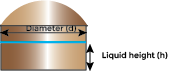
\includegraphics[scale=1]{DigesterWOCDimensions_1}
\end{center}

{
$=\dfrac
	{
		5000
		\dfrac
			{gal \enspace sludge}
			{day}
		*(8.34*0.06*0.66) 
		\dfrac
			{lbs VS}
			{gal \enspace  sludge}
	}
	{
		(\dfrac
			{\pi}
			{4}*37^2*27)ft^3
	}
=\boxed
	{
		0.057 \dfrac
			{lbs \enspace VS}
			{day-ft^3}
	}
$}

\item The sludge feed to a digester is 12,000 $ft^3$/day.  The sludge contains 4.5\% total solids with 70\% volatile solids.  What is the digester loading in lbs VSS/day per $ft^3$ if the digester diameter is 100 ft and a working sludge level of 20 ft.\\
	
Solution:\\
{
$
	Digester \enspace volatile \enspace solids 			\enspace loading \enspace Rate = 					\dfrac
	{
	Digester \enspace loading 
		\dfrac
		{
		lbs \enspace VS
		}
		{
		day
		}
	}
	{
	Digester \enspace volume (V)ft^3
	}
$
}\\

\begin{center}
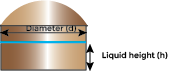
\includegraphics[scale=1]{DigesterWOCDimensions_1}
\end{center}

{
$=\dfrac
	{
		12,000
		\dfrac
			{
			ft^3 \enspace sludge
			}
			{
			day
			}
		*7.48 \dfrac
				{
				gal
				}
				{
				ft^3
				}	
		*(8.34*0.045*0.70) 
		\dfrac
			{lbs VS}
			{gal \enspace  sludge}
	}
	{
		(	\dfrac
			{
			\pi
			}
			{
			4
			}
			*100^2*20
		)
		ft^3
	}
=\boxed
	{
		0.15 \dfrac
			{
			lbs \enspace VS
			}
			{
			day-ft^3
			}
	}
$}\\
\item How much gas is produced in the above digester in $ft^3$/day if the digested sludge contains 2.5\% total solids of which 59\% is volatile solids and the gas production rate is 14 $ft^3$/lb VS destroyed?\\
Solution:\\

{
$
Digester \enspace VS \enspace reduction (\%)=
	\dfrac
	{0.70 - .59}
	{0.70 - 0.70 *0.59}
	*100=38.3\%
$
}\\
\vspace{6mm}

{
$
	\dfrac
	{
	lbs \enspace VS \enspace reduction
	}
	{
	day
	}
	=
	\dfrac
	{
	3153 lbs \enspace VS \enspace feed
		*  0.383 \enspace VS \enspace reduction
	}
	{
	day
	}
 	=1,208
	\dfrac
	{
	lbs \enspace VS \enspace reduction
	}
	{
	day 
	}
$
}\\
\vspace{6mm}

{
$
	\dfrac 
	{
	ft^3 gas \enspace produced
	}
	{
	day
	}
	=
	1208 \dfrac
			{
			lbs \enspace VS \enspace reduced
			}
			{
			day
			}
			*
		\dfrac
		{
		14 ft^3 \enspace gas \enspace produced
		}
		{
		lb \enspace VS \enspace reduced
		}
		=16,912 \dfrac
				{
				ft^3 \enspace digester \enspace 					gas \enspace produced
				}
				{
				day
				}
$
} 
\item The sludge feed to a digester is 80,000 gal/day. The sludge contains 4.5\% total solids with 75\% volatile solids. If 50\% of VS are reduced in the digester: 



\begin{enumerate}
\item Find lbs VS destroyed per 1000 gal of digester capacity per day if the digester radius is 55 ft with an operating sludge level of 25 ft.(5 points)

\vspace{1cm}
Solution:\\
Digester Volume: 
$
{
		(\pi*55^2*25)ft^3 *7.48 \dfrac{gal}{ft^3}
	}=1,776,220 gallons=1,776.2 \enspace(1000 \enspace gallons)
$
\\
\vspace{3mm}
$
	\dfrac
	{
	lbs \enspace VS \enspace reduction
	}
	{
	day
	}
	=
	\dfrac
	{
	80,000 gal * 8.34 \dfrac{lbs}{gal}*(0.045*0.75) \dfrac{lbs VS}{lb}*0.5\dfrac{lbs \enspace VS \enspace  reduction}{lb \enspace VS}
	}
	{
	day
	}$\\
\vspace{0.5cm}
$
 	=11,259
	\dfrac
	{
	lbs \enspace VS \enspace reduction
	}
	{
	day 
	}
$
\\
\vspace{3mm}


$
	\dfrac
	{
	lbs \enspace VS \enspace reduction
	}
	{
	1000 \enspace digester \enspace capacity
	}
	=
	\dfrac
	{
	11,259 \dfrac
			{
			lbs \enspace VS \enspace reduction
			}
			{
			day
			}
	}
	{	
	1,776.2 \enspace (1000 \enspace gallons)
	}
 	=\boxed{6.3
	\dfrac
	{
	lbs \enspace VS \enspace reduction
	}
	{
	1000 gallons \enspace digester \enspace volume 
	}}
$
\\

\vspace{1cm}

\item  What is the digester gas production in Btu/day? Assume 14 cu. ft digester gas per lb of VS destroyed and a 650 Btu/cu. ft heating value for the digester gas produced (5 points)
\end{enumerate}
\vspace{1cm}
Solution:\\

$
	\dfrac 
	{
	ft^3 gas \enspace produced
	}
	{
	day
	}
	=
	11,259 \dfrac
			{
			lbs \enspace VS \enspace reduced
			}
			{
			day
			}
			*
		\dfrac
		{
		14 ft^3 \enspace gas \enspace produced
		}
		{
		lb \enspace VS \enspace reduced
		}
		=157,626 \dfrac
				{
				ft^3 \enspace digester \enspace 					gas \enspace produced
				}
				{
				day
				}
$
\\
\vspace{1cm}


$
	\dfrac 
	{
	BTU \enspace produced
	}
	{
	day
	}
	=
	157,626 \dfrac
			{
			ft^3 \enspace gas \enspace produced
			}
			{
			day
			}
			*
		\dfrac
		{
		650 BTU \enspace gas \enspace produced
		}
		{
		ft^3 gas
		}
		=\boxed{102,456,900 \dfrac
				{
				BTU \enspace produced
				}
				{
				day
				}}
$

\item Two sludges are blended together as follows: 15,000 gal. primary sludge at 4.1\% solids. 28,000 gal. secondary sludge at 1.3\% solids. What is the combined solids concentration?  If the primary sludge is 68\% VS and the secondary sludge is 63\% VS, what is the VS concentration (\%) in the combined sludge?

Solution:

Combined solids concentration:
$
C_1*V_1 + C_2*V_2 = C_3*V_3$\\
$\implies C_3 = \dfrac{C_1*V_1 + C_2*V_2}{V3}=\dfrac{C_1*V_1 + C_2*V_2}{V_1 + V_2}=\dfrac{4.1*15,000 + 1.3*28,000}{15,000 + 28,000}=\boxed{2.28\%}
$\\
Lbs of VS in combined sludge:
$
C\textsubscript{VS1}*V_1 + C\textsubscript{VS2}*V_2 = C\textsubscript{VS3}*V_3$\\
$\implies C\textsubscript{VS3} = \dfrac{C\textsubscript{VS1}*V_1 + C\textsubscript{VS2}*V_2}{V3}=\dfrac{C\textsubscript{VS1}*V_1 + C\textsubscript{VS1}*V_2}{V_1 + V_2}$\\
$\implies C\textsubscript{VS3}
=\dfrac{4.1*15,000*0.68 + 1.3*28,000*0.63}{15,000 + 28,000}=\boxed{1.50\%}$
\\


\item The volatile acids concentration of sludge in an anaerobic digester is 195 mg/l. If the maximum volatile acids:alkalinity ratio is 0.087, what should the alkalinity be in mg/l?\\
Solution:\\
Volatile acid:Alkalinity=0.087=$\dfrac{195}{x}\implies x = \dfrac{195}{0.087} =\boxed{2,241\dfrac{mg}{l}}$
\pagebreak
	
\item 10,000 gallons of sludge is pumped to an anaerobic digester/day at 4\% solids (70\% VS).  50\% of the VS are destroyed, creating 15 $ft^3$ of gas per lbs. of VS destroyed. How much gas is produced each day?\\

{
$
	\dfrac
	{
	lbs \enspace VS \enspace reduction
	}
	{
	day
	}
	=
	\dfrac
	{
	10,000 gal * 8.34 \dfrac{lbs}{gal}*(0.04*0.7) \dfrac{lbs VS}{lb}*\dfrac{0.5 lbs \enspace VS \enspace  reduction}{lb \enspace VS}
	}
	{
	day
	}
 	=1,168
	\dfrac
	{
	lbs \enspace VS \enspace reduction
	}
	{
	day 
	}
$
}\\
\vspace{3mm}

{
$
	\dfrac 
	{
	ft^3 gas \enspace produced
	}
	{
	day
	}
	=
	1,168 \dfrac
			{
			lbs \enspace VS \enspace reduced
			}
			{
			day
			}
			*
		\dfrac
		{
		15 ft^3 \enspace gas \enspace produced
		}
		{
		lb \enspace VS \enspace reduced
		}
		=17,520 \dfrac
				{
				ft^3 \enspace digester \enspace 					gas \enspace produced
				}
				{
				day
				}
$
} 


\item Given a sludge flow of 5,500 gpd with 6.5\% solids containing  72\% VS to a digester with a VS destruction of 48\%   If the digester is digester is 40 ft. diameter with a sludge level of 25 ft, find lbs. VS destroyed per 1000 gal of digester capacity per day.  What is the digester gas production in Btu/day if the \% VS reduction in the digester is 58\% and the digester raw sludge feed is 6000 cu. Ft/day containing 4.5\% total solids with a 64\% VS content?  Assume 13.5 cu. ft digester gas per lb of VS destroyed and a 650 Btu/cu. ft heating value for the digester gas produced\\

{
Digester Volume: 
$
{
		(\dfrac
			{\pi}
			{4}*40^2*25)ft^3 *7.48 \dfrac{gal}{ft^3}
	}=940,086 gallons=940 \enspace(1000 \enspace gallons)
$
}\\
\vspace{3mm}

{
$
	\dfrac
	{
	lbs \enspace VS \enspace reduction
	}
	{
	day
	}
	=
	\dfrac
	{
	5,500 gal * 8.34 \dfrac{lbs}{gal}*(0.065*0.72) \dfrac{lbs VS}{lb}*\dfrac{0.48 lbs \enspace VS \enspace  reduction}{lb \enspace VS}
	}
	{
	day
	}
 	=1,030
	\dfrac
	{
	lbs \enspace VS \enspace reduction
	}
	{
	day 
	}
$
}\\
\vspace{3mm}


{
$
	\dfrac
	{
	lbs \enspace VS \enspace reduction
	}
	{
	1000 \enspace digester \enspace capacity
	}
	=
	\dfrac
	{
	1,030 \dfrac
			{
			lbs \enspace VS \enspace reduction
			}
			{
			day
			}
	}
	{	
	940 \enspace (1000 \enspace gallons)
	}
 	=1.1
	\dfrac
	{
	lbs \enspace VS \enspace reduction
	}
	{
	1000 gallons \enspace digester \enspace volume 
	}
$
}\\
\vspace{3mm}


{
$
	\dfrac 
	{
	ft^3 gas \enspace produced
	}
	{
	day
	}
	=
	1,030 \dfrac
			{
			lbs \enspace VS \enspace reduced
			}
			{
			day
			}
			*
		\dfrac
		{
		13.5 ft^3 \enspace gas \enspace produced
		}
		{
		lb \enspace VS \enspace reduced
		}
		=13,905 \dfrac
				{
				ft^3 \enspace digester \enspace 					gas \enspace produced
				}
				{
				day
				}
$
}\\
\vspace{3mm}



{
$
	\dfrac 
	{
	BTU \enspace produced
	}
	{
	day
	}
	=
	13,905 \dfrac
			{
			ft^3 \enspace gas \enspace produced
			}
			{
			day
			}
			*
		\dfrac
		{
		650 BTU \enspace gas \enspace produced
		}
		{
		ft^3 gas
		}
		=9,038,250 \dfrac
				{
				BTU \enspace produced
				}
				{
				day
				}
$
}

\item Two sludges are blended together as follows: 60,000 gal per day. primary sludge at 4.5\% solids and 28,000 gal secondary sludge at 5\% solids. 
\begin{enumerate}
\item What is the combined solids concentration?  (3 points)\\

$\dfrac{60,000*4.5+28,000*5}{88,000}=\boxed{4.66\%}$\\
\vspace{2cm}
\item How many lbs of solids (per day) are in the combined sludge (3 points)\\

$88,000 gal*8.34*0.0466 = \boxed{34,200 lbs}$\\
\vspace{2cm}


\item If the primary sludge is 68\% VS and the secondary sludge is 83\% VS, how many pounds of VS are in the combined sludge? (3 points)\\
$60,000 gal *\dfrac{8.34*0.045*0.68lbs \enspace VS}{gal}+28,000 gal *\dfrac{8.34*0.05*0.83lbs \enspace VS}{gal}=\boxed{25,003 lbs \enspace VS}$
\vspace{2cm}

\item What is the digester feed VS\%?  (3 points)\\
$\dfrac{25,003 lbs \enspace VS}{34,200 lbs TS}=\boxed{73.1\%}$

\vspace{2cm}



\item If the digester is 120’ diameter with a liquid height of 20’, what is the VS loading in lbs VS/ft3-day (3 points)\\

$\dfrac{25,003 lbs \enspace VS}{0.785*120^2*20}=\boxed{\dfrac{0.11 lbs \enspace VS}{day-ft^3}}$\\
\vspace{2cm}





\item If the digested sludge has 52\% VS, calculate the digester VS reduction percent (3 points)\\

$
Digester \enspace VS \enspace reduction (\%)=
	\dfrac
	{0.731 - .52}
	{0.731 - 0.731 *0.52}
	*100=\boxed{60.1\%}
$\\
\vspace{2cm}

\item What is the gas production (ft$^3$/day) if the digester produces 14 ft$^3$ gas/lb VS destroyed (3 points)\\
25,003*0.601$\dfrac{lbs\enspace VS destroyed}{}*\dfrac{14ft^3 \enspace gas \enspace produced}{lb \enspace VS \enspace destroyed}=\boxed{210,375ft^3 gas}$
\\
\vspace{2cm}

\item How many belt presses are needed to keep up with the digested sludge flow if the belt presses can be operated at a maximum flow of 50 GPM (3 points)\\

88,000$\dfrac{gal \enspace sludge}{day}*\dfrac{day}{1440min}=61 GPM$\\
@50 GPM per press - $\boxed{2 \enspace BFP \enspace required}$
\vspace{2cm}
\item If the digested sludge feed to the belt filter presses is 2.6\% and assuming the belt press feed solids capture is 90\%.  How many lbs of solids (dry) are produced by the BFP (4 points)\\
$88,000\dfrac{gal}{day}*8.34*0.026\dfrac{lbs \enspace solids \enspace feed}{day}*0.9\dfrac{lbs \enspace solids \enspace captured}{lbs \enspace solids \enspace feed}=\boxed{17,174 lbs \enspace solids \enspace per \enspace day}$
\vspace{2cm}

\item If the BFP produces a 20\% cake, how many wet tons cake produced per day (4 points)\\
$\dfrac{17,174 lbs \enspace solids \enspace produced}{day}*\dfrac{100 lbs \enspace cake}{20 lbs \enspace solids \enspace produced}*\dfrac{tons}{2,000 lbs}=\boxed{\dfrac{42.9tons}{day}}$
\vspace{2cm}

\item If the cake density is 68 lbs/cu. ft, how much time will it take to fill a 30 cu. yd bin (3 points)\\
(Ans. 15.4 hours)
$\dfrac{(42.9*2000)lbs \enspace cake}{day}*\dfrac{day}{1440 min}=\dfrac{59.583}{lbs \enspace cake}{min}$\\
$\dfrac{59.583}{lbs \enspace cake}{min}*\dfrac{ft^3}{68 lbs \enspace cake}=\dfrac{0.876ft^3}{min}$\\
$30yd^3*\dfrac{27ft^3}{yd^3}*\dfrac{min}{0.876ft^3}*\dfrac{hrs}{60 min}=\boxed{15.4hrs}$
\vspace{2cm}
\item What will be the cost of hauling dewatered cake per day @ \$65 per ton cake (2 points)\\
42.9$\dfrac{tons}{day}*\dfrac{\$65}{ton}=\boxed{\dfrac{\$2,789}{day}}$ 
\end{enumerate}

\item Calculate the VS loading to the digester in lbs/day if 10,000 cu. ft of sludge containing 4.8\% TS with and an average VS content of 82\% 




\item Calculate the VS loading to the digester in lbs/day if 25,000 gallons of sludge containing 4.5\% TS with and average VS content of 76\% is fed to the digester 




\item Calculate the \% VS reduction in a digester given the volatile solids content of the feed sludge to the digester is 76\% and the volatile solids content of the sludge leaving the digester is 55\% 




\item Calculate the organic loading rate to two 320,000 gallon anaerobic digesters given:
Primary sludge feed rate of 25,000 gallons with 6.2\% TS containing 73\% solids and SG of 1.03.
Secondary sludge feed rate of 30,500 gallons with 3.8\% TS containing 77\% solids (7 points)
(Answer: 0.2lbs VS/day-ft3 ) 


\end{enumerate}
\textbf{Solving Dewatering Problems}
\begin{enumerate}
	\item \textbf{Calculation of solids recovery}\\
		\begin{enumerate}
		\item Calculate amount of solids fed to the dewatering unit
		\item Calculate the amount of solids produced as part of the dewatered cake
		\item The ratio of the solids in dewatered cake to that in the feed times 100 will give you the solids recovery (solids recovery rate)
		\end{enumerate}
	\item \textbf{Calculation of dewatered cake volume}\\
		\begin{enumerate}
		\item First calculate the amount of cake solids produced in terms of weight per time.
		\item From the weight of the cake produced calculate the volume - from the cake density which is normally given\\
		\end{enumerate}
	\item \textbf{Calculation of solids hauling costs or savings associated with change in cake solids content}\\
		\begin{enumerate}
		\item First calculate the amount of dry solids produced as part of the original wet cake solids percent
		\item Using the value of the dry solids calculate the wet cake weight with the new cake solids percentage\\
		\end{enumerate}
	\item \textbf{General formula for calculating net savings associated with change in cake solids content}\\
Savings =$ \dfrac {(New \enspace solids \enspace \%-Old \enspace Solids \enspace \%)}{New \enspace solids \enspace \%}*Old \enspace Cost$

So if the cake dryness goes up from 20\% to 26\% and currently a utility is spending \$ 1,000,000 per year for biosolids hauling and disposal, their net savings will be: (26\%-\%20)/26*\$ 1,000,000 = \$ 230,769
\end{enumerate}

\begin{enumerate}
\item Calculate the organic loading rate to two 320,000 gallon anaerobic digesters given:\\
Primary sludge feed rate of 25,000 gallons with 3.8\% TS containing 73\% solids and SG of 1.03.\\
Secondary sludge feed rate of 30,500 gallons with 3.8\% TS containing 77\% solids 
\\
(Answer: 0.2 $\dfrac{lbs \enspace VS}{day-ft^3}$)\\
\vspace{1cm}



\item 325 GPM of WAS with 7,000 mg/l TSS is thickened in a DAFT.  Assuming an air:solids ratio of 0.05 lb of air for each lb of feed solids, The SCFM (standard cubic feed per minute) air required to thicken the WAS given 1 SCFM = 0.075 lb is:\\
(Answer:  $12.6 \enspace SCFM$)\\
Solution:\\

Correct Answer:\\
$0.05=\dfrac{lb \enspace air}{lb \enspace solids}=\dfrac{\dfrac{0.075 \enspace lbs  \enspace air}{SCF}*x \enspace SCFM}{(\dfrac{325}{1,000,000}MG \enspace per \enspace min*7000*8.34) \enspace lbs  \enspace solids}$\\
\vspace{0.5cm}

$\implies x \enspace SCFM=\dfrac{0.05*325*7000*8.34}{0.075*1,000,000}=\boxed{12.6 \enspace SCFM} - Correct \enspace answer$\\
\vspace{0.5cm}
Incorrect Answer \#1:\\
12,600SCFM

\vspace{0.5cm}
Incorrect Answer \#2:\\
0.126SCFM


\vspace{0.5cm}
Incorrect Answer \#3:\\
1.26SCFM

\vspace{1cm}



\item 30,000 gpd of 4.5\% sludge is dewatered in a centrifuge yielding 24.5 $yd^3/day$ of 25\% cake with a density of 65 lb per $ft^3$.  Calculate the percentage solids recovery.\\
(Answer: 95.5\%)\\
\vspace{1cm}

\item Estimate the amount of heat value of the gas produced from an anaerobic digester in $\dfrac{BTU}{day}$ given the following: \\  
\renewcommand{\arraystretch}{0.6}
\begin{tabular}{ | m {7 cm} | m {4 cm}| } 
 \hline
Raw sludge pumping schedule & 12 min/hr \\ 
 \hline
Sludge pumping rate & 68 GPM\\ 
 \hline
 Raw sludge \%TS & 5.2\%  \\
 \hline
  Raw sludge \%VS & 72.5\%  \\
 \hline
Gas production & $\dfrac{12 ft^3}{lb \enspace VS \enspace destroyed \enspace - \enspace day}$\\
 \hline
 Percent $CO_2$ & 34\%\\ 
 \hline
 Other gases & 1\%  \\
 \hline
  Pure methane net heat value & 932 $\dfrac{BTU}{ft^3}$\\
 \hline
\end{tabular}\\
\vspace{0.3 cm}
(Answer: 23,146,220 $\dfrac{BTU}{day}$)

\item 12,000 $ft^3$ of anaerobically digested sludge containing 2.8\% TS is dewatered in a centrifuge.  The centrifuge yields 37 $yd^3$ of 26\% of dewatered cake with a density of 73 lb/$ft^3$.  Calculate the solids capture rate.\\


 

Solution:\\
$
	lbs \enspace TS \enspace feed \enspace to \enspace centrifuge
	=
	12,000 ft^3 \enspace sludge
	*
	7.48 
	\dfrac
	{
	gal
	}
	{
	ft^3
	}
	*
	\dfrac
	{
	(8.34*0.028 lbs \enspace TS )
	}
	{gal \enspace sludge
	}
	=20,960 {lbs \enspace TS}
$

$
	lbs \enspace TS \enspace feed \enspace from \enspace centrifuge
	=
	37 yd^3 \enspace sludge
	*
	27 
	\dfrac
	{
	ft^3
	}
	{
	yd^3
	}
	*
	\dfrac
	{
	(73 lbs *0.26 \enspace TS )
	}
	{ft^3 \enspace sludge
	}
	=18,961 {lbs \enspace TS}
$

$
	solids \enspace capture \enspace rate
	=
	\dfrac
	{
	18,961 lbs \enspace solids \enspace produced 		\enspace by \enspace centrifuge
	}
	{
	20,960 lbs \enspace solids \enspace fed 			\enspace from \enspace digester
	}
	*
	100 
	=\boxed
	{
	90.4\% solids \enspace capture
	}
$


\item At a 60 GPM of 2.8\% feed a belt press which has a 90\% solids capture rate produces a 20\% cake at 68 lbs/$ft^3$.  How long would it take to fill a 3 $yd^3$ bin  
	
	
Solution:\\
Approach:
\begin{itemize}
\item First calculate the amount of cake solids produced in terms of weight per time.
\item From the weight of the cake produced calculate the volume time, and finally
\item using the calculated value of the volume of the cake produced per time, calculate the time required to fill the bin\\
\end{itemize}

$\dfrac{cake \enspace TS \enspace produced - lbs}{min}= \dfrac {60 gallons \enspace sludge}{min}*\dfrac {8.34 lbs \enspace sludge \enspace feed}{galllon}*\dfrac{0.028 lbs \enspace TS}{lb \enspace sludge}*0.9$\\
\vspace{3mm}

$=\dfrac{12.61lbs \enspace TS}{min}$\\
\vspace{3mm}

$\dfrac{ft^3 \enspace cake \enspace produced}{min}=\dfrac{12.61lbs \enspace TS}{min}*\dfrac{100 lbs \enspace cake}{20lbs \enspace TS}*\dfrac{ft^3 \enspace cake}{68 lbs \enspace cake} = \dfrac{0.927ft^3 cake}{min}$\\
\vspace{3mm}

$\dfrac{ft^3 \enspace cake \enspace produced}{min}=\dfrac{12.61lbs \enspace TS}{min}*\dfrac{100 lbs \enspace cake}{20lbs \enspace TS}*\dfrac{ft^3 \enspace cake}{68 lbs \enspace cake} = \dfrac{0.927ft^3 cake}{min}$\\
\vspace{3mm}
$Time \enspace required \enspace to \enspace fill \enspace the \enspace bin=\dfrac{min}{0.927ft^3}*{3yd^3}*\dfrac{27ft^3}{yd^3}=\boxed{75min}$\\
\pagebreak
\item Calculate the annual cost savings for an improvement of cake solids from 20\% to 21\% if 400 wet tons (@ 20\% cake) are produced each day and the average cake hauling and disposal cost is \$65 per wet ton.\\
$Total \enspace (dry)\enspace solids \enspace produced \enspace per \enspace day =\dfrac{400 \enspace wet \enspace tons}{day}*\dfrac{20 tons \enspace solids}{100 wet \enspace tons}={80 tons \enspace solids}$\\
\vspace{3mm}
$Tons \enspace wet \enspace cake \enspace@ 21\% \enspace solids =\dfrac{80 \enspace tons \enspace solids}{day}*\dfrac{100 wet \enspace tons}{21 tons \enspace solids}$

\vspace{3mm}
$=\dfrac{380 tons \enspace  wet \enspace solids}{day}$\\
\vspace{3mm}
$Net \enspace savings \enspace (\$/yr) = (400 - 380)\dfrac{wet \enspace tons}{day}*365*\dfrac{days}{yr}*\dfrac{\$65}{wet \enspace ton}=\boxed{\$474,500 \enspace per \enspace year}$


\textbf {NOTE:  General formula for future reference: So if the cake dryness goes up from 20\% to 26\% and currently a utility is spending \$1,000,000 per year for biosolids hauling and disposal, their net savings will be: (26-20)/26*1,000,000 = \$230,769.  Conversely say if the dewatering cake solids drops to 18\%, the net impact will be: (18-20)/18*1,000,000 = \$-111,111 (loss or extra cost).}
\\

\item Two sludges are blended together as follows: 60,000 gal per day. primary sludge at 4.5\% solids and 28,000 gal secondary sludge at 5\% solids. 
\begin{enumerate}
\item What is the combined solids concentration?  (3 points)\\

$\dfrac{60,000*4.5+28,000*5}{88,000}=\boxed{4.66\%}$\\
\vspace{0.5cm}
\item How many lbs of solids (per day) are in the combined sludge (3 points)\\

$88,000 gal*8.34*0.0466 = \boxed{34,200 lbs}$\\
\vspace{0.5cm}


\item If the primary sludge is 68\% VS and the secondary sludge is 83\% VS, how many pounds of VS are in the combined sludge? (3 points)\\
$60,000 gal *\dfrac{8.34*0.045*0.68lbs \enspace VS}{gal}+28,000 gal *\dfrac{8.34*0.05*0.83lbs \enspace VS}{gal}=\boxed{25,003 lbs \enspace VS}$
\vspace{2cm}

\item What is the digester feed VS\%?  (3 points)\\
$\dfrac{25,003 lbs \enspace VS}{34,200 lbs TS}=\boxed{73.1\%}$
\vspace{0.5cm}

\item If the digester is 120’ diameter with a liquid height of 20’, what is the VS loading in lbs VS/ft3-day (3 points)\\

$\dfrac{25,003 lbs \enspace VS}{0.785*120^2*20}=\boxed{\dfrac{0.11 lbs \enspace VS}{day-ft^3}}$\\
\vspace{0.5cm}

\item If the digested sludge has 52\% VS, calculate the digester VS reduction percent (3 points)\\

$
Digester \enspace VS \enspace reduction (\%)=
	\dfrac
	{0.731 - .52}
	{0.731 - 0.731 *0.52}
	*100=\boxed{60.1\%}
$\\
\vspace{0.5cm}

\item What is the gas production (ft$^3$/day) if the digester produces 14 ft$^3$ gas/lb VS destroyed (3 points)\\
25,003*0.601$\dfrac{lbs\enspace VS destroyed}{}*\dfrac{14ft^3 \enspace gas \enspace produced}{lb \enspace VS \enspace destroyed}=\boxed{210,375ft^3 gas}$
\\
\vspace{0.5cm}

\item How many belt presses are needed to keep up with the digested sludge flow if the belt presses can be operated at a maximum flow of 50 GPM (3 points)\\

88,000$\dfrac{gal \enspace sludge}{day}*\dfrac{day}{1440min}=61 GPM$\\
@50 GPM per press - $\boxed{2 \enspace BFP \enspace required}$
\vspace{0.5cm}
\item If the digested sludge feed to the belt filter presses is 2.6\% and assuming the belt press feed solids capture is 90\%.  How many lbs of solids (dry) are produced by the BFP (4 points)\\
$88,000\dfrac{gal}{day}*8.34*0.026\dfrac{lbs \enspace solids \enspace feed}{day}*0.9\dfrac{lbs \enspace solids \enspace captured}{lbs \enspace solids \enspace feed}=\boxed{17,174 lbs \enspace solids \enspace per \enspace day}$
\vspace{0.5cm}

\item If the BFP produces a 20\% cake, how many wet tons cake produced per day (4 points)\\
$\dfrac{17,174 lbs \enspace solids \enspace produced}{day}*\dfrac{100 lbs \enspace cake}{20 lbs \enspace solids \enspace produced}*\dfrac{tons}{2,000 lbs}=\boxed{\dfrac{42.9tons}{day}}$
\vspace{0.5cm}

\item If the cake density is 68 lbs/cu. ft, how much time will it take to fill a 30 cu. yd bin (3 points)\\
(Ans. 15.4 hours)
$\dfrac{(42.9*2000)lbs \enspace cake}{day}*\dfrac{day}{1440 min}=\dfrac{59.583}{lbs \enspace cake}{min}$\\
$\dfrac{59.583}{lbs \enspace cake}{min}*\dfrac{ft^3}{68 lbs \enspace cake}=\dfrac{0.876ft^3}{min}$\\
$30yd^3*\dfrac{27ft^3}{yd^3}*\dfrac{min}{0.876ft^3}*\dfrac{hrs}{60 min}=\boxed{15.4hrs}$
\vspace{0.5cm}
\item What will be the cost of hauling dewatered cake per day @ \$65 per ton cake (2 points)\\
42.9$\dfrac{tons}{day}*\dfrac{\$65}{ton}=\boxed{\dfrac{\$2,789}{day}}$
\end{enumerate}

\item 12,000 $ft^3$ of anaerobically digested sludge containing 2.8\% TS is dewatered in a centrifuge.  The centrifuge yields 37 $yd^3$ of 26\% of dewatered cake with a density of 73 lb/$ft^3$.  Calculate the solids capture rate.\\


 

Solution:\\
{
$
	lbs \enspace TS \enspace feed \enspace to \enspace centrifuge
	=
	12,000 ft^3 \enspace sludge
	*
	7.48 
	\dfrac
	{
	gal
	}
	{
	ft^3
	}
	*
	\dfrac
	{
	(8.34*0.028 lbs \enspace TS )
	}
	{gal \enspace sludge
	}
	=20,976 {lbs \enspace TS}
$
}

{
$
	lbs \enspace TS \enspace feed \enspace from \enspace centrifuge
	=
	37 yd^3 \enspace sludge
	*
	27 
	\dfrac
	{
	ft^3
	}
	{
	yd^3
	}
	*
	\dfrac
	{
	(73 lbs *0.26 \enspace TS )
	}
	{ft^3 \enspace sludge
	}
	=18,961 {lbs \enspace TS}
$
}

{
$
	solids \enspace capture \enspace rate
	=
	\dfrac
	{
	18,961 lbs \enspace solids \enspace produced 		\enspace by \enspace centrifuge
	}
	{
	20,976 lbs \enspace solids \enspace fed 			\enspace from \enspace digester
	}
	*
	100 
	=\boxed
	{
	90.4\% solids \enspace capture
	}
$
}

\item At a 60 GPM of 2.8\% feed a belt press which has a 90\% solids capture rate produces a 20\% cake at 68 lbs/$ft^3$.  How long would it take to fill a 3 $yd^3$ bin  
	
	
Solution:\\
Approach:
\begin{itemize}
\item First calculate the amount of cake solids produced in terms of weight per time.
\item From the weight of the cake produced calculate the volume time, and finally
\item using the calculated value of the volume of the cake produced per time, calculate the time required to fill the bin\\
\end{itemize}

{$\dfrac{cake \enspace TS \enspace produced - lbs}{min}= \dfrac {60 gallons \enspace sludge}{min}*\dfrac {8.34 lbs \enspace sludge \enspace feed}{galllon}*\dfrac{0.028 lbs \enspace TS}{lb \enspace sludge}*0.9$}\\
\vspace{3mm}

{$=\dfrac{12.61lbs \enspace TS}{min}$}\\
\vspace{3mm}

{$\dfrac{ft^3 \enspace cake \enspace produced}{min}=\dfrac{12.61lbs \enspace TS}{min}*\dfrac{100 lbs \enspace cake}{20lbs \enspace TS}*\dfrac{ft^3 \enspace cake}{68 lbs \enspace cake} = \dfrac{0.927ft^3 cake}{min}$}\\
\vspace{3mm}

{$\dfrac{ft^3 \enspace cake \enspace produced}{min}=\dfrac{12.61lbs \enspace TS}{min}*\dfrac{100 lbs \enspace cake}{20lbs \enspace TS}*\dfrac{ft^3 \enspace cake}{68 lbs \enspace cake} = \dfrac{0.927ft^3 cake}{min}$}\\
\vspace{3mm}

{$Time \enspace required \enspace to \enspace fill \enspace the \enspace bin=\dfrac{min}{0.927ft^3}*{3yd^3}*\dfrac{27ft^3}{yd^3}=\boxed{75min}$}\\
\pagebreak
\item Calculate the annual cost savings for an improvement of cake solids from 20\% to 21\% if 400 wet tons (@ 20\% cake) are produced each day and the average cake hauling and disposal cost is \$65 per wet ton.\\
Solution:\\
{$Total \enspace (dry)\enspace solids \enspace produced \enspace per \enspace day =\dfrac{400 \enspace wet \enspace tons}{day}*\dfrac{20  \enspace tons \enspace solids}{100  \enspace wet \enspace tons}={80  \enspace tons \enspace solids}$}\\
\vspace{3mm}
{$Tons \enspace wet \enspace cake \enspace@ 21\% \enspace solids =\dfrac{80 \enspace tons \enspace solids}{day}*\dfrac{100  \enspace wet \enspace tons}{21  \enspace tons \enspace solids}$}

\vspace{3mm}
{$=\dfrac{380  \enspace tons \enspace  wet \enspace solids}{day}$}\\
\vspace{3mm}
{$Net \enspace savings \enspace (\$/yr) = (400 - 380)\dfrac{wet \enspace tons}{day}*365*\dfrac{days}{yr}*\dfrac{\$65}{wet \enspace ton}=\boxed{\$474,500 \enspace per  \enspace year}$}


\textbf {NOTE:  General formula for future reference: So if the cake dryness goes up from 20\% to 26\% and currently a utility is spending \$1,000,000 per year for biosolids hauling and disposal, their net savings will be: $\dfrac{(26-20)}{20}*\$1,000,000 = \$300,000$}
\\
\item A belt press is used for dewatering 70 GPM digested sludge containing 3\% TS, seven hours per day.  At the end of the day it produces 24 $yd^3$ of 16\% TS \enspace biosolids @ 65 lbs/$ft^3$ density.  What is the percent belt press solids recovery?\\
Solution:\\
lbs solids feed to belt press:  $\dfrac{70 \enspace gal}{min}*\dfrac{8.34 \enspace lbs}{gal}*
\dfrac{0.03 \enspace lbs \enspace solids}{lb \enspace feed \enspace sludge}*\dfrac{7*60 \enspace min}{day}=\dfrac{7,356 \enspace lbs \enspace solids}{day}$\\
\vspace{0.5cm}
lbs solids in belt press cake: $\dfrac{24 \enspace yd^3 \enspace cake}{day}*\dfrac{27 \enspace ft^3}{yd^3}*\dfrac{65 \enspace lbs \enspace cake}{ft^3}*\dfrac{0.16 \enspace lbs \enspace solids}{lb \enspace cake}=\dfrac{6,739 \enspace lbs \enspace solids}{day}$\\
\vspace{0.5cm}
belt press solids recovery: $\dfrac{6,739}{7,356}=\boxed{0.92 \enspace or \enspace 92\%}$


\item Calculate the air required (SCFM) to meet a 0.04 lb air:lb feed solids ratio for a 100 GPM WAS flow with a solids content of 6500mg/l? Assume 0.08 lbs air/SCF air.\\
Solution:\\
$0.04=\dfrac{lb \enspace air}{lb \enspace solids}=\dfrac{\dfrac{0.08 \enspace lbs  \enspace air}{SCF}*x \enspace SCF \enspace per \enspace  minute}{(\dfrac{100}{1,000,000}MG \enspace per \enspace min*6500mg/l*8.34) \enspace lbs  \enspace solids}$\\
\vspace{0.5cm}
$\implies0.04=0.0148 \enspace *\enspace x \enspace SCF \enspace per \enspace  minute \implies x \enspace SCF \enspace per \enspace  minute =\dfrac{0.04}{0.0148}=\boxed{2.7 \enspace SCFM}$

\item A treatment plant receives an influent flow of 30 MGD with a TSS concentration of 280 mg/l.  The primary treatment removes 55\% TS and the primary sludge is pumped to a 40 ft diameter gravity thickener.  Calculate the average solids loading to the thickener in lbs TSS/day-ft$^2$\\
Solution:\\
 
Solids loading to gravity thickener=$\dfrac{(30 \enspace MGD \enspace * \enspace 280*0.55 \enspace mg/l \enspace *8.34) lbs \enspace TSS \enspace per  \enspace day}{0.785*40^2 \enspace ft^2}=\boxed{30.7 \enspace lbs TSS/day-ft^2}$
\pagebreak
\item Two, 110' diameter digesters with a cone depth of 15 ft and operating at a cylindrical liquid level of 28 ft is fed with a blend of primary and secondary sludge.  The 85,000 gal/day primary sludge feed contains 5\% solids with a 65\% VS content.  The secondary sludge flow is 33,000 gallons per day with a 5.5\% solids and 86\% VS content.  

\begin{enumerate}
\item What is the combined solids concentration?\\
Combined solids concentration:\\
$
C_1*V_1 + C_2*V_2 = C_3*V_3$\\
$\implies C_3 = \dfrac{C_1*V_1 + C_2*V_2}{V3}=\dfrac{C_1*V_1 + C_2*V_2}{V_1 + V_2}=\dfrac{5*85,000 + 5.5*33,000}{88,000 + 33,000}=\boxed{5.14\% \enspace TS \enspace content}
$\\

\item What is the digester VS loading rate ($lbs \enspace VS / ft^3$)\\
Digester VS loading = $\dfrac{lbs \enspace VS}{Digester \enspace volume}$\\
\vspace{0.3cm}
$\implies \dfrac{8.34*(Pri. \enspace Sldg \enspace gal/day *Pri. Sldg \enspace TS *\%VS + \enspace Sec. \enspace sludge \enspace gal/day *Sec. \enspace sludge TS *\%VS)}{2*\Big[\dfrac{3.14*D^2*h_1}{12}+0.785*D^2*h\Big]}$
 \vspace{0.4cm}
 
 
 
$\implies \dfrac{8.34*(88,000 \enspace gal/day *0.05*0.65 \enspace+ \enspace 33,000 \enspace gal/day *0.055*0.86)}{2*\Big[\dfrac{(3.14*110^2*15}{12}+0.785*110^2*28\Big]}$
 \vspace{0.4cm}
$=\boxed{0.059 \dfrac{lbs \enspace VS}{ft^3}}$
\vspace{0.4cm}
\item If the digested sludge has 52\% VS, calculate the digester VS reduction percent\\
\vspace{0.4cm}
Calculate VS\% in: $=\dfrac{lbs \enspace VS}{lbs \enspace TS}*100$\\
$\implies \dfrac{8.34*(Pri. \enspace Sldg \enspace gal/day *Pri. Sldg \enspace TS *\%VS + \enspace Sec. \enspace sludge \enspace gal/day *Sec. \enspace sludge TS *\%VS)}{8.34*(Pri. \enspace Sldg \enspace gal/day *Pri. Sldg \enspace TS  + \enspace Sec. \enspace sludge \enspace gal/day *Sec. \enspace sludge TS *)}$\\
 \vspace{0.4cm}
$\implies \dfrac{8.34*(88,000 \enspace gal/day *0.05*0.65 \enspace+ \enspace 33,000 \enspace gal/day *0.055*0.86)}{8.34*(88,000 \enspace gal/day *0.05\enspace+ \enspace 33,000 \enspace gal/day *0.055)}*100$\\
\vspace{0.4cm}
$=\frac{36,870 lbs \enspace VS}{51,833 \enspace lbs \enspace TS}*100=\boxed{71.1 \% VS_{in}}$

$
Digester \enspace VS \enspace reduction (\%)=
	\dfrac
	{0.71 - .52}
	{0.71 - 0.71 *0.52}
	*100=\boxed{55.8\% \enspace VS \enspace reduction}
$\\
\vspace{0.5cm}

\item What is the gas production (ft$^3$/day) if the digester produces 14 ft$^3$ gas/lb VS destroyed\\
$36,870 \enspace lbs \enspace VS_{in}*0.558 lbs\enspace VS \enspace destroyed*\dfrac{14ft^3 \enspace gas \enspace produced}{lb \enspace VS \enspace destroyed}=\boxed{288,028 \enspace ft^3 \enspace gas \enspace produced}$
\\
\vspace{0.4cm}
\item \item How many belt presses are needed to keep up with the digested sludge flow if the belt presses can be operated at a maximum flow of 50 GPM \\

121,000$\dfrac{gal \enspace sludge}{day}*\dfrac{day}{1440min}=84 GPM$\\
@50 GPM per press - $\boxed{2 \enspace BFP \enspace required}$

\item If the digested sludge feed to the belt filter presses is 2.6\% and assuming the belt press feed solids capture is 90\%.  How many lbs of solids (dry) are produced by the BFP \\
$121,000\dfrac{gal}{day}*8.34*0.026\dfrac{lbs \enspace solids \enspace feed}{day}*0.9\dfrac{lbs \enspace solids \enspace captured}{lbs \enspace solids \enspace feed}=\boxed{23,028 lbs \enspace solids \enspace per \enspace day}$

\item If the belt press produces a 20\% cake at 68 lbs/$ft^3$.  How long would it take to fill a 3 $yd^3$ bin?
\vspace{0.3cm}

$lbs \enspace cake: 23,028 \enspace \dfrac{lbs \enspace solids}{day}*\dfrac{lb \enspace cake}{0.2 \enspace lb \enspace solids}=115,140 \enspace \dfrac{lbs \enspace cake}{day}$\\

\vspace{0.3cm}
Volume of cake produced: $115,140 \enspace \dfrac{lbs \enspace cake}{day}*\dfrac{ft^3}{68 \enspace lbs \enspace cake}*\dfrac{yd^3}{27 \enspace ft^3}*\dfrac{day}{24 \enspace hrs} =2.61 \enspace \dfrac{yd^3 \enspace cake}{hr}$
\item Time to fill the 3 cu. yd bin: $3 \enspace yd^3 *\dfrac{hr}{2.61 yd^3 \enspace cake}=\boxed{1.15 \enspace hrs}$

 
\end{enumerate}

eak
\item Two sludges are blended together as follows: 60,000 gal. primary sludge at 4.5\% solids and 28,000 gal. secondary sludge at 5\% solids. 
\begin{enumerate}
\item What is the combined solids concentration? 
\item If the primary sludge is 68\% VS and the secondary sludge is 83\% VS, how many pounds of VS are in the combined sludge? 
\item If the digester is 120’ diameter cylinder with a liquid height of 20’, what is the VS loading in lbs VS/$ft^3$-day?
\item If the digester VS reduction is 60\%, what is the gas production ($ft^3$/day) if the digester produces 14 $ft^3$ gas/lb VS destroyed?
\item How many belt presses are needed to keep up with the digested sludge flow if the belt presses are operated at a maximum flow of 50 GPM ?
\item Knowing the digester VS reduction and the TS feed, calculate the solids (TS) concentration coming out of the digesters
\item Assuming the belt press solids capture is 90\%; if it produces a 20\% cake which is 68 lbs/$ft^3$, in how many hours will it take to fill a 3 $yd^3$ bin with the cake?
\end{enumerate}
Solution:\\
\begin{enumerate}
\item What is the combined solids concentration?\\
Combined solids concentration:
$
C_1*V_1 + C_2*V_2 = C_3*V_3$\\
$\implies C_3 = \dfrac{C_1*V_1 + C_2*V_2}{V3}=\dfrac{C_1*V_1 + C_2*V_2}{V_1 + V_2}=\dfrac{4.5*60,000 + 5*28,000}{60,000 + 28,000}=\boxed{4.66\%}
$\\

lbs TS from primary sludge: $(4.5*10,000)\dfrac{mg}{l}TS*\dfrac{60,000}{1,000,000}MGD*8.34=22,518 \enspace lbs \enspace TS$\\
lbs TS from secondary sludge: $(5*10,000)\dfrac{mg}{l}TS*\dfrac{28,000}{1,000,000}MGD*8.34=11,676 \enspace lbs \enspace TS$\\
Total TS = 22,518+11,676=34,194 lbs TS\\
$TS \enspace conc.(mg/l) = \dfrac{34,194 \enspace lbs \enspace TS}{8.34*\dfrac{88,000}{1,000,000}MGD}=\boxed{46,591\dfrac{mg}{l} \enspace or \enspace 4.66\%}$

\item If the primary sludge is 68\% VS and the secondary sludge is 83\% VS, how many pounds of VS are in the combined sludge?\\
lbs of VS in combined sludge:
$
C\textsubscript{VS1}*V_1 + C\textsubscript{VS2}*V_2 = C\textsubscript{VS3}*V_3$\\
$\implies C\textsubscript{VS3} = \dfrac{C\textsubscript{VS1}*V_1 + C\textsubscript{VS2}*V_2}{V3}=\dfrac{C\textsubscript{VS1}*V_1 + C\textsubscript{VS1}*V_2}{V_1 + V_2}$\\
$\implies C\textsubscript{VS3}
=\dfrac{4.5*60,000*0.68 + 5*28,000*0.83}{60,000 + 28,000}=3.406\%$\\
$lbs \enspace VS=3.41*10,000 mg/l * \dfrac{88,000}{1,000,000}*8.34=\boxed{25,027 \enspace lbs \enspace VS}$\\


lbs VS from primary sludge: $(4.5*0.68*10,000)\dfrac{mg}{l}VS*\dfrac{60,000}{1,000,000}MGD*8.34=15,312 \enspace lbs \enspace VS$
lbs VS from secondary sludge: $(5*0.83*10,000)\dfrac{mg}{l}VS*\dfrac{28,000}{1,000,000}MGD*8.34=9,691 \enspace lbs \enspace VS$
Total VS = 15,312+9,691=$\boxed{25,003 \enspace lbs \enspace VS}$

\item If the digester is 120’ diameter cylinder with a liquid height of 20’, what is the VS loading in lbs VS/$ft^3$-day?

$VS \enspace loading=\dfrac{lbs \enspace VS \enspace per-day}{Digester \enspace volume \enspace (ft^3)}=\dfrac{25,003 \enspace lbs \enspace VS \enspace per-day}{0.785*120^2*20 \enspace ft^3}=\boxed{\dfrac{0.11 \enspace lbs \enspace VS}{day-ft^3}}$

\item If the digester VS reduction is 60\%, what is the gas production ($ft^3$/day) if the digester produces 14 $ft^3$ gas/lb VS destroyed?\\
$Digester \enspace gas \enspace production = lbs \enspace VS \enspace reduced * gas \enspace production \enspace rate (ft^3/lb \enspace lbs \enspace VS \enspace reduced$
$\implies 25,003*0.6 \enspace lbs \enspace VS reduced*\dfrac{14 \enspace ft^3 \enspace gas}{lb \enspace VS \enspace destroyed}=\boxed{210,025 \enspace ft^3 \enspace gas \enspace per-day}$

\item How many belt presses are needed to keep up with the digested sludge flow if the belt presses are operated at a maximum flow of 50 GPM?\\
Flow to the belt press=Flow to the digesters as digesters are fixed volume tanks\\
$\implies$ flow in to the digester = flow out of the digesters - which will be the flow to the belt press\\
$\implies$ flow to the belt press = 88,000 gal
$\implies 88,000 \dfrac{gal}{day}*\dfrac{day}{1440 \enspace min}= 61 \dfrac{gal}{min}$\\
$\implies @ 50 \enspace GPM \enspace belt \enspace press \enspace flow \enspace capacity \enspace need \enspace \boxed{2 \enspace belt \enspace presses}$
\pagebreak
\item Knowing the digester VS reduction and the TS feed, calculate the solids (TS) concentration coming out of the digesters\\
Approach:  Calculate the lbs of VS destroyed in the digester and subtract that out of the lbs TS feed to the digester.  This will be the mass of solids leaving the digester.  The mass of solids divided by the volume of the feed (also the out) would be the TS concentration\\

\vspace{0.5cm}

$\implies \dfrac{34,194 \enspace lbs \enspace TS \enspace feed - 25,003*0.6 \enspace lbs \enspace VS \enspace reduced}{88,000 \enspace gal*8.34 \enspace \dfrac{lbs}{gal}*\dfrac{10^6lbs}{1,000,000lbs}}$\\
\vspace{0.5cm}
$=20,441\dfrac{lbs \enspace solids}{10^6 \enspace lbs} \enspace or \enspace 26,150 \enspace ppm \enspace or \enspace \boxed{2.61\%} $


\item Assuming the belt press solids capture is 90\%; if it produces a 20\% cake which is 68 lbs/$ft^3$, in how many hours will it take to fill a 3 $yd^3$ bin with the cake?\\
Approach\\
\begin{enumerate}
\item Calculate the lbs of solids feed to the belt press. \item Based on the 90\% capture rate, calculate the lbs of solids leaving the belt press.  \item Knowing the cake is 20\% solids, calculate the lbs of cake produced. \item Knowing the density of the cake (68 lbs/$ft^3$), calculate the volume of the cake produced. \item Knowing the cake volume produced, calculate the time it will take to fill the 3 cu. yd bin\end{enumerate}

Calculations:\\
\begin{enumerate}
\item $(34,194 \enspace lbs \enspace TS \enspace feed - 25,003*0.6 \enspace lbs \enspace VS \enspace reduced)\enspace solids \enspace feed \enspace belt \enspace press$\\
$=19,192 \enspace lbs \enspace TS \enspace solids \enspace feed$\\
\item solids leaving belt press: 19,192*0.9=17,273 lbs\\
\item $lbs \enspace cake: 17,273 \enspace \dfrac{lbs \enspace solids}{day}*\dfrac{lb \enspace cake}{0.2 \enspace lb \enspace solids}=86,365 \enspace \dfrac{lbs \enspace cake}{day}$\\
\item Volume of cake produced: $86,365 \enspace \dfrac{lbs \enspace cake}{day}*\dfrac{ft^3}{68 \enspace lbs \enspace cake}*\dfrac{yd^3}{27 \enspace ft^3}*\dfrac{day}{24 \enspace hrs} =1.96 \enspace \dfrac{yd^3 \enspace cake}{hr}$
\item Time to fill the 3 cu. yd bin: $3 \enspace yd^3 *1.96 \enspace \dfrac{hr}{yd^3 \enspace cake}=\boxed{1.53 \enspace hrs}$


\end{enumerate}

\end{enumerate}

Question 1: A sludge thickened from 1\% to 4\% solids will be reduced in volume by how much?\\
Solution:  Assume 1 lbs of solids are in the sludge.\\
Sludge weight for 1\% solids = 100 lbs because, 1\% $\implies \enspace \dfrac{100 \enspace lbs \enspace sludge}{1 \enspace lb \enspace solids}$\\
Sludge weight for 4\% solids = 25 lbs because, 4\% $\implies \enspace \dfrac{100 \enspace lbs \enspace sludge}{4 \enspace lb \enspace solids} \enspace or \enspace \dfrac{25 \enspace lbs \enspace sludge}{1 \enspace lb \enspace solids}$\\
Thus, sludge weight and volume of the 4\% sludge will be 25\% of the original 1\% sludge\\
\vspace{0.5cm}
Alternatively, $C_{1(1\%)}*V_{1(1\%)}=C_{2(4\%)}*V_{2(4\%)} \enspace \implies 0.01V_{1(1\%)}=0.04V_{2(4\%)} \implies V_{2(4\%)}=0.25V_{1(1\%)}$ \\
Thus, volume of the 4\% sludge will be 25\% of the original 1\% sludge.
\vspace{0.5cm}

\item If a belt filter press is used 14 hrs per day to dewater 90 GPM digester sludge feed with 2.7\% solids, the daily lbs solids feed is:\\
Solution:\\
lbs solids feed to belt press:\\
$90\dfrac{\enspace gal}{min}*8.34\dfrac{\enspace lbs}{gal}*
0.027\dfrac{\enspace lbs \enspace solids}{lb \enspace feed \enspace sludge}*(14*60)\dfrac{\enspace min}{day}=\boxed{17,024\dfrac{\enspace lbs \enspace solids}{day}}$\\


\item A belt filter press is used 10 hrs per day to dewater 80 GPM digester sludge feed with 2.5\% solids.  The belt press produces 22\% biosolids (bulk density - 70 lbs/$ft^3$) which is loaded into trucks for offsite disposal.  Five truckloads of biosolids are produced every three days with each truckload averaging 13.3 $yd^3$ of material.
\begin{enumerate}
\item Calculate the lbs of solids feed to the belt press (5 points)
\item Calculate lbs cake hauled by the trucks over the three days (5 points) 
\item Calculate the lbs solids in the cake hauled (given the solids \% of biosolids) (5 points) 
\item Calculate percent solids recovery (lbs solids produced per lbs feed solids) (5 points) 
\end{enumerate}

Solution:\\
\begin{enumerate}
\item lbs solids feed to belt press:\\
$80\dfrac{\enspace gal}{min}*8.34\dfrac{\enspace lbs}{gal}*
0.025\dfrac{\enspace lbs \enspace solids}{lb \enspace feed \enspace sludge}*(10*60)\dfrac{\enspace min}{day}=\boxed{10,008\dfrac{\enspace lbs \enspace solids}{day}}$\\
\item lbs cake hauled by truck over three days:\\
$
	13.3 
	\dfrac{yd^3 \enspace sludge}{truck}
	*
	5
	\dfrac{trucks}{three \enspace days}
	*
	27 
	\dfrac
	{
	ft^3
	}
	{
	yd^3
	}
	*
	70
	\dfrac
	{
	lbs \enspace cake
	}
	{ft^3 \enspace sludge
	}
	=\boxed
	{125,685 
	\dfrac{lbs \enspace cake}{three \enspace days}}
$

\item lbs solids in the cake hauled:\\
$
	{125,685 
	\dfrac{lbs \enspace cake}{three \enspace days}}
	*
	{0.22
	\dfrac{lbs \enspace solids}{lbs \enspace cake}}
	=\boxed
	{27,651
	\dfrac{lbs \enspace solids}{three \enspace days}}
$

\item Percent solids recovery:\\
$=
	\dfrac
	{lbs \enspace solids \enspace in \enspace cake}
	{lbs \enspace solids \enspace fed \enspace to \enspace belt \enspace press}
= 	\dfrac
	{27,651 
		\dfrac
		{lbs \enspace solids}{three \enspace days}}
		{10,008*3
			\dfrac
			{\enspace lbs \enspace solids}
			{three \enspace days}}
=\boxed{0.92 \enspace or \enspace 92\%}
$
\end{enumerate}

\item Lab data from your 100,000 gallon primary anaerobic digester, which receives primary sludge only, is shown below. Using this data :
\begin{enumerate}
\item Calculate the average volatile solids reduction. Compare your calculated value to generally accepted ranges for a healthy anaerobic digester. Comment.
\item Compare the other data to expected ranges.
\item Is this digester experiencing an operational problem ? If so, what is the problem. Name three steps that may be taken to mitigate the problem.
\item Should slake lime be added ? Why or why not ?
\end{enumerate}
\begin{tabular}{ |c|p{1cm}|p{1.5cm}|p{1.5cm}|p{1cm}|p{1.5cm}|p{1.5cm}|p{1.5cm}|}
 \hline
 \multicolumn{8}{|c|}{Data} \\
 \hline
Date& pH&Alkalinity (mg/l)&Volatile acids (mg/l)&CO$_2$&Raw Sludge (TS\%)&Raw Sludge (VS\%)&Digested Sludge (VS\%)\\
 \hline
 9/02   & 7.10    &3,200& 280 &35.5 &5.4 & 65.5 & 56\\
 9/09   & 7.00    &3,020& 320 &36.0  &5.0 & 66.7 & 53.8\\
 9/16   & 6.90    &2,800& 400 &37.7 & 4.9 & 65.9 & 54.2\\
 9/17   & 6.85    &2,720& 450 &38.2 & & &\\
 \hline
\end{tabular}\\
\vspace{0.5cm}

\item Two sludges are blended together as follows: 8,000 cu. ft primary sludge at 4.90\% solids and 23,000 gal. secondary sludge at 5.20\% solids. What is the combined solids concentration?\\
Solution:\\
Correct Answer:\\

$
C_1*V_1 + C_2*V_2 = C_3*V_3$\\
$\implies C_3 = \dfrac{C_1*V_1 + C_2*V_2}{V3}=\dfrac{C_1*V_1 + C_2*V_2}{V_1 + V_2}=\dfrac{4.9*8,000ft^3*\dfrac{7.48gal}{ft^3} + 5.2*23,000}{8000*7.48 + 23,000}=\boxed{4.98\%} - Correct \enspace Answer
$\\

\vspace{0.5cm}
Incorrect Answer \#1\\
$
C_1*V_1 + C_2*V_2 = C_3*V_3$\\
$\implies C_3 = \dfrac{C_1*V_1 + C_2*V_2}{V3}=\dfrac{C_1*V_1 + C_2*V_2}{V_1 + V_2}=\dfrac{4.9*8,000ft^3 + 5.2*23,000}{8000 + 23,000}=\boxed{5.12\%} - Incorrect \enspace Answer \#1
$\\

\vspace{0.5cm}
Incorrect Answer \#2\\
6.23\%

\vspace{0.5cm}
Incorrect Answer \#3\\
3.84\%

\item You have two  110  foot diameter primary  clarifiers.  The raw  wastewater flow of 1.5  MGD is divided equally  between the these two  basins.   Raw settled primary sludge  is pumped continuously  from both clarifiers  for thickening  in  a single  40 foot  diameter gravity thickener.  The average suspended  solids are 210  mg/L for the raw influent flow and 85 mg/L for the primary effluent.  Calculate the  average solids  loading on the thickener in pounds/ft$^2$/day
Ans. 1.25lbs/ft$^2$/day


\item A belt filter press is used 10 hrs per day to dewater 80 GPM digester sludge feed with 2.5\% solids.


\item A belt filter press is used 10 hrs per day to dewater 80 GPM digester sludge feed with 2.5\% solids. The belt press produces 22\% biosolids (bulk density - 70lbs/cu. ft) which is loaded into trucks for offsite disposal. Five truckloads of biosolids are produced every three days with each truckload averaging 13.3 cu. yd of material.
\begin{enumerate}
\item Calculate the lbs of solids feed to the belt press (5 points) 
\item Calculate lbs cake hauled by the trucks over the three days (5 points) 
\item Calculate the lbs solids in the cake hauled (given the solids \% of biosolids) (5 points) 
\item Calculate percent solids recovery (lbs solids produced per lbs feed solids) (5 points) 

\item Two sludges are blended together as follows: 8,000 cu. ft primary sludge at 4.90\% solids and 23,000 gal. secondary sludge at 5.20\% solids. What is the combined solids concentration?\\
a. 3.84\\ 
b. 6.23 \\
c. 5.12 \\
*d. 4.98 \\

\end{enumerate}

\item 325 GPM of WAS with 7,000 mg/l TSS is thickened in a DAFT. Assuming an air:solids ratio of 0.05 lb of air for each lb of feed solids, The SCFM (standard cubic feed per minute) air required to thicken the WAS given 1 SCFM = 0.075 lb is: \\

*a. 12.6 SCFM \\
b. 0.126 SCFM \\
c. 12,600 SCFM \\
d. 1.26 SCFM \\

\item When you spread sludge on agricultural land, the annual application rate of cadmium in the sludge should be less than 2 lbs/acre/year If your sludge contains 30 mg cadmium per kilogram of solids and your plant produces 950,000 lbs per year of dry solids, how many acres do you need? \\

a. 3 acres\\
*b. 14 acres \\
c. 19 acres \\
d. 27 acres \\

\item Calculate the volatile solids reduction in an anaerobic digester given the following information: Raw sludge feed to digester: 73.7 \% VS and digested sludge: 57.2 \%VS\\

*a. 52.3\% \\
b. 64\%\\
c. 16.5\% \\
d. 42\% \\
\vspace{0.5cm}
Solution:\\
\vspace{0.5cm}  
The VS reduction of the digester is provided by the Van Kleeck equation \\ 
\vspace{0.5cm}
$Digester \enspace VS \enspace reduction (\%)=\dfrac{VS_{in}-VS_{out}}{VS_{in}-VS_{in}*VS_{out}}*100$\\
\vspace{0.5cm}
$Digester \enspace VS \enspace reduction (\%)=\dfrac{0.737-0.572}{0.737-0.737*0.572}*100=\boxed{ 52.3\%}$\\





\item 42,000 gallons of 6\% sludge containing 67\% volatile matter is pumped to the digester.  The digester reduces the volatile matter by 52\%.  What volume of sludge in gallons containing 5\% solids remains after digestion? [Ans:  32,841 gal]


\item The volatile acids concentration of sludge in an anaerobic digester is 195 mg/l.  If the maximum volatile acids – alkalinity ratio is 0.087, what should the alkalinity be in mg/l? [Ans: 2,241 mg/l alkalinity]


\item An anaerobic digester is 37’ in diameter and 27’ deep with a 5,000 gallon daily sludge flow. The sludge is 6\% solids and 66\% volatile solids.  What is the volatile solids loading in pounds per cubic foot per day? [0.057 lbs VS/ft3-day]

\item An Imhoff cone result is 5.5 ml/l.  Approximately how many gallons of primary sludge will need to be pumped if the flow is 0.7 MGD? [3,850 gallons]

\item A sludge digester equipped with a floating cover is 31 ft. inside diameter.  The corbels are 16 feet above the floor and the top of the wall is 20 feet above the floor.  The digester currently has a sludge depth of 16.5 ft. How many gallons of sludge are needed to displace the cover 1 foot? [5,643 galllons]

\item 10,000 gallons of sludge is pumped to an anaerobic digester/day at 4\% solids (70\% VS).  50\% of the VS are destroyed, creating 10 ft.3 of gas per lbs. of VS destroyed. How much gas is produced each day? [Ans. 11,676 cu. ft/day]

\item Two sludges are blended together as follows: 15,000 gal. primary sludge at 4.1\% solids. 28,000 gal. secondary sludge at 1.3\% solids. 
What is the combined solids concentration? [Ans. 2.28\%]
If the primary sludge is 68\% VS and the secondary sludge is 63\% VS, how many pounds of VS are in the combined sludge? [Ans. 5400.3 lbs VS]


\item 12,000 gallons of 1.8\% sludge is pumped to a thickener, and is thickened to 3800 gallons of 4.9\% solids. The supernatant is returned back to the head of the STP for treatment.  What is the volume in gallons and solids concentration in ppm of the supernatant?[Ans. 24,980 gallons]


\item How many pounds of solids are pumped to a digester each day if the digester receives 10,000 gpd of sludge at 5\% solids concentration?\\


 

Solution:\\

{
$
	\dfrac{lbs \enspace TS}{day}
	=
	\dfrac{10,000 gal \enspace sludge}{day}
	*
	\dfrac{(8.34*0.05 lbs TS )}{gal \enspace sludge}
	=4,170
	\dfrac{lbs \enspace TS}{day}
$
}\\


\item Calculate the \% VS reduction in a digester given the volatile solids content of the influent sludge to the digester is 70\% and the volatile solids content of the sludge leaving the digester is 52.5\%\\
Solution:  $Digester \enspace VS \enspace reduction (\%)=\dfrac{0.7-0.525}{0.7-0.7*0.525}*100=\boxed{ 53\%}$\\

85. If an anaerobic digester receives sludge with VS of 80\% and discharges digested sludge with a 60\% VS. Its VS reduction is:\\
a. 20\% \\
b. 25\% \\
c. 63\% \\
d. 89\% \\
\vspace{0.5cm}
Solution:\\
\vspace{0.5cm}
$Digester \enspace VS \enspace reduction (\%)=\dfrac{0.8-0.6}{0.8-0.8*0.6}*100=\boxed{ 63\%}$\\

\vspace{0.5cm}
\item Calculate the VS loading to the digester in lbs/day if 10,000 gallons of sludge containing 5\% TS with and average VS content of 78\%\\
Solution:\\
Digester VS loading (lbs/day)\\$=\dfrac{10,000 \enspace gallons \enspace sludge}{day}*\dfrac{8.34lbs \enspace sludge}{gal}*\dfrac{0.05*0.78lbs VS}{lb \enspace sludge}=\boxed{3,253lbs \enspace sludge \enspace per \enspace day}$

\item Primary sludge containing five percent (5\%) solids is pumped to a digester continuously at a rate of 25 gpm. How many pounds of volatile solids are added to the digester each day if the volatile solids content is 73\% of the total solids?\\
a. 1,310 lbs/day \\
b. 1,800 lbs/day \\
c. 9,830 lbs/day \\
d. 10,960 lbs/day \\
e. 15,010 lbs/day \\
\vspace{0.5cm}
Solution:\\
\vspace{0.5cm}
Digester VS loading (lbs/day)\\$=\dfrac{25*1,440 \enspace gallons \enspace sludge}{day}*\dfrac{8.34lbs \enspace sludge}{gal}*\dfrac{0.05*0.73lbs VS}{lb \enspace sludge}=\boxed{10,960 \enspace lbs \enspace sludge \enspace per \enspace day}$\\
\vspace{0.5cm}






\item An anaerobic digester is 37’ in diameter and 27’ deep with a 5,000 gallon daily sludge flow. The sludge is 6\% solids and 66\% volatile solids.  What is the volatile solids loading in pounds per cubic foot per day?
	
	
Solution:\\
{
$
	Digester \enspace volatile \enspace solids 			\enspace loading \enspace rate = 					\dfrac
	{
	Digester \enspace Loading 
		\dfrac
		{
		lbs \enspace VS
		}
		{
		day
		}
	}
	{
	Digester \enspace volume (V)ft^3
	}
$
}\\
\begin{center}
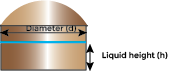
\includegraphics[scale=1]{DigesterWOCDimensions_1}
\end{center}

{
$=\dfrac
	{
		5000
		\dfrac
			{gal \enspace sludge}
			{day}
		*(8.34*0.06*0.66) 
		\dfrac
			{lbs VS}
			{gal \enspace  sludge}
	}
	{
		(\dfrac
			{\pi}
			{4}*37^2*27)ft^3
	}
=\boxed
	{
		0.057 \dfrac
			{lbs \enspace VS}
			{day-ft^3}
	}
$}

\item The sludge feed to a digester is 12,000 $ft^3$/day.  The sludge contains 4.5\% total solids with 70\% volatile solids.  What is the digester loading in lbs VSS/day per $ft^3$ if the digester diameter is 100 ft and a working sludge level of 20 ft.\\
	
Solution:\\
{
$
	Digester \enspace volatile \enspace solids 			\enspace loading \enspace Rate = 					\dfrac
	{
	Digester \enspace loading 
		\dfrac
		{
		lbs \enspace VS
		}
		{
		day
		}
	}
	{
	Digester \enspace volume (V)ft^3
	}
$
}\\

\begin{center}
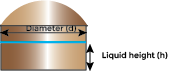
\includegraphics[scale=1]{DigesterWOCDimensions_1}
\end{center}

{
$=\dfrac
	{
		12,000
		\dfrac
			{
			ft^3 \enspace sludge
			}
			{
			day
			}
		*7.48 \dfrac
				{
				gal
				}
				{
				ft^3
				}	
		*(8.34*0.045*0.70) 
		\dfrac
			{lbs VS}
			{gal \enspace  sludge}
	}
	{
		(	\dfrac
			{
			\pi
			}
			{
			4
			}
			*100^2*20
		)
		ft^3
	}
=\boxed
	{
		0.15 \dfrac
			{
			lbs \enspace VS
			}
			{
			day-ft^3
			}
	}
$}\\
\item How much gas is produced in the above digester in $ft^3$/day if the digested sludge contains 2.5\% total solids of which 59\% is volatile solids and the gas production rate is 14 $ft^3$/lb VS destroyed?\\
Solution:\\

{
$
Digester \enspace VS \enspace reduction (\%)=
	\dfrac
	{0.70 - .59}
	{0.70 - 0.70 *0.59}
	*100=38.3\%
$
}\\
\vspace{6mm}

{
$
	\dfrac
	{
	lbs \enspace VS \enspace reduction
	}
	{
	day
	}
	=
	\dfrac
	{
	3153 lbs \enspace VS \enspace feed
		*  0.383 \enspace VS \enspace reduction
	}
	{
	day
	}
 	=1,208
	\dfrac
	{
	lbs \enspace VS \enspace reduction
	}
	{
	day 
	}
$
}\\
\vspace{6mm}

{
$
	\dfrac 
	{
	ft^3 gas \enspace produced
	}
	{
	day
	}
	=
	1208 \dfrac
			{
			lbs \enspace VS \enspace reduced
			}
			{
			day
			}
			*
		\dfrac
		{
		14 ft^3 \enspace gas \enspace produced
		}
		{
		lb \enspace VS \enspace reduced
		}
		=16,912 \dfrac
				{
				ft^3 \enspace digester \enspace 					gas \enspace produced
				}
				{
				day
				}
$
} 
\item The sludge feed to a digester is 80,000 gal/day. The sludge contains 4.5\% total solids with 75\% volatile solids. If 50\% of VS are reduced in the digester: 



\begin{enumerate}
\item Find lbs VS destroyed per 1000 gal of digester capacity per day if the digester radius is 55 ft with an operating sludge level of 25 ft.(5 points)

\vspace{1cm}
Solution:\\
Digester Volume: 
$
{
		(\pi*55^2*25)ft^3 *7.48 \dfrac{gal}{ft^3}
	}=1,776,220 gallons=1,776.2 \enspace(1000 \enspace gallons)
$
\\
\vspace{3mm}
$
	\dfrac
	{
	lbs \enspace VS \enspace reduction
	}
	{
	day
	}
	=
	\dfrac
	{
	80,000 gal * 8.34 \dfrac{lbs}{gal}*(0.045*0.75) \dfrac{lbs VS}{lb}*0.5\dfrac{lbs \enspace VS \enspace  reduction}{lb \enspace VS}
	}
	{
	day
	}$\\
\vspace{0.5cm}
$
 	=11,259
	\dfrac
	{
	lbs \enspace VS \enspace reduction
	}
	{
	day 
	}
$
\\
\vspace{3mm}


$
	\dfrac
	{
	lbs \enspace VS \enspace reduction
	}
	{
	1000 \enspace digester \enspace capacity
	}
	=
	\dfrac
	{
	11,259 \dfrac
			{
			lbs \enspace VS \enspace reduction
			}
			{
			day
			}
	}
	{	
	1,776.2 \enspace (1000 \enspace gallons)
	}
 	=\boxed{6.3
	\dfrac
	{
	lbs \enspace VS \enspace reduction
	}
	{
	1000 gallons \enspace digester \enspace volume 
	}}
$
\\

\vspace{1cm}

\item  What is the digester gas production in Btu/day? Assume 14 cu. ft digester gas per lb of VS destroyed and a 650 Btu/cu. ft heating value for the digester gas produced (5 points)
\end{enumerate}
\vspace{1cm}
Solution:\\

$
	\dfrac 
	{
	ft^3 gas \enspace produced
	}
	{
	day
	}
	=
	11,259 \dfrac
			{
			lbs \enspace VS \enspace reduced
			}
			{
			day
			}
			*
		\dfrac
		{
		14 ft^3 \enspace gas \enspace produced
		}
		{
		lb \enspace VS \enspace reduced
		}
		=157,626 \dfrac
				{
				ft^3 \enspace digester \enspace 					gas \enspace produced
				}
				{
				day
				}
$
\\
\vspace{1cm}


$
	\dfrac 
	{
	BTU \enspace produced
	}
	{
	day
	}
	=
	157,626 \dfrac
			{
			ft^3 \enspace gas \enspace produced
			}
			{
			day
			}
			*
		\dfrac
		{
		650 BTU \enspace gas \enspace produced
		}
		{
		ft^3 gas
		}
		=\boxed{102,456,900 \dfrac
				{
				BTU \enspace produced
				}
				{
				day
				}}
$

\item Two sludges are blended together as follows: 15,000 gal. primary sludge at 4.1\% solids. 28,000 gal. secondary sludge at 1.3\% solids. What is the combined solids concentration?  If the primary sludge is 68\% VS and the secondary sludge is 63\% VS, what is the VS concentration (\%) in the combined sludge?

Solution:

Combined solids concentration:
$
C_1*V_1 + C_2*V_2 = C_3*V_3$\\
$\implies C_3 = \dfrac{C_1*V_1 + C_2*V_2}{V3}=\dfrac{C_1*V_1 + C_2*V_2}{V_1 + V_2}=\dfrac{4.1*15,000 + 1.3*28,000}{15,000 + 28,000}=\boxed{2.28\%}
$\\
Lbs of VS in combined sludge:
$
C\textsubscript{VS1}*V_1 + C\textsubscript{VS2}*V_2 = C\textsubscript{VS3}*V_3$\\
$\implies C\textsubscript{VS3} = \dfrac{C\textsubscript{VS1}*V_1 + C\textsubscript{VS2}*V_2}{V3}=\dfrac{C\textsubscript{VS1}*V_1 + C\textsubscript{VS1}*V_2}{V_1 + V_2}$\\
$\implies C\textsubscript{VS3}
=\dfrac{4.1*15,000*0.68 + 1.3*28,000*0.63}{15,000 + 28,000}=\boxed{1.50\%}$
\\


\item The volatile acids concentration of sludge in an anaerobic digester is 195 mg/l. If the maximum volatile acids:alkalinity ratio is 0.087, what should the alkalinity be in mg/l?\\
Solution:\\
Volatile acid:Alkalinity=0.087=$\dfrac{195}{x}\implies x = \dfrac{195}{0.087} =\boxed{2,241\dfrac{mg}{l}}$
\pagebreak
	
\item 10,000 gallons of sludge is pumped to an anaerobic digester/day at 4\% solids (70\% VS).  50\% of the VS are destroyed, creating 15 $ft^3$ of gas per lbs. of VS destroyed. How much gas is produced each day?\\

{
$
	\dfrac
	{
	lbs \enspace VS \enspace reduction
	}
	{
	day
	}
	=
	\dfrac
	{
	10,000 gal * 8.34 \dfrac{lbs}{gal}*(0.04*0.7) \dfrac{lbs VS}{lb}*\dfrac{0.5 lbs \enspace VS \enspace  reduction}{lb \enspace VS}
	}
	{
	day
	}
 	=1,168
	\dfrac
	{
	lbs \enspace VS \enspace reduction
	}
	{
	day 
	}
$
}\\
\vspace{3mm}

{
$
	\dfrac 
	{
	ft^3 gas \enspace produced
	}
	{
	day
	}
	=
	1,168 \dfrac
			{
			lbs \enspace VS \enspace reduced
			}
			{
			day
			}
			*
		\dfrac
		{
		15 ft^3 \enspace gas \enspace produced
		}
		{
		lb \enspace VS \enspace reduced
		}
		=17,520 \dfrac
				{
				ft^3 \enspace digester \enspace 					gas \enspace produced
				}
				{
				day
				}
$
} 


\item Given a sludge flow of 5,500 gpd with 6.5\% solids containing  72\% VS to a digester with a VS destruction of 48\%   If the digester is digester is 40 ft. diameter with a sludge level of 25 ft, find lbs. VS destroyed per 1000 gal of digester capacity per day.  What is the digester gas production in Btu/day if the \% VS reduction in the digester is 58\% and the digester raw sludge feed is 6000 cu. Ft/day containing 4.5\% total solids with a 64\% VS content?  Assume 13.5 cu. ft digester gas per lb of VS destroyed and a 650 Btu/cu. ft heating value for the digester gas produced\\

{
Digester Volume: 
$
{
		(\dfrac
			{\pi}
			{4}*40^2*25)ft^3 *7.48 \dfrac{gal}{ft^3}
	}=940,086 gallons=940 \enspace(1000 \enspace gallons)
$
}\\
\vspace{3mm}

{
$
	\dfrac
	{
	lbs \enspace VS \enspace reduction
	}
	{
	day
	}
	=
	\dfrac
	{
	5,500 gal * 8.34 \dfrac{lbs}{gal}*(0.065*0.72) \dfrac{lbs VS}{lb}*\dfrac{0.48 lbs \enspace VS \enspace  reduction}{lb \enspace VS}
	}
	{
	day
	}
 	=1,030
	\dfrac
	{
	lbs \enspace VS \enspace reduction
	}
	{
	day 
	}
$
}\\
\vspace{3mm}


{
$
	\dfrac
	{
	lbs \enspace VS \enspace reduction
	}
	{
	1000 \enspace digester \enspace capacity
	}
	=
	\dfrac
	{
	1,030 \dfrac
			{
			lbs \enspace VS \enspace reduction
			}
			{
			day
			}
	}
	{	
	940 \enspace (1000 \enspace gallons)
	}
 	=1.1
	\dfrac
	{
	lbs \enspace VS \enspace reduction
	}
	{
	1000 gallons \enspace digester \enspace volume 
	}
$
}\\
\vspace{3mm}


{
$
	\dfrac 
	{
	ft^3 gas \enspace produced
	}
	{
	day
	}
	=
	1,030 \dfrac
			{
			lbs \enspace VS \enspace reduced
			}
			{
			day
			}
			*
		\dfrac
		{
		13.5 ft^3 \enspace gas \enspace produced
		}
		{
		lb \enspace VS \enspace reduced
		}
		=13,905 \dfrac
				{
				ft^3 \enspace digester \enspace 					gas \enspace produced
				}
				{
				day
				}
$
}\\
\vspace{3mm}



{
$
	\dfrac 
	{
	BTU \enspace produced
	}
	{
	day
	}
	=
	13,905 \dfrac
			{
			ft^3 \enspace gas \enspace produced
			}
			{
			day
			}
			*
		\dfrac
		{
		650 BTU \enspace gas \enspace produced
		}
		{
		ft^3 gas
		}
		=9,038,250 \dfrac
				{
				BTU \enspace produced
				}
				{
				day
				}
$
}

\item Two sludges are blended together as follows: 60,000 gal per day. primary sludge at 4.5\% solids and 28,000 gal secondary sludge at 5\% solids. 
\begin{enumerate}
\item What is the combined solids concentration?  (3 points)\\

$\dfrac{60,000*4.5+28,000*5}{88,000}=\boxed{4.66\%}$\\
\vspace{2cm}
\item How many lbs of solids (per day) are in the combined sludge (3 points)\\

$88,000 gal*8.34*0.0466 = \boxed{34,200 lbs}$\\
\vspace{2cm}


\item If the primary sludge is 68\% VS and the secondary sludge is 83\% VS, how many pounds of VS are in the combined sludge? (3 points)\\
$60,000 gal *\dfrac{8.34*0.045*0.68lbs \enspace VS}{gal}+28,000 gal *\dfrac{8.34*0.05*0.83lbs \enspace VS}{gal}=\boxed{25,003 lbs \enspace VS}$
\vspace{2cm}

\item What is the digester feed VS\%?  (3 points)\\
$\dfrac{25,003 lbs \enspace VS}{34,200 lbs TS}=\boxed{73.1\%}$

\vspace{2cm}



\item If the digester is 120’ diameter with a liquid height of 20’, what is the VS loading in lbs VS/ft3-day (3 points)\\

$\dfrac{25,003 lbs \enspace VS}{0.785*120^2*20}=\boxed{\dfrac{0.11 lbs \enspace VS}{day-ft^3}}$\\
\vspace{2cm}





\item If the digested sludge has 52\% VS, calculate the digester VS reduction percent (3 points)\\

$
Digester \enspace VS \enspace reduction (\%)=
	\dfrac
	{0.731 - .52}
	{0.731 - 0.731 *0.52}
	*100=\boxed{60.1\%}
$\\
\vspace{2cm}

\item What is the gas production (ft$^3$/day) if the digester produces 14 ft$^3$ gas/lb VS destroyed (3 points)\\
25,003*0.601$\dfrac{lbs\enspace VS destroyed}{}*\dfrac{14ft^3 \enspace gas \enspace produced}{lb \enspace VS \enspace destroyed}=\boxed{210,375ft^3 gas}$
\\
\vspace{2cm}

\item How many belt presses are needed to keep up with the digested sludge flow if the belt presses can be operated at a maximum flow of 50 GPM (3 points)\\

88,000$\dfrac{gal \enspace sludge}{day}*\dfrac{day}{1440min}=61 GPM$\\
@50 GPM per press - $\boxed{2 \enspace BFP \enspace required}$
\vspace{2cm}
\item If the digested sludge feed to the belt filter presses is 2.6\% and assuming the belt press feed solids capture is 90\%.  How many lbs of solids (dry) are produced by the BFP (4 points)\\
$88,000\dfrac{gal}{day}*8.34*0.026\dfrac{lbs \enspace solids \enspace feed}{day}*0.9\dfrac{lbs \enspace solids \enspace captured}{lbs \enspace solids \enspace feed}=\boxed{17,174 lbs \enspace solids \enspace per \enspace day}$
\vspace{2cm}

\item If the BFP produces a 20\% cake, how many wet tons cake produced per day (4 points)\\
$\dfrac{17,174 lbs \enspace solids \enspace produced}{day}*\dfrac{100 lbs \enspace cake}{20 lbs \enspace solids \enspace produced}*\dfrac{tons}{2,000 lbs}=\boxed{\dfrac{42.9tons}{day}}$
\vspace{2cm}

\item If the cake density is 68 lbs/cu. ft, how much time will it take to fill a 30 cu. yd bin (3 points)\\
(Ans. 15.4 hours)
$\dfrac{(42.9*2000)lbs \enspace cake}{day}*\dfrac{day}{1440 min}=\dfrac{59.583}{lbs \enspace cake}{min}$\\
$\dfrac{59.583}{lbs \enspace cake}{min}*\dfrac{ft^3}{68 lbs \enspace cake}=\dfrac{0.876ft^3}{min}$\\
$30yd^3*\dfrac{27ft^3}{yd^3}*\dfrac{min}{0.876ft^3}*\dfrac{hrs}{60 min}=\boxed{15.4hrs}$
\vspace{2cm}
\item What will be the cost of hauling dewatered cake per day @ \$65 per ton cake (2 points)\\
42.9$\dfrac{tons}{day}*\dfrac{\$65}{ton}=\boxed{\dfrac{\$2,789}{day}}$ 
\end{enumerate}

\item Calculate the VS loading to the digester in lbs/day if 10,000 cu. ft of sludge containing 4.8\% TS with and an average VS content of 82\% 




\item Calculate the VS loading to the digester in lbs/day if 25,000 gallons of sludge containing 4.5\% TS with and average VS content of 76\% is fed to the digester 

Solution:\\
$\dfrac{25,000 \enspace Gal}{day}*\dfrac{8.34 \enspace lbs \enspace sludge}{Gal}* \dfrac{(0.045*0.76) \enspace lbs \enspace VS \enspace feed}{lb \enspace sludge}=\boxed{\dfrac{7,131 \enspace lbs \enspace VS }{day} } $


\item Calculate the \% VS reduction in a digester given the volatile solids content of the feed sludge to the digester is 76\% and the volatile solids content of the sludge leaving the digester is 55\% 




\item Calculate the organic loading rate to two 320,000 gallon anaerobic digesters given:
Primary sludge feed rate of 25,000 gallons with 6.2\% TS containing 73\% solids and SG of 1.03.
Secondary sludge feed rate of 30,500 gallons with 3.8\% TS containing 77\% solids (7 points)
(Answer: 0.2lbs VS/day-ft3 ) 

\item 10,000 gallons/day of sludge is pumped to an anaerobic digester/day at 4\% solids (70\% VS).  If 50\% of the VS is destroyed, how many lbs of VS is destroyed per day?\\
Solution:\\
$\dfrac{10,000 \enspace Gal}{day}*\dfrac{8.34 \enspace lbs \enspace sludge}{Gal} \dfrac{0.04*0.7 \enspace lbs \enspace VS \enspace feed}{lb \enspace sludge}*\dfrac{0.5 \enspace lbs \enspace VS \enspace destroyed}{lbs \enspace VS \enspace feed}=\boxed{\dfrac{1,168lbs \enspace VS \enspace destroyed}{day} } $

\item A DAF thickener has effluent solids of 55 mg/L and float solids of 2.0\%. Solids loading and polymer dosing is in the normal range. This data likely indicates: \\

a. This unit is operating normally \\
b. Too low air to solids ratio \\
c. Float blanket too thick \\
*d. Flight speed too fast \\
e. Flight speed too slow \\

\item  An air flotation thickener will produce a thin float if: \\

*a. Flight speed too high and skimmer wiper not adjusted properly \\
b. Excessive air/solids ratio and polymer dosages too low \\
c. High dissolved oxygen and flight speed too low \\
d. Polymer dosages too high and unit overloaded \\

\item  An increase in the pool depth of a scroll-type centrifuge: \\

a. would not affect the moisture content of the cake. \\
b. would produce a drier cake \\
*c. would produce a wetter cake, but produce a greater solids recovery. \\
d. would not affect either solids recovery, nor cake moisture content. \\
e. would require an increase in the cationic polymer dosage. \\

\item  A sludge thickened from 1\% to 4\% solids will be reduced in volume by how much? \\

a. no more than 4\% of original volume \\
b. approximately 17\% of original volume \\
*c. approximately 25\% of original volume* \\
d. more information is needed \\

\item  Gravity thickeners, compared to DAFs, are best suited to: \\

*a. Thickening primary sludge. \\
b. Thickening waste activated sludge. \\
c. Controlling sulfide odors. \\
d. Removing filamentous bacteria. \\
e. Provide highest concentration sludge. \\

\item  Gravity thickeners, compared to DAFTs, are best suited to: \\

*a. Thickening primary sludge \\
b. Thickening waste activated sludge \\
c. Controlling sulfide odors \\
d. Removing filamentous bacteria \\
e. Provide highest concentration sludge \\

\item  Identify the incorrect statement regarding gravity thickeners. \\

a. Gravity thickeners are similar in design to primary clarifiers. \\
*b. The sludge blanket depth and the rate of sludge withdrawal are used to calculate the sludge detention time. \\
c. The purpose of pickets in a sludge thickener is to gently stir settling sludge particles to release gases that may prevent the sludge particles from compacting. \\
d. Mixtures of primary and waste activated sludge are never thickened in a gravity thickener due to the possibilility of de-nitrification. \\
e. Solids loading (pounds per day per square foot) is an important guideline for a gravity thickener. \\

\item  On a routine check of a DAF unit the operator finds suspended solids of 450 mg/L in the effluent. The float blanket appears well flocculated and concentrated. The operator should: \\

*a. Increase the flight speed. \\
b. Do nothing, the unit is operating normally. \\
c. Reduce the air to solids ratio. \\
d. Increase the air to solids ratio. \\
e. Check unit operating pressure. \\

\item  On a routine check of a DAFT unit the operator finds suspended solids of 450 mg/L in the effluent.  The float blanket appears well flocculated and concentrated. The operator should: \\

a. increase the flight speed \\
b. do nothing, the unit is operating normally \\
c. reduce the air to solids ratio \\
*d. increase the air to solids ratio \\
e. check unit operating pressure \\

\item  Which of the following is not the main reason for thickening sludge \\

a. Improved digester performance due to a lower volume of sludge \\
b. Cost savings in the construction of new digestion facilities \\
c. Reduction in anaerobic digestion heating requirements since less water has to be heated \\
*d. Reduce costs of biosolids hauling \\

\item  What zone is not involved in a belt filter press? \\

a. Gravity \\
b. Low pressure (wedge) \\
c. High pressure \\
*d. Twilight \\

\item  The float blanket in a DAF unit appears well flocculated and concentrated.  Too low a flight speed would likely result in: \\

a. Using excessive amounts of air. \\
b. Float solids that are too thick. \\
c. Too low an air-to-solids ratio. \\
*d. Poor thickener underflow quality. \\
e. De-flocculation of float solids. \\

\item  The least critical operational control of a dissolved air flotation thickener in producing an adequately thickened sludge is the: \\

a. Flight speed. \\
b. Air to solids ratio. \\
c. Polymer dosage. \\
*d. Recycle ratio. \\
e. Pre-thickened WAS concentration. \\

\item  The operational control of a dissolved air flotation thickener most critical for producing an adequately thickened float solids is the: \\

a. Fight speed. \\
*b. Air to solids ratio. \\
c. Polymer dosage. \\
d. Recycle ratio. \\
e. Concentration of WAS being thickened. \\

\item  To increase solids recovery on a dual belt, belt press, the operator should: \\

a. Increase the differential belt speed. \\
b. Increase belt speed. \\
c. Increase sludge feed rate. \\
*d. Decrease sludge feed rate. \\
e. Increase polymer feed. \\

\item  Too high a flight speed in a DAF will likely result in: \\

a. Using excessive amounts of air. \\
b. Excessive underflow volume. \\
*c. Thin float solids. \\
d. Too high an air to solids ratio. \\
e. Too low an air to solids ratio. \\

\item  What can be a problem with a belt filter press? \\

a. Washing out \\
b. Polymer overdosing \\
c. Blinding \\
*d. All of the above \\

\item  What can be used to evaluate the efficiency of a belt filter press? \\

a. Vacuum required in inches of mercury \\
b. \% volatile solids in cake \\
c. Sludge feed rate in gpd \\
*d. Filter yield in lbs/hr/sq ft \\
e. Gph of filtrate removal. \\

\item  Which of the following is not the main reason for thickening sludge \\

a. Improved digester performance due to a lower volume of sludge \\
b. Cost savings in the construction of new digestion facilities \\
c. Reduction in anaerobic digestion heating requirements since less water has to be heated \\
*d. Reduce costs of biosolids hauling \\

\item  Which one of the following statements is TRUE in regard to DAF thickeners? \\

*a. The air to solids ratio in a DAF unit is typically 0.03 to 0.05. \\
b. The speed of the so-called "flights" has very little effect on the concentration of the float solids. \\
c. Adjustments in the air to solids ratio in a DAF unit will affect the float solids but not the unit's effluent suspended solids. \\
d. Anionic polymers are typically used to condition the WAS feed to a DAF unit. \\

\item  Which one of the following process units is usually classified as a sludge thickening device as opposed to a dewatering device: \\

*a. DAF unit. \\
b. Sludge drying bed. \\
c. Vacuum filter press. \\
d. Belt press. \\
e. All of the above are thickeners, not dewatering devices. \\

\item  Which one the following statements is TRUE in regard to gravity thickeners? \\

a. Longer solids detention times are desired during summer operation of these units. \\
b. The sludge-volume-ratio (SVR) or sludge detention time is defined as the volume of the sludge blanket divided by the daily volume of sludge withdrawn from the thickener. \\
c. SVRs should be in range of 5 to 10 hours. \\
*d. A likely cause of a gravity thickener producing a poor quality effluent is too low of a sludge blanket.* \\

\item  In a gravity thickener the depth of the sludge is kept minimal (<six inches) to avoid solids going over the effluent weir \\

a. True \\
*b. False \\

\item  Sludge thickening is primarily conducted to reduce costs associated with biosolids hauling\\


a. True \\
*b. False \\

\item  Sludge thickening is primarily conducted to reduce costs associated with biosolids hauling \\

a. True \\
*b. False \\

\item  Gravity thickener is commonly used for sludge dewatering \\

a. True \\
*b. False \\

\item  Sludge thickening is primarily conducted to reduce costs associated with biosolids hauling \\

a. True \\
*b. False \\

\item  Which one of the following statements is TRUE in regard to the operation of a belt filter press: \\

a. Unlike a gravity belt, cationic polymers need not be used to condition the feed sludge to this unit. \\
b. When dewatering a mixture of WAS and primary sludge, which has been anaerobically digested, the operator can expect to produce a sludge cake with 22\% TS to 25\%. \\
*c. The best belt speed for this unit is the slowest speed the belt can be operated at, without causing “washout.” \\
d. Colloidal solids are likely to cause plugging of belt pores and thus cause “belt binding.” \\

\item  In your own words, what does sludge stabilization accomplish. (4 points)\\
What are the different methods utilized for sludge stabilization (4 points)\\

Correct Answer(s): \\

\item  Explain the benefits of sludge thickening \\

Correct Answer(s): \\

\item  Define sludge volume ratio and what is the significance of this term in gravity thickening \\

Correct Answer(s): \\

\item  in your opinion what are the key operational parameters of the DAFT and why are they key \\

Correct Answer(s): \\

\item  What is the key difference between sludge thickening and sludge dewatering \\

Correct Answer(s): \\

\item  In your own words, what does sludge stabilization accomplish. (4 points)\\
What are the different methods utilized for sludge stabilization (4 points)\\

Correct Answer(s): \\

\item  Why is solids stabilization critical \\

Correct Answer(s): \\

\item  List four reasons for treating wastewater solids \\

Correct Answer(s): \\

\item  Explain the significance of pond depth in centrifuge operation \\

Correct Answer(s): \\

\item  Explain the benefits of sludge thickening \\

Correct Answer(s): \\

\item  Define sludge volume ratio and what is the significance of this term in gravity thickening \\

Correct Answer(s): \\

\item  in your opinion what are the key operational parameters of the DAFT and why are they key \\

Correct Answer(s): \\

\item  What is the key difference between sludge thickening and sludge dewatering \\

Correct Answer(s): \\

\item  In your own words, what does sludge stabilization accomplish. (4 points)\\
What are the different methods utilized for sludge stabilization (4 points)\\

Correct Answer(s): \\

\item  Why is solids stabilization critical \\

Correct Answer(s): \\

\item  List four reasons for treating wastewater solids \\

Correct Answer(s): \\

\item  Explain the significance of pond depth in centrifuge operation \\

Correct Answer(s): \\

\item  325 GPM of WAS with 7,000 mg/l TSS is thickened in a DAFT. Assuming an air:solids ratio of 0.05 lb of air for each lb of feed solids, The SCFM (standard cubic feed per minute) air required to thicken the WAS given 1 SCFM = 0.075 lb is: \\

*a. 12.6 SCFM \\
b. 0.126 SCFM \\
c. 12,600 SCFM \\
d. 1.26 SCFM \\

\item  325 GPM of WAS with 7,000 mg/l TSS is thickened in a DAFT. Assuming an air:solids ratio of 0.05 lb of air for each lb of feed solids, The SCFM (standard cubic feed per minute) air required to thicken the WAS given 1 SCFM = 0.075 lb is: \\

*a. 12.6 SCFM \\
b. 0.126 SCFM \\
c. 12,600 SCFM \\
d. 1.26 SCFM \\

\item  When you spread sludge on agricultural land, the annual application rate of cadmium in the sludge should be less than 2 lbs/acre/year If your sludge contains 30 mg cadmium per kilogram of solids and your plant produces 950,000 lbs per year of dry solids, how many acres do you need? \\

a. 3 acres \\
*b. 14 acres \\
c. 19 acres \\
d. 27 acres \\

\item  A DAF thickener has effluent solids of 55 mg/L and float solids of 2.0\%. Solids loading and polymer dosing is in the normal range. This data likely indicates: \\

a. This unit is operating normally \\
b. Too low air to solids ratio \\
c. Float blanket too thick \\
*d. Flight speed too fast \\
e. Flight speed too slow \\

\item  An air flotation thickener will produce a thin float if: \\

*a. Flight speed too high and skimmer wiper not adjusted properly \\
b. Excessive air/solids ratio and polymer dosages too low \\
c. High dissolved oxygen and flight speed too low \\
d. Polymer dosages too high and unit overloaded \\

\item  An increase in the pool depth of a scroll-type centrifuge: \\

a. would not affect the moisture content of the cake. \\
b. would produce a drier cake \\
*c. would produce a wetter cake, but produce a greater solids recovery. \\
d. would not affect either solids recovery, nor cake moisture content. \\
e. would require an increase in the cationic polymer dosage. \\

\item  A sludge thickened from 1\% to 4\% solids will be reduced in volume by how much? \\

a. no more than 4\% of original volume \\
b. approximately 17\% of original volume \\
*c. approximately 25\% of original volume* \\
d. more information is needed \\

\item  Gravity thickeners, compared to DAFs, are best suited to: \\

*a. Thickening primary sludge. \\
b. Thickening waste activated sludge. \\
c. Controlling sulfide odors. \\
d. Removing filamentous bacteria. \\
e. Provide highest concentration sludge. \\

\item  Gravity thickeners, compared to DAFTs, are best suited to: \\

*a. Thickening primary sludge \\
b. Thickening waste activated sludge \\
c. Controlling sulfide odors \\
d. Removing filamentous bacteria \\
e. Provide highest concentration sludge \\

\item  Identify the incorrect statement regarding gravity thickeners. \\

a. Gravity thickeners are similar in design to primary clarifiers. \\
*b. The sludge blanket depth and the rate of sludge withdrawal are used to calculate the sludge detention time. \\
c. The purpose of pickets in a sludge thickener is to gently stir settling sludge particles to release gases that may prevent the sludge particles from compacting. \\
d. Mixtures of primary and waste activated sludge are never thickened in a gravity thickener due to the possibilility of de-nitrification. \\
e. Solids loading (pounds per day per square foot) is an important guideline for a gravity thickener. \\

\item  On a routine check of a DAFT unit the operator finds suspended solids of 450 mg/L in the effluent.  The float blanket appears well flocculated and concentrated. The operator should: \\

a. increase the flight speed \\
b. do nothing, the unit is operating normally \\
c. reduce the air to solids ratio \\
*d. increase the air to solids ratio \\
e. check unit operating pressure \\

\item  Which of the following is not the main reason for thickening sludge \\

a. Improved digester performance due to a lower volume of sludge \\
b. Cost savings in the construction of new digestion facilities \\
c. Reduction in anaerobic digestion heating requirements since less water has to be heated \\
*d. Reduce costs of biosolids hauling \\

\item  What zone is not involved in a belt filter press? \\

a. Gravity \\
b. Low pressure (wedge) \\
c. High pressure \\
*d. Twilight \\

\item  Lowering the vat depth of a vacuum filter is most likely to produce \rule{1.5cm}{0.3mm} cake produce \\

a. Wetter \\
b. Thicker \\
c. Stronger \\
*d. Dryer \\

\item  You have observed water spraying out of the vacuum filter's silencer (or snubber; exhaust pipe Which of the following conditions is the most likely cause of the problem? \\

a. Filtrate pump not functioning properly \\
*b. Vacuum too high \\
c. Vacuum too low \\
d. Worn check valves in vacuum system \\

\item  An air flotation thickener will produce a thin float if \\

a. Flight speed too high and skimmer wiper not adjusted properly \\
*b. Excessive air/solids ratio and polymer dosages too low \\
c. High dissolved oxygen and flight speed too low \\
d. Polymer dosages too high and unit overloaded. \\

\item  Gravity-thickened primary sludge will contain solids within which of the following concentration ranges? \\

a. 1,000 - 8,000 mg/l \\
b. 10,000 – 40,000 mg/l \\
c. 40,000 - 80,000 mg/l \\
d. 100,000 - 400,000 mg/l \\
*e. none of the above \\

\item  The float blanket in a DAF unit appears well flocculated and concentrated.  Too low a flight speed would likely result in: \\

a. Using excessive amounts of air. \\
b. Float solids that are too thick. \\
c. Too low an air-to-solids ratio. \\
*d. Poor thickener underflow quality. \\
e. De-flocculation of float solids. \\

\item  The least critical operational control of a dissolved air flotation thickener in producing an adequately thickened sludge is the: \\

a. Flight speed. \\
b. Air to solids ratio. \\
c. Polymer dosage. \\
*d. Recycle ratio. \\
e. Pre-thickened WAS concentration. \\

\item  The operational control of a dissolved air flotation thickener most critical for producing an adequately thickened float solids is the: \\

a. Fight speed. \\
*b. Air to solids ratio. \\
c. Polymer dosage. \\
d. Recycle ratio. \\
e. Concentration of WAS being thickened. \\

\item  To increase solids recovery on a dual belt, belt press, the operator should: \\

a. Increase the differential belt speed. \\
b. Increase belt speed. \\
c. Increase sludge feed rate. \\
*d. Decrease sludge feed rate. \\
e. Increase polymer feed. \\

\item  What can be a problem with a belt filter press? \\

a. Washing out \\
b. Polymer overdosing \\
c. Blinding \\
*d. All of the above \\

\item  What can be used to evaluate the efficiency of a belt filter press? \\

a. Vacuum required in inches of mercury \\
b. \% volatile solids in cake \\
c. Sludge feed rate in gpd \\
*d. Filter yield in lbs/hr/sq ft \\
e. Gph of filtrate removal. \\

\item  Which of the following is not the main reason for thickening sludge \\

a. Improved digester performance due to a lower volume of sludge \\
b. Cost savings in the construction of new digestion facilities \\
c. Reduction in anaerobic digestion heating requirements since less water has to be heated \\
*d. Reduce costs of biosolids hauling \\

\item  Which one of the following process units is usually classified as a sludge thickening device as opposed to a dewatering device: \\

*a. DAF unit. \\
b. Sludge drying bed. \\
c. Vacuum filter press. \\
d. Belt press. \\
e. All of the above are thickeners, not dewatering devices. \\

\item  Which one of the following statements is TRUE in regard to DAF thickeners? \\

*a. The air to solids ratio in a DAF unit is typically 0.03 to 0.05. \\
b. The speed of the so-called "flights" has very little effect on the concentration of the float solids. \\
c. Adjustments in the air to solids ratio in a DAF unit will affect the float solids but not the unit's effluent suspended solids. \\
d. Anionic polymers are typically used to condition the WAS feed to a DAF unit. \\

\item  Which one of the following process units is usually classified as a sludge thickening device as opposed to a dewatering device: \\

*a. DAF unit. \\
b. Sludge drying bed. \\
c. Vacuum filter press. \\
d. Belt press. \\
e. All of the above are thickeners, not dewatering devices. \\

\item  Which one of the following statements is TRUE in regard to the operation of a belt filter press: \\

a. Unlike a gravity belt, cationic polymers need not be used to condition the feed sludge to this unit. \\
b. When dewatering a mixture of WAS and primary sludge, which has been anaerobically digested, the operator can expect to produce a sludge cake with 22\% TS to 25\%. \\
*c. The best belt speed for this unit is the slowest speed the belt can be operated at, without causing “washout.” \\
d. Colloidal solids are likely to cause plugging of belt pores and thus cause “belt binding.” \\

\item  Which one the following statements is TRUE in regard to gravity thickeners? \\

a. Longer solids detention times are desired during summer operation of these units. \\
b. The sludge-volume-ratio (SVR) or sludge detention time is defined as the volume of the sludge blanket divided by the daily volume of sludge withdrawn from the thickener. \\
c. SVRs should be in range of 5 to 10 hours. \\
*d. A likely cause of a gravity thickener producing a poor quality effluent is too low of a sludge blanket.* \\

\item  Match the sludge treatment methods \\

\item  In a gravity thickener the depth of the sludge is kept minimal (<six inches) to avoid solids going over the effluent weir \\

a. True \\
*b. False \\

\item  In a decanter centrifuge, greater pond depth would produce drier cake \\

a. True \\
*b. False \\

\item  Sludge thickening is primarily conducted to reduce costs associated with biosolids hauling\\

a. True \\
*b. False \\

\item  Sludge thickening is primarily conducted to reduce costs associated with biosolids hauling \\

a. True \\
*b. False \\

\item  Gravity thickener is commonly used for sludge dewatering \\

a. True \\
*b. False \\

\item  Grit and screenings from the preliminary treatment are also considered as biosolids \\

*a. True \\
b. False \\

\item  In a decanter centrifuge, greater pond depth would produce drier cake \\

a. True \\
*b. False \\

\item  Sludge thickening is primarily conducted to reduce costs associated with biosolids hauling \\

a. True \\
*b. False \\

\item  Two sludges are blended together as follows: 8,000 cu. ft primary sludge at 4.90\% solids and 23,000 gal. secondary sludge at 5.20\% solids. What is the combined solids concentration?\\


a. 3.84 \\
b. 6.23 \\
c. 5.12 \\
*d. 4.98 \\

\item  Two sludges are blended together as follows: 8,000 cu. ft primary sludge at 4.90\% solids and 23,000 gal. secondary sludge at 5.20\% solids. What is the combined solids concentration?\\


a. 3.84 \\
b. 6.23 \\
c. 5.12 \\
*d. 4.98 \\

\item  Which one of the following statements is TRUE in regard to the operation of a belt filter press: \\

a. Unlike a gravity belt, cationic polymers need not be used to condition the feed sludge to this unit. \\
b. When dewatering a mixture of WAS and primary sludge, which has been anaerobically digested, the operator can expect to produce a sludge cake with 22\% TS to 25\%. \\
*c. The best belt speed for this unit is the slowest speed the belt can be operated at, without causing “washout.” \\
d. Colloidal solids are likely to cause plugging of belt pores and thus cause “belt binding.” \\

\item  A primary clarifier receives an average flow of 12 MGD containing 280mg/L of TSS.  The typical primary removal efficiency is 75\% and produces a 3.5\% sludge and the sludge pump is rated to pump 70 cu.ft/min.\\
1.  How many pounds of TSS is removed in the clarifier?  5 points\\
2. How many cu.ft of sludge at the given 3.5\% sludge needs to be pumped per day to remove the solids?  5 points\\
3. How many minutes would the sludge pump need to be operational each day to pump the required amount of sludge (calculated from 2 above)? 3 points\\
4.  For how many minutes each hour the sludge pump should be programmed to operate (Given the number of minutes the pump need to operate per day calculated from 3 above) ?  2 points  \\

Correct Answer(s): \\

\item  Given the following information, how many gallons of primary sludge containing 5 \% solids must be pumped daily?\\
Flow:  3 mgd\\
Primary influent TSS:  200 mg/l\\
Primary effluent TSS: 100mg/l\\

Correct Answer(s):
a. 6000.0
b. 0.0
c. 0.0
d. 0.0 \\

\item  A sludge pump is set to pump 5 minutes each hour.  It pumps at the rate of 35 gpm.  How many cubic feet of sludge is pumped each day? \\

Correct Answer(s):
a. 561.0
b. 0.0
c. 0.0
d. 0.0 \\

\item  How long will it take (hrs) to fill a 2 ac-ft pond if the pumping rate is 400 GPM \\

Correct Answer(s):
a. 27.0
b. 0.0
c. 0.0
d. 0.0 \\

\item  Given the tank is 10ft wide, 12 ft long and 18 ft deep tank including 2 ft of freeboard when filled to capacity.  How much time (minutes) will be required to pump down this tank to a depth of 2 ft when the tank is at maximum capacity using a 600 GPM pump  \\

Correct Answer(s):
a. 21.0
b. 0.0
c. 0.0
d. 0.0 \\

\item  A sludge pump is set to pump 5 minutes each hour. It pumps at the rate of 35 gpm. How many gallons of sludge are pumped each day? \\

a. 120 gpd \\
b. 175 gpd \\
c. 840 gpd \\
*d. 4200 gpd \\

\item  Calculate the waste sludge pumping rate if you want to waste 2,000 pounds per day of solids with a concentration of return sludge at 5000 mg/L. \\

a. 29 gpm. \\
*b. 33 gpm. \\
c. 35 gpm. \\
d. 37 gpm. \\

\item  How many pounds og solids are pumped to a digester each day if the digester receives 10,000 gpd of sludge at 5\% density \\

a. 417 lbs/day \\
b. 1,479 lbs/day \\
c. 2,337 lbs/day \\
d. 3,273 lbs/day \\
*e. 4,170 lbs/day \\

\item  How many pounds og solids are pumped to a digester each day if the digester receives 10,000 gpd of sludge at 5\% density \\

a. 417 lbs/day \\
b. 1,479 lbs/day \\
c. 2,337 lbs/day \\
d. 3,273 lbs/day \\
*e. 4,170 lbs/day \\

\item  Primary sludge containing five (5\%) solids is pumped to a digester continuously at a rate of 25 gpm.  How many pounds of volatile solids are added to the digester each day if the volatile solids content is 73\% of the total solids \\

a. 1,310 lbs/day \\
b. 1,800 lbs/day \\
c. 9,830 lbs/day \\
*d. 10,960 lbs/day \\
e. 15,010 lbs/day \\

\item  In a 2.1 MGD wastewater treatment plant the influent suspended solids concentration to the primary clarifier is 240 mg/l.  The primary sludge contains 3.2\% TSS and the primary effluent has a suspended solids concentration of 125mg/l.  How many gallons sludge should be pumped per day? \\

a. 63,000 gal/day \\
b. 32,000 gal/day \\
c. 8,200 gal/day \\
*d. 7,550 gal/day \\

\item  A sludge pump is set to pump 5 minutes each hour. It pumps at the rate of 35 gpm. How many gallons of sludge are pumped each day\\

\item  a. 120 gpd \\
b. 175 gpd \\
c. 840 gpd \\
*d. 4200 gpd \\

\item  A sludge pump is set to pump 5 minutes each hour. It pumps at the rate of 35 gpm. How many gallons of sludge are pumped each day? \\

a. 120 gpd \\
b. 175 gpd \\
c. 840 gpd \\
*d. 4200 gpd \\

\item  Which one of the following process units is usually classified as a sludge thickening device as opposed to a dewatering device: \\

*a. DAF unit. \\
b. Sludge drying bed. \\
c. Vacuum filter press. \\
d. Belt press. \\
e. All of the above are thickeners, not dewatering devices. \\

\item  Calculate the VS loading to the digester in lbs/day if 10,000 cu. ft of sludge containing 4.8\% TS with and an average VS content of 82\%\\

Correct Answer(s):
a. 24554.0
b. 0.0
c. 0.0
d. 0.0 \\

\item  Calculate the VS loading to the digester in lbs/day if 25,000 gallons of sludge containing 4.5\% TS with and average VS content of 76\% is fed to the digester\\

Correct Answer(s):
a. 7131.0
b. 0.0
c. 0.0
d. 0.0 \\

\item  Calculate the \% VS reduction in a digester given the volatile solids content of the feed sludge to the digester is 76\% and the volatile solids content of the sludge leaving the digester is 55\%\\

Correct Answer(s):
a. 61.4
b. 0.0
c. 0.0
d. 0.0 \\

\item  If an anaerobic digester receives sludge with VS of 76\% and discharges digested sludge with a 56\% VS.  Its VS reduction is:\\

a. 36\% \\
b. 48\% \\
*c. 60\% \\
d. 89\% \\

\item  If an anaerobic digester receives sludge with VS of 80\% and discharges digested sludge with a 60\% VS.  Its VS reduction is:\\

a. 20\% \\
b. 25\% \\
*c. 63\% \\
d. 89\% \\

\item  Calculate the volatile solids reduction in an anaerobic digester given the following information:  Raw sludge feed to digester:  73.7 \% VS and digested sludge: 57.2 \%VS\\

*a. 52.3\% \\
b. 64 \\
c. 16.5\% \\
d. 42\% \\

\item  If an anaerobic digester receives sludge with VS of 80\% and discharges digested sludge with a 60\% VS.  Its VS reduction is:\\

a. 20\% \\
b. 25\% \\
*c. 63\% \\
d. 89\% \\

\item  If an anaerobic digester receives sludge with VS of 80\% and discharges digested sludge with a 60\% VS.  Its VS reduction is:\\

a. 20\% \\
b. 25\% \\
*c. 63\% \\
d. 89\% \\

\item  If an anaerobic digester receives sludge with VS of 80\% and discharges digested sludge with a 60\% VS.  Its VS reduction is:\\

a. 20\% \\
b. 25\% \\
*c. 63\% \\
d. 89\% \\

\item  Volatile solids removal efficiency of a digester is most commonly monitored utilizing the BOD test\\

a. True \\
*b. False \\

\item  In an anaerobic digester, the [1] is destroyed producing [2].  The digester gas production is typically in the range of [3] cubic feet of digester gas per lb of volatile matter destroyed. \\

\item  In an anaerobic digester, the [1] is destroyed producing [2].  The digester gas production is typically in the range of [3] cubic feet of digester gas per lb of volatile matter destroyed. \\

\item  Calculate the VS loading to the digester in lbs/day if 10,000 cu. ft of sludge containing 4.8\% TS with and an average VS content of 82\% \\

Correct Answer(s):
a. 24554.0 \\

\item  Calculate the VS loading to the digester in lbs/day if 25,000 gallons of sludge containing 4.5\% TS with and average VS content of 76\% is fed to the digester \\

Correct Answer(s):
a. 7131.0 \\

\item  Calculate the \% VS reduction in a digester given the volatile solids content of the feed sludge to the digester is 76\% and the volatile solids content of the sludge leaving the digester is 55\% \\

Correct Answer(s):
a. 61.4 \\

\item  Calculate the organic loading rate to two 320,000 gallon anaerobic digesters given:
Primary sludge feed rate of 25,000 gallons with 6.2\% TS containing 73\% solids and SG of 1.03.
Secondary sludge feed rate of 30,500 gallons with 3.8\% TS containing 77\% solids (7 points)
(Answer: 0.2lbs VS/day-ft3 ) \\

Correct Answer(s): \\

\item  If an anaerobic digester receives sludge with VS of 76\% and discharges digested sludge with a 56\% VS.  Its VS reduction is: \\

a. 36\% \\
b. 48\% \\
*c. 60\% \\
d. 89\% \\

\item  Calculate the volatile solids reduction in an anaerobic digester given the following information:  Raw sludge feed to digester:  73.7 \% VS and digested sludge: 57.2 \%VS \\

*a. 52.3\% \\
b. 64 \\
c. 16.5\% \\
d. 42\% \\

\item  If an anaerobic digester receives sludge with VS of 80\% and discharges digested sludge with a 60\% VS.  Its VS reduction is: \\

a. 20\% \\
b. 25\% \\
*c. 63\% \\
d. 89\% \\

\item  Calculate the VS loading to the digester in lbs/day if 10,000 cu. ft of sludge containing 4.8\% TS with and an average VS content of 82\% \\

a. 42,756 lbs/day \\
*b. 24,554 lbs/day \\
c. 30,987 lbs/day \\
d. 3,256 lbs/day \\

\item  Calculate the VS loading to the digester in lbs/day if 25,000 gallons of sludge containing 4.5\% TS with and average VS content of 76\% is fed to the digester \\

*a. 7,131 lbs/day \\
b. 17,432 lbs/day \\
c. 19,256 lbs/day \\
d. 26,244 lbs/day \\

\item  Calculate the \% VS reduction in a digester given the volatile solids content of the feed sludge to the digester is 76\% and the volatile solids content of the sludge leaving the digester is 55\% \\

a. 56\% \\
b. 38\% \\
c. 42\% \\
*d. 61.4\% \\

\item  What is the digester efficiency if the volatile solids concentration entering an anaerobic digester is 70\% and the volatile solids concentration leaving the digester is 50\%? \\

*a. 29\% \\
b. 40\% \\
c. 57\% \\
d. 71\% \\

\item  You are operating a 1 MGD trickling filter plant with a single stage anaerobic digester You pump about 3,000 gpd of sludge to the fixed cover digester.  The supernatant has a BOD of 950 mg/L The BOD loading coming from the supernatant in pounds per day is \\

a. 12 \\
*b. 24 \\
c. 36 \\
d. 48 \\

\item  How many pounds of solids are pumped to a digester each day, if the digester receives 10,000 gpd of sludge at 5\% density? \\

a. 417 lbs/day \\
b. 1,497 lbs/day \\
c. 2,337 lbs/day \\
d. 3,273 lbs/day \\
*e. 4,170 lbs/day \\

\item  Primary sludge containing five percent (5\%) solids is pumped to a digester continuously at a rate of 25 gpm. How many pounds of volatile solids are added to the digester each day if the volatile solids content is 73\% of the total solids? \\

a. 1,310 lbs/day \\
b. 1,800 lbs/day \\
c. 9,830 lbs/day \\
*d. 10,960 lbs/day \\
e. 15,010 lbs/day \\

\item  Calculate the volatile solids reduction in an anaerobic digester given the following information:  Raw sludge feed to digester:  73.7 \% VS and digested sludge: 57.2 \%VS \\

*a. 52.3\% \\
b. 64 \\
c. 16.5\% \\
d. 42\% \\

\item  If an anaerobic digester receives sludge with VS of 76\% and discharges digested sludge with a 56\% VS.  Its VS reduction is: \\

a. 36\% \\
b. 48\% \\
*c. 60\% \\
d. 89\% \\

\item  Calculate the volatile solids reduction in an anaerobic digester given the following information:  Raw sludge feed to digester:  73.7 \% VS and digested sludge: 57.2 \%VS \\

*a. 52.3\% \\
b. 64 \\
c. 16.5\% \\
d. 42\% \\

\item  If an anaerobic digester receives sludge with VS of 80\% and discharges digested sludge with a 60\% VS.  Its VS reduction is: \\

a. 20\% \\
b. 25\% \\
*c. 63\% \\
d. 89\% \\

\item  If a digester loading is 0.05 lbs VSS/ft3/Day, how large must the digester be if it receives 1,000 lbs. of suspended solids per day with a volatile percentage of 75\%? \\

a. 3,750 cu.ft \\
b. 10,000 cu.ft \\
*c. 15,000 cu.ft \\
d. 26,666 cu.ft \\
e. 37,500 cu.ft \\

\item  What is the digester efficiency if the volatile solids concentration entering an anaerobic digester is 70\% and the volatile solids concentration leaving the digester is 50\%? \\

*a. 29\% \\
b. 40\% \\
c. 57\% \\
d. 71\% \\

\item  You are operating a 1 MGD trickling filter plant with a single stage anaerobic digester You pump about 3,000 gpd of sludge to the fixed cover digester.  The supernatant has a BOD of 950 mg/L The BOD loading coming from the supernatant in pounds per day is \\

a. 12 \\
*b. 24 \\
c. 36 \\
d. 48 \\

\item  How many pounds of solids are pumped to a digester each day, if the digester receives 10,000 gpd of sludge at 5\% density? \\

a. 417 lbs/day \\
b. 1,497 lbs/day \\
c. 2,337 lbs/day \\
d. 3,273 lbs/day \\
*e. 4,170 lbs/day \\

\item  Primary sludge containing five percent (5\%) solids is pumped to a digester continuously at a rate of 25 gpm. How many pounds of volatile solids are added to the digester each day if the volatile solids content is 73\% of the total solids? \\

a. 1,310 lbs/day \\
b. 1,800 lbs/day \\
c. 9,830 lbs/day \\
*d. 10,960 lbs/day \\
e. 15,010 lbs/day \\

\item  If a digester loading is 0.05 lbs VSS/ft3/Day, how large must the digester be if it receives 1,000 lbs. of suspended solids per day with a volatile percentage of 75\%? \\

a. 3,750 cu.ft \\
b. 10,000 cu.ft \\
*c. 15,000 cu.ft \\
d. 26,666 cu.ft \\
e. 37,500 cu.ft \\

\item  If an anaerobic digester receives sludge with VS of 76\% and discharges digested sludge with a 56\% VS.  Its VS reduction is: \\

a. 36\% \\
b. 48\% \\
*c. 60\% \\
d. 89\% \\

\item  Calculate the volatile solids reduction in an anaerobic digester given the following information:  Raw sludge feed to digester:  73.7 \% VS and digested sludge: 57.2 \%VS \\

*a. 52.3\% \\
b. 64 \\
c. 16.5\% \\
d. 42\% \\

\item  If an anaerobic digester receives sludge with VS of 80\% and discharges digested sludge with a 60\% VS.  Its VS reduction is: \\

a. 20\% \\
b. 25\% \\
*c. 63\% \\
d. 89\% \\

\item  A gas meter in the gas line from the digester is most helpful in: \\

a. Determining whether or not the pressure relief mechanism is functioning properly \\
b. Determining the quantity of gas that should be wasted \\
c. Preventing the gas from exploding \\
*d. Measuring the amount of gas produced per day \\
e. Determining how much gas it utilized by the autoclave. \\

\item  All of the following are normal operating guidelines for a healthy anaerobic digester except for: \\

a. A mesophilic digester operating at 93°F to 98°F. \\
b. Methane gas in the range of approximately 62\% to 70\%. \\
c. Carbon dioxide gas in the range of 30\% to 38\%. \\
*d. Organic loading to a high rate digester of 0.15 to 0.2 pounds (Lb) volatile Solids per day per ft3 of digester capacity. \\
e. Bicarbonate alkalinity in the range of 1500 to 1800. \\

\item  All of the following are normal operating guidelines for a healthy anaerobic digester except for: \\

a. A mesophilic digester operating at 93°F to 98°F. \\
b. Methane gas in the range of approximately 62\% to 70\% \\
c. Carbon dioxide gas in the range of 30\% to 38\%. \\
d. Organic loading to a high rate digester of 0.15 to 0.2 pounds Lb volatile solids per day per ft3 of digester capacity. \\
*e. Bicarbonate alkalinity in the range of 1500 to 1800. \\

\item  All of the following are normal operating guidelines for a healthy anaerobic digester except for: \\

a. A mesophilic digester operating at 93°F to 98°F. \\
b. Methane gas in the range of approximately 62\% to 70\% \\
c. Carbon dioxide gas in the range of 30\% to 38\%. \\
*d. Organic loading to a high rate digester of 0.15 to 0.2 pounds Lb volatile \\
e. Solids per day per ft3 of digester capacity. \\
f. Bicarbonate alkalinity in the range of 1500 to 1800. \\

\item  Anaerobic digester gas is composed mostly of: \\

a. Carbon dioxide and hydrogen sulfide \\
*b. Methane and carbon dioxide \\
c. Methane and hydrogen sulfide \\
d. Methane and carbon monoxide \\
e. Methane and ammonia \\

\item  Anaerobic digester gas is composed mostly of: \\

a. Carbon dioxide and hydrogen sulfide \\
*b. Methane and carbon dioxide \\
c. Methane and hydrogen sulfide \\
d. Methane and carbon monoxide \\
e. Methane and ammonia \\

\item  Anaerobic digester gas is composed mostly of: \\

a. Carbon dioxide and hydrogen sulfide \\
*b. Methane and carbon dioxide \\
c. Methane and hydrogen sulfide \\
d. Methane and carbon monoxide \\
e. Methane and ammonia \\

\item  A true statement regarding the term “biosolids” is: \\

a. The term is mandated for user by public law 92-500. \\
b. The term was developed by US EPA to define all biologically toxic precipitates. \\
*c. The term is recommended by WEF for “a primarily organic solids product, produced by wastewater treatment processes, that can be beneficially recycled”. \\
d. The term is used by the California Water Resources Control Board to include “all insoluble matter derived from living aquatic organisms. \\

\item  A true statement regarding the term “biosolids” is: \\

a. The term is mandated for user by public law 92-500. \\
b. The term was developed by US EPA to define all biologically toxic precipitates. \\
*c. The term is recommended by WEF for “a primarily organic solids product, produced by wastewater treatment processes, that can be beneficially recycled”. \\
d. The term is used by the California Water Resources Control Board to include “all insoluble matter derived from living aquatic organisms. \\

\item  Calculate the volatile solids reduction in an anaerobic digester given the following information:  Raw sludge feed to digester:  73.7 \% VS and digested sludge: 57.2 \%VS \\

*a. 52.3\% \\
b. 64 \\
c. 16.5\% \\
d. 42\% \\

\item  Which one of the following parameter ranges is most appropriate for a healthy anaerobic digester? \\

a. Volatile solid reduction in the range of 60 to 70\%. \\
b. Digester gas production of 7 to 10 ft3 of gas produced per day per pound of volatile solids destroyed. \\
*c. Alkalinity in the range of 2500 to 3500 mg/L. \\
d. Hydrogen sulfide in range of 1\% to 2\% by volume. \\
e. Volatile acids in range of 500 to 750 mg/L. \\

\item  Identify the incorrect statement regarding anaerobic digestion. \\

a. An anaerobic digester with pH of 7.05, an alkalinity of 2,900 mg/l and a volatile acid concentration of 250 mg/l is probably operating normally. \\
*b. Sodium bicarbonate may be used in place of lime to neutralize a sour anaerobic digester. \\
c. When adding lime to a sour anaerobic digester, it is important to add an excess of this chemical to act as a reservoir of alkalinity. \\
d. Ferrous sulfate may be added to an anaerobic digester to reduce hydrogen sulfide concentration where air quality is of concern. \\
e. Gas production from anaerobic digester may be expressed as cubic feet of gas produced per pound of volatile matter added per day. \\

\item  One action that may be taken to improve the health of an anaerobic digester that is going sour would be to: \\

a. Add small doses of lime daily to maintain the digester pH above 7.0. \\
*b. Add ferrous sulfate to reduce the concentration of hydrogen sulfide in the digester. \\
c. Add seed sludge from a healthy primary digester. \\
d. Pump raw sludge to this digester more frequently so that this sludge has a higher pH. \\
e. Increase the temperature of the digester to favor a population increase of the methane formers. \\

\item  Identify the incorrect statement regarding operation of an anaerobic digester. \\

*a. A healthy anaerobic digester would generally have volatile acids in the range of 50 mg/l to 300 mg/l. \\
b. The best strategy for pumping raw sludge to an anaerobic digester is to pump it once or twice a day so that the thickest possible raw sludge may be pumped. \\
c. An anaerobic digester operating at an alkalinity of 3200 mg/l should be able to tolerate a volatile acid concentration of 250 mg/l. \\
d. The change in pH is not a reliable indicator of the changing characteristics of the digesting sludge because the alkalinity in an anaerobic digester acts as a buffer. \\
e. The higher the volatile solid content of the primary sludge being fed to the digester, the higher is the expected volatile reduction. \\

\item  Identify the true statement about anaerobic digesters: \\

a. Carbon dioxide and methane in digester gas should be 65\% and 35\%, respectively. \\
*b. Increasing carbon dioxide readings indicate possible organic overload. \\
c. Decreasing mixing will always improve recovery of a sour digester. \\
d. Increasing the frequency and decreasing the amount of sludge pumping will not improve digester performance. \\
e. Reducing the ratio of primary to waste activated sludge will improve gas production. \\

\item  All of the following are normal operating guidelines for a healthy anaerobic digester except for: \\

a. A mesophilic digester operating at 93°F to 98°F. \\
b. Methane gas in the range of approximately 62\% to 70\%. \\
c. Carbon dioxide gas in the range of 30\% to 38\%. \\
*d. Organic loading to a high rate digester of 0.15 to 0.2 pounds (Lb) volatile Solids per day per ft3 of digester capacity. \\
e. Bicarbonate alkalinity in the range of 1500 to 1800. \\

\item  When adding anhydrous ammonia to a sour primary anaerobic digester, the\rule{1.5cm}{0.3cm} is an important consideration because if it is too high, digester "poisoning" may result: \\

a. Concentration of hydrogen sulfide in digester gas. \\
*b. pH in digesting sludge. \\
c. Concentration of free copper ions in digesting sludge \\
d. Ferrous and ferric ion concentration in digesting sludge. \\
e. Dissolved sulfide concentration. \\

\item  A true statement regarding the term “biosolids” is: \\

a. The term is mandated for user by public law 92-500. \\
b. The term was developed by US EPA to define all biologically toxic precipitates. \\
*c. The term is recommended by WEF for “a primarily organic solids product, produced by wastewater treatment processes, that can be beneficially recycled”. \\
d. The term is used by the California Water Resources Control Board to include “all insoluble matter derived from living aquatic organisms. \\

\item  All of the following are normal operating guidelines for a healthy anaerobic digester except for: \\

a. A mesophilic digester operating at 93°F to 98°F. \\
b. Methane gas in the range of approximately 62\% to 70\% \\
c. Carbon dioxide gas in the range of 30\% to 38\%. \\
*d. Organic loading to a high rate digester of 0.15 to 0.2 pounds Lb volatile \\
e. Solids per day per ft3 of digester capacity. \\
f. Bicarbonate alkalinity in the range of 1500 to 1800. \\

\item  Ferrous chloride solution is most often added to anaerobic digesters in order to: \\

a. Reduce corrosion in anaerobic digester walls. \\
b. Increase the pH of the digesting sludge. \\
c. Add ferrous ion as an essential nutrient. \\
*d. Precipitate sulfide ions and thereby meet air pollution limits on sulfur emissions. \\

\item  Anaerobic digester gas is composed mostly of: \\

a. Carbon dioxide and hydrogen sulfide \\
*b. Methane and carbon dioxide \\
c. Methane and hydrogen sulfide \\
d. Methane and carbon monoxide \\
e. Methane and ammonia \\

\item  During anaerobic digestion, at what frequency should mixing be applied? \\

a. 12 hours per day. \\
b. 2 hours per shift. \\
c. 45 minutes per hour. \\
*d. Constantly. \\

\item  Ferrous chloride solution is most often added to anaerobic digesters in order to: \\

a. Reduce corrosion in anaerobic digester walls. \\
b. Increase the pH of the digesting sludge. \\
c. Add ferrous ion as an essential nutrient. \\
*d. Precipitate sulfide ions and thereby meet air pollution limits on sulfur emissions. \\

\item  Ferrous chloride solution is most often added to anaerobic digesters in order to: \\

a. Reduce corrosion in anaerobic digester walls. \\
b. Increase the pH of the digesting sludge. \\
c. Add ferrous ion as an essential nutrient. \\
*d. Precipitate sulfide ions and thereby meet air pollution limits on sulfur emissions. \\

\item  Ferrous chloride solution is most often added to anaerobic digesters in order to: \\

a. Reduce corrosion in anaerobic digester walls \\
b. Increase the pH of the digesting sludge. \\
c. Add ferrous ion as an essential nutrient. \\
*d. Precipitate sulfide ions and thereby meet air pollution limits on sulfur emissions \\

\item  Identify the incorrect statement regarding anaerobic digestion. \\

a. An anaerobic digester with pH of 7.05, an alkalinity of 2,900 mg/l and a volatile acid concentration of 250 mg/l is probably operating normally. \\
*b. Sodium bicarbonate may be used in place of lime to neutralize a sour anaerobic digester. \\
c. When adding lime to a sour anaerobic digester, it is important to add an excess of this chemical to act as a reservoir of alkalinity. \\
d. Ferrous sulfate may be added to an anaerobic digester to reduce hydrogen sulfide concentration where air quality is of concern. \\
e. Gas production from anaerobic digester may be expressed as cubic feet of gas produced per pound of volatile matter added per day. \\

\item  Identify the incorrect statement regarding anaerobic digestion. \\

a. An anaerobic digester with pH of 7.05, an alkalinity of 2,900 mg/l and a volatile acid concentration of 250 mg/l is probably operating normally. \\
*b. Sodium bicarbonate may be used in place of lime to neutralize a sour anaerobic digester. \\
c. When adding lime to a sour anaerobic digester, it is important to add an excess of this chemical to act as a reservoir of alkalinity. \\
d. Ferrous sulfate may be added to an anaerobic digester to reduce hydrogen sulfide concentration where air quality is of concern. \\
e. Gas production from anaerobic digester may be expressed as cubic feet of gas produced per pound of volatile matter added per day. \\

\item  Identify the incorrect statement regarding operation of an anaerobic digester. \\

*a. A healthy anaerobic digester would generally have volatile acids in the range of 50 mg/l to 300 mg/l. \\
b. The best strategy for pumping raw sludge to an anaerobic digester is to pump it once or twice a day so that the thickest possible raw sludge may be pumped. \\
c. An anaerobic digester operating at an alkalinity of 3200 mg/l should be able to tolerate a volatile acid concentration of 250 mg/l. \\
d. The change in pH is not a reliable indicator of the changing characteristics of the digesting sludge because the alkalinity in an anaerobic digester acts as a buffer. \\
e. The higher the volatile solid content of the primary sludge being fed to the digester, the higher is the expected volatile reduction. \\

\item  Identify the incorrect statement regarding operation of an anaerobic digester. \\

*a. A healthy anaerobic digester would generally have volatile acids in the range of 50 mg/l to 300 mg/l. \\
b. The best strategy for pumping raw sludge to an anaerobic digester is to pump it once or twice a day so that the thickest possible raw sludge may be pumped. \\
c. An anaerobic digester operating at an alkalinity of 3200 mg/l should be able to tolerate a volatile acid concentration of 250 mg/l. \\
d. The change in pH is not a reliable indicator of the changing characteristics of the digesting sludge because the alkalinity in an anaerobic digester acts as a buffer. \\
e. The higher the volatile solid content of the primary sludge being fed to the digester, the higher is the expected volatile reduction. \\

\item  Identify the true statement about anaerobic digesters: \\

a. Carbon dioxide and methane in digester gas should be 65\% and 35\%, respectively. \\
*b. Increasing carbon dioxide readings indicate possible organic overload. \\
c. Decreasing mixing will always improve recovery of a sour digester. \\
d. Increasing the frequency and decreasing the amount of sludge pumping will not improve digester performance. \\
e. Reducing the ratio of primary to waste activated sludge will improve gas production. \\

\item  Identify the true statement about anaerobic digesters: \\

a. Carbon dioxide and methane in digester gas should be 65\% and 35\%, respectively. \\
*b. Increasing carbon dioxide readings indicate possible organic overload. \\
c. Decreasing mixing will always improve recovery of a sour digester. \\
d. Increasing the frequency and decreasing the amount of sludge pumping will not improve digester performance. \\
e. Reducing the ratio of primary to waste activated sludge will improve gas production. \\

\item  If an anaerobic digester receives sludge with VS of 80\% and discharges digested sludge with a 60\% VS.  Its VS reduction is: \\

a. 20\% \\
b. 25\% \\
*c. 63\% \\
d. 89\% \\

\item  If an anaerobic digester receives sludge with VS of 80\% and discharges digested sludge with a 60\% VS.  Its VS reduction is: \\

a. 20\% \\
b. 25\% \\
*c. 63\% \\
d. 89\% \\

\item  If an anaerobic digester receives sludge with VS of 76\% and discharges digested sludge with a 56\% VS.  Its VS reduction is: \\

a. 36\% \\
b. 48\% \\
*c. 60\% \\
d. 89\% \\

\item  If an anaerobic digester receives sludge with VS of 80\% and discharges digested sludge with a 60\% VS.  Its VS reduction is: \\

a. 20\% \\
b. 25\% \\
*c. 63\% \\
d. 89\% \\

\item  In a two-stage anaerobic digestion system, what is the intended function of the secondary digester? \\

a. Acid formation. \\
*b. Primarily for gas production. \\
c. Separation of gas from supernatant. \\
d. Solids settling. \\

\item  It is important to avoid adding an excess of hydrated lime to a sour anaerobic digester because this excess lime: \\

a. will add excess carbon dioxide to the digester gas. \\
b. may react violently with grease and oils. \\
c. may destroy desirable saprophytes. \\
d. adds hardness to the digester supernatant. \\
*e. may react as follows: Ca(OH)2 + CO2
àH20 + Ca(CO)3 \\

\item  One action that may be taken to improve the health of an anaerobic digester that is going sour would be to: \\

a. Add small doses of lime daily to maintain the digester pH above 7.0. \\
*b. Add ferrous sulfate to reduce the concentration of hydrogen sulfide in the digester. \\
c. Add seed sludge from a healthy primary digester. \\
d. Pump raw sludge to this digester more frequently so that this sludge has a higher pH. \\
e. Increase the temperature of the digester to favor a population increase of the methane formers. \\

\item  One action that may be taken to improve the health of an anaerobic digester that is going sour would be to: \\

a. Add small doses of lime daily to maintain the digester pH above 7.0. \\
*b. Add ferrous sulfate to reduce the concentration of hydrogen sulfide in the digester. \\
c. Add seed sludge from a healthy primary digester. \\
d. Pump raw sludge to this digester more frequently so that this sludge has a higher pH. \\
e. Increase the temperature of the digester to favor a population increase of the methane formers. \\

\item  One change can reduce the fuel consumption for digester heating, increase digester detention or displacement time and reduce the volume of anaerobic supernatant to be returned to the head works of a treatment plant. That one change would be: \\

a. Build a bigger digester \\
b. Install a counter-current hear exchanger \\
c. Pump primary sludge more frequently \\
*d. Install a sludge thickener \\
e. Double the insulation on the digester roof \\

\item  Psychrophilic bacteria would be used in which kind of digester? \\

*a. Cold digester \\
b. Warm digester \\
c. Hot digester \\

\item  Range for volatile acids to alkalinity ratio for a well operating anaerobic digester \\

a. >0.25 \\
*b. <0.25 \\
c. 2-4 \\
d. >1 \\

\item  The earliest indication of biological upset or process trouble in heated anaerobic digester would usually be: \\

a. A significant decrease in pH. \\
b. An increase in the volatile solids percentage in digested sludge \\
c. An increase in alkalinity and a decrease in volatile acids \\
*d. An increase in volatile acids without a corresponding increase in alkalinity \\
e. An increase in volatile acids and alkalinity. \\

\item  The progress of anaerobic sludge digestion can be determined by: \\

a. percent volatile matter in the sludge \\
b. frequent alkalinity and volatile acids determinations \\
c. the volume and composition of gases produced \\
*d. all of the above \\
e. a and b only \\

\item  What is the digester efficiency if the volatile solids concentration entering an anaerobic digester is 70\% and the volatile solids concentration leaving the digester is 50\%? \\

a. 29\%. \\
b. 40\%. \\
*c. 57\%. \\
d. 7l\% \\

\item  What is the purpose of heating and mixing a primary anaerobic digester? \\

a. To prevent grit from settling \\
b. To eliminate all oxygen \\
*c. To increase the reaction rate \\
d. To keep methane in suspension \\

\item  What should be done if your anaerobic digester starts to go sour? \\

a. Release methane and aerate digester \\
*b. Add lime or sodium bicarbonate and reduce raw sludge feed \\
c. Add lime and increase raw sludge feed \\
d. Add CO2 to reduce pH \\
e. Drain the tank \\

\item  When adding anhydrous ammonia to a sour primary anaerobic digester, the \rule{1.5cm}{0.3mm} is an important consideration because if it is too high, digester "poisoning" may result: \\

a. Concentration of hydrogen sulfide in digester gas. \\
*b. pH in digesting sludge. \\
c. Concentration of free copper ions in digesting sludge \\
d. Ferrous and ferric ion concentration in digesting sludge. \\
e. Dissolved sulfide concentration. \\

\item  When adding anhydrous ammonia to a sour primary anaerobic digester, the \rule{1.5cm}{0.3mm} is an important consideration because if it is too high, digester "poisoning" may result: \\

a. Concentration of hydrogen sulfide in digester gas. \\
*b. pH in digesting sludge. \\
c. Concentration of free copper ions in digesting sludge \\
d. Ferrous and ferric ion concentration in digesting sludge. \\
e. Dissolved sulfide concentration. \\

\item  When feeding an aerobic digester, the operator can control within certain limits: \\

a. Amount of air available for stabilization \\
b. Solids concentration \\
c. Frequency of feeding \\
d. Organic concentration \\
e. b and d \\
*f. b and c \\

\item  Anaerobic digester gas is composed mostly of: \\

a. Carbon dioxide and hydrogen sulfide \\
*b. Methane and carbon dioxide \\
c. Methane and hydrogen sulfide \\
d. Methane and carbon monoxide \\
e. Methane and ammonia \\

\item  A true statement regarding the term “biosolids” is: \\

a. The term is mandated for user by public law 92-500. \\
b. The term was developed by US EPA to define all biologically toxic precipitates. \\
*c. The term is recommended by WEF for “a primarily organic solids product, produced by wastewater treatment processes, that can be beneficially recycled”. \\
d. The term is used by the California Water Resources Control Board to include “all insoluble matter derived from living aquatic organisms. \\

\item  A true statement regarding the term “biosolids” is: \\

a. The term is mandated for user by public law 92-500. \\
b. The term was developed by US EPA to define all biologically toxic precipitates. \\
*c. The term is recommended by WEF for “a primarily organic solids product, produced by wastewater treatment processes, that can be beneficially recycled”. \\
d. The term is used by the California Water Resources Control Board to include “all insoluble matter derived from living aquatic organisms. \\

\item  Which one of the following parameter ranges is most appropriate for a healthy anaerobic digester? \\

a. Volatile solid reduction in the range of 60 to 70\%. \\
b. Digester gas production of 7 to 10 ft3 of gas produced per day per pound of volatile solids destroyed. \\
*c. Alkalinity in the range of 2500 to 3500 mg/L. \\
d. Hydrogen sulfide in range of 1\% to 2\% by volume. \\
e. Volatile acids in range of 500 to 750 mg/L. \\

\item  Identify the incorrect statement regarding anaerobic digestion. \\

a. An anaerobic digester with pH of 7.05, an alkalinity of 2,900 mg/l and a volatile acid concentration of 250 mg/l is probably operating normally. \\
*b. Sodium bicarbonate may be used in place of lime to neutralize a sour anaerobic digester. \\
c. When adding lime to a sour anaerobic digester, it is important to add an excess of this chemical to act as a reservoir of alkalinity. \\
d. Ferrous sulfate may be added to an anaerobic digester to reduce hydrogen sulfide concentration where air quality is of concern. \\
e. Gas production from anaerobic digester may be expressed as cubic feet of gas produced per pound of volatile matter added per day. \\

\item  One action that may be taken to improve the health of an anaerobic digester that is going sour would be to: \\

a. Add small doses of lime daily to maintain the digester pH above 7.0. \\
*b. Add ferrous sulfate to reduce the concentration of hydrogen sulfide in the digester. \\
c. Add seed sludge from a healthy primary digester. \\
d. Pump raw sludge to this digester more frequently so that this sludge has a higher pH. \\
e. Increase the temperature of the digester to favor a population increase of the methane formers. \\

\item  Identify the incorrect statement regarding operation of an anaerobic digester. \\

*a. A healthy anaerobic digester would generally have volatile acids in the range of 50 mg/l to 300 mg/l. \\
b. The best strategy for pumping raw sludge to an anaerobic digester is to pump it once or twice a day so that the thickest possible raw sludge may be pumped. \\
c. An anaerobic digester operating at an alkalinity of 3200 mg/l should be able to tolerate a volatile acid concentration of 250 mg/l. \\
d. The change in pH is not a reliable indicator of the changing characteristics of the digesting sludge because the alkalinity in an anaerobic digester acts as a buffer. \\
e. The higher the volatile solid content of the primary sludge being fed to the digester, the higher is the expected volatile reduction. \\

\item  Identify the true statement about anaerobic digesters: \\

a. Carbon dioxide and methane in digester gas should be 65\% and 35\%, respectively. \\
*b. Increasing carbon dioxide readings indicate possible organic overload. \\
c. Decreasing mixing will always improve recovery of a sour digester. \\
d. Increasing the frequency and decreasing the amount of sludge pumping will not improve digester performance. \\
e. Reducing the ratio of primary to waste activated sludge will improve gas production. \\

\item  All of the following are normal operating guidelines for a healthy anaerobic digester except for: \\

a. A mesophilic digester operating at 93°F to 98°F. \\
b. Methane gas in the range of approximately 62\% to 70\%. \\
c. Carbon dioxide gas in the range of 30\% to 38\%. \\
*d. Organic loading to a high rate digester of 0.15 to 0.2 pounds (Lb) volatile Solids per day per ft3 of digester capacity. \\
e. Bicarbonate alkalinity in the range of 1500 to 1800. \\

\item  When adding anhydrous ammonia to a sour primary anaerobic digester, the \rule{1.5cm}{0.3mm} is an important consideration because if it is too high, digester "poisoning" may result: \\

a. Concentration of hydrogen sulfide in digester gas. \\
*b. pH in digesting sludge. \\
c. Concentration of free copper ions in digesting sludge \\
d. Ferrous and ferric ion concentration in digesting sludge. \\
e. Dissolved sulfide concentration. \\

\item  A true statement regarding the term “biosolids” is: \\

a. The term is mandated for user by public law 92-500. \\
b. The term was developed by US EPA to define all biologically toxic precipitates. \\
*c. The term is recommended by WEF for “a primarily organic solids product, produced by wastewater treatment processes, that can be beneficially recycled”. \\
d. The term is used by the California Water Resources Control Board to include “all insoluble matter derived from living aquatic organisms. \\

\item  All of the following are normal operating guidelines for a healthy anaerobic digester except for: \\

a. A mesophilic digester operating at 93°F to 98°F. \\
b. Methane gas in the range of approximately 62\% to 70\% \\
c. Carbon dioxide gas in the range of 30\% to 38\%. \\
*d. Organic loading to a high rate digester of 0.15 to 0.2 pounds Lb volatile \\
e. Solids per day per ft3 of digester capacity. \\
f. Bicarbonate alkalinity in the range of 1500 to 1800. \\

\item  Ferrous chloride solution is most often added to anaerobic digesters in order to: \\

a. Reduce corrosion in anaerobic digester walls. \\
b. Increase the pH of the digesting sludge. \\
c. Add ferrous ion as an essential nutrient. \\
*d. Precipitate sulfide ions and thereby meet air pollution limits on sulfur emissions. \\

\item  Anaerobic digester gas is composed mostly of: \\

a. Carbon dioxide and hydrogen sulfide \\
*b. Methane and carbon dioxide \\
c. Methane and hydrogen sulfide \\
d. Methane and carbon monoxide \\
e. Methane and ammonia \\

\item  Which one of the following parameter ranges is most appropriate for a healthy anaerobic digester? \\

a. Volatile solid reduction in the range of 60 to 70\%. \\
b. Digester gas production of 7 to 10 ft3 of gas produced per day per pound of volatile solids destroyed. \\
*c. Alkalinity in the range of 2500 to 3500 mg/L. \\
d. Hydrogen sulfide in range of 1\% to 2\% by volume. \\
e. Volatile acids in range of 500 to 750 mg/L. \\

\item  Identify the incorrect statement regarding anaerobic digestion. \\

a. An anaerobic digester with pH of 7.05, an alkalinity of 2,900 mg/l and a volatile acid concentration of 250 mg/l is probably operating normally. \\
*b. Sodium bicarbonate may be used in place of lime to neutralize a sour anaerobic digester. \\
c. When adding lime to a sour anaerobic digester, it is important to add an excess of this chemical to act as a reservoir of alkalinity. \\
d. Ferrous sulfate may be added to an anaerobic digester to reduce hydrogen sulfide concentration where air quality is of concern. \\
e. Gas production from anaerobic digester may be expressed as cubic feet of gas produced per pound of volatile matter added per day. \\

\item  One action that may be taken to improve the health of an anaerobic digester that is going sour would be to: \\

a. Add small doses of lime daily to maintain the digester pH above 7.0. \\
*b. Add ferrous sulfate to reduce the concentration of hydrogen sulfide in the digester. \\
c. Add seed sludge from a healthy primary digester. \\
d. Pump raw sludge to this digester more frequently so that this sludge has a higher pH. \\
e. Increase the temperature of the digester to favor a population increase of the methane formers. \\

\item  Identify the incorrect statement regarding operation of an anaerobic digester. \\

*a. A healthy anaerobic digester would generally have volatile acids in the range of 50 mg/l to 300 mg/l. \\
b. The best strategy for pumping raw sludge to an anaerobic digester is to pump it once or twice a day so that the thickest possible raw sludge may be pumped. \\
c. An anaerobic digester operating at an alkalinity of 3200 mg/l should be able to tolerate a volatile acid concentration of 250 mg/l. \\
d. The change in pH is not a reliable indicator of the changing characteristics of the digesting sludge because the alkalinity in an anaerobic digester acts as a buffer. \\
e. The higher the volatile solid content of the primary sludge being fed to the digester, the higher is the expected volatile reduction. \\

\item  Identify the true statement about anaerobic digesters: \\

a. Carbon dioxide and methane in digester gas should be 65\% and 35\%, respectively. \\
*b. Increasing carbon dioxide readings indicate possible organic overload. \\
c. Decreasing mixing will always improve recovery of a sour digester. \\
d. Increasing the frequency and decreasing the amount of sludge pumping will not improve digester performance. \\
e. Reducing the ratio of primary to waste activated sludge will improve gas production. \\

\item  All of the following are normal operating guidelines for a healthy anaerobic digester except for: \\

a. A mesophilic digester operating at 93°F to 98°F. \\
b. Methane gas in the range of approximately 62\% to 70\%. \\
c. Carbon dioxide gas in the range of 30\% to 38\%. \\
*d. Organic loading to a high rate digester of 0.15 to 0.2 pounds (Lb) volatile Solids per day per ft3 of digester capacity. \\
e. Bicarbonate alkalinity in the range of 1500 to 1800. \\

\item  All of the following are normal operating guidelines for a healthy anaerobic digester except for: \\

a. A mesophilic digester operating at 93°F to 98°F. \\
b. Methane gas in the range of approximately 62\% to 70\% \\
c. Carbon dioxide gas in the range of 30\% to 38\%. \\
*d. Organic loading to a high rate digester of 0.15 to 0.2 pounds Lb volatile \\
e. Solids per day per ft3 of digester capacity. \\
f. Bicarbonate alkalinity in the range of 1500 to 1800. \\

\item  Ferrous chloride solution is most often added to anaerobic digesters in order to: \\

a. Reduce corrosion in anaerobic digester walls. \\
b. Increase the pH of the digesting sludge. \\
c. Add ferrous ion as an essential nutrient. \\
*d. Precipitate sulfide ions and thereby meet air pollution limits on sulfur emissions. \\

\item  Anaerobic digester gas is composed mostly of: \\

a. Carbon dioxide and hydrogen sulfide \\
*b. Methane and carbon dioxide \\
c. Methane and hydrogen sulfide \\
d. Methane and carbon monoxide \\
e. Methane and ammonia \\

\item  A gas meter in the gas line from the digester is most helpful in: \\

a. Determining whether or not the pressure relief mechanism is functioning properly \\
b. Determining the quantity of gas that should be wasted \\
c. Preventing the gas from exploding \\
*d. Measuring the amount of gas produced per day \\
e. Determining how much gas it utilized by the autoclave. \\

\item  All of the following are normal operating guidelines for a healthy anaerobic digester except for: \\

a. A mesophilic digester operating at 93°F to 98°F. \\
b. Methane gas in the range of approximately 62\% to 70\% \\
c. Carbon dioxide gas in the range of 30\% to 38\%. \\
d. Organic loading to a high rate digester of 0.15 to 0.2 pounds Lb volatile solids per day per ft3 of digester capacity. \\
*e. Bicarbonate alkalinity in the range of 1500 to 1800. \\

\item  Thermophilic digestion would take place in: \\

a. Imhoff tanks \\
b. lagoons \\
c. a sanitary sewer system \\
d. unheated anaerobic digester \\
*e. anaerobic digester with temperatures over l00°F \\

\item  Acid-forming bacteria would be found predominantly in: \\

a. aerated grit chambers \\
b. aerobic digesters \\
*c. anaerobic digesters \\
d. chlorine contact chambers \\
e. a flowing stream with a D.O of 5 mg/1 \\

\item  A pressure relief valve on a fixed roof anaerobic digester is normally set at: \\

a. 2 - 4 inches of water column \\
*b. 6 - 9 inches of water column \\
c. 4 inches of mercury column \\
d. 8 inches of mercury column \\
e. none of the above \\

\item  Anaerobic digester gas is mainly: \\

a. carbon dioxide (CO2) and water ( H2O) \\
b. chlorine (Cl2) and ammonia (NH3) \\
c. ammonia ( NH3 ) and hydrogen sulfide ( H2S) \\
*d. carbon dioxide (CO2) and methane (CH4) \\
e. carbon dioxide ( CO2 ) and carbon monoxide (CO) \\

\item  In order for methane formation to occur in an anaerobic digester, the proper environmental conditions must exist.  Among these environmental factors are: \\

a. pH \\
b. alkalinity \\
c. volatile acids \\
d. detention time \\
*e. all of the above \\

\item  When defining BTU (British Thermal Unit), which of the following would apply? \\

*a. it is the amount of heat required to raise the temperature of one pound of water one degree Fahrenheit \\
b. it is the metric system of measure \\
c. it is an expression of measurement of water flow over a V-notch weir \\
d. it is a thermal coupling used in fail-safe systems on electric motors \\
e. none of the above \\

\item  The primary purpose of a secondary digester is to: \\

a. increase gas production \\
b. stabilize volatile solids \\
c. provide additional storage for detritus \\
*d. allow for solids separation \\
e. none of the above \\

\item  One of the reasons that air should be excluded from anaerobic digesters is because: \\

a. gas storage capacity is reduced \\
*b. the entrance of air mixed with the gas produced in the digester could create an explosive mixture \\
c. air interferes with the action of the aerobic bacteria present \\
d. harmful or pathogenic bacteria may be brought in with the air \\
e. none of the above \\

\item  In an on-line treatment facility having three aerobic digesters in series, which of the following statements would be false? \\

*a. it is not necessary to aerate all three digesters \\
b. draw off supernatant from tanks \#2 and \#3 only \\
c. a dissolved oxygen level will be easier to maintain in tank \#3 than in tank \#1 \\
d. sludge pumped to digester \#3 must be thicker than sludge pumped to digester \#2, and \#2 thicker than 1 \\

\item  The volatile acid/alkalinity relationship of an anaerobic digester is an indication of the buffer capacity of the digester contents. When the ratio starts to increase, it indicates: \\

a. excellent digester operation \\
*b. decreases in alkalinity \\
c. better methane production \\
d. a decrease in volatile acids \\
e. an increase in pH \\

\item  For domestic wastewater, gas production in a well operated anaerobic digester should be in the vicinity of: \\

a. 1 cu. ft. of gas per day per pound of volatile matter destroyed \\
b. 10 BTU per pound of dry solids at 70\% volatile \\
*c. one cubic foot of gas per capita per day \\
d. 50 BTU per cubic foot \\
e. all of the above \\

\item  What is the purpose of heating and mixing a primary anaerobic digester? \\

a. To eliminate all oxygen present \\
*b. To increase the digestion rate \\
c. To keep methane gas in suspension \\
d. To prevent settling of grit to the bottom of the digester \\

\item  Given the following data, what is the most likely cause of the anaerobic digester problem?
DATA:    Raw sludge pump on
                Digester gas pressure high
                Gas pressure relief valve open \\

*a. Vacuum relief valve stuck open \\
b. Too much raw sludge feed \\
c. Supernatant line pugged \\
d. Digester cover seal broken \\

\item  The pH in an aerobic digester may decrease due to \\

a. The aerobic destruction of alkalinity \\
b. Production of CO2 and nitrate ions \\
*c. Oxidation of H2S to sulfuric acid \\
d. An increase in volatile acids \\

\item  The proper way to start up an anaerobic digester is to fill it \\

*a. Halfway with seed sludge, then add raw sludge slowly \\
b. Up first with raw sludge and wastewater \\
c. Up with waste activated sludge \\
d. With seed sludge, add lime to pH 10 and mix \\

\item  How would you determine if a gas mixing system is plugged or otherwise malfunctioning in your anaerobic digester? \\

a. By measuring the blower discharge pressure \\
b. By measuring the temperature throughout the digester \\
c. By observing amount of gas production \\
*d. By visual observation through the inspection port \\

\item  Part of the digester gas that can be used as a fuel? \\

a. Propane \\
*b. Methane \\
c. Ethane \\
d. Carbon dioxide \\

\item  Thermophilic digestion would take place in: \\

a. Imhoff tanks \\
b. lagoons \\
c. a sanitary sewer system \\
d. unheated anaerobic digester \\
*e. anaerobic digester with temperatures over l00°F \\

\item  Acid-forming bacteria would be found predominantly in: \\

a. aerated grit chambers \\
b. aerobic digesters \\
*c. anaerobic digesters \\
d. chlorine contact chambers \\
e. a flowing stream with a D.O of 5 mg/1 \\

\item  A pressure relief valve on a fixed roof anaerobic digester is normally set at: \\

a. 2 - 4 inches of water column \\
*b. 6 - 9 inches of water column \\
c. 4 inches of mercury column \\
d. 8 inches of mercury column \\
e. none of the above \\

\item  Anaerobic digester gas is mainly: \\

a. carbon dioxide (CO2) and water ( H2O) \\
b. chlorine (Cl2) and ammonia (NH3) \\
c. ammonia ( NH3 ) and hydrogen sulfide ( H2S) \\
*d. carbon dioxide (CO2) and methane (CH4) \\
e. carbon dioxide ( CO2 ) and carbon monoxide (CO) \\

\item  In order for methane formation to occur in an anaerobic digester, the proper environmental conditions must exist.  Among these environmental factors are: \\

a. pH \\
b. alkalinity \\
c. volatile acids \\
d. detention time \\
*e. all of the above \\

\item  When defining BTU (British Thermal Unit), which of the following would apply? \\

*a. it is the amount of heat required to raise the temperature of one pound of water one degree Fahrenheit \\
b. it is the metric system of measure \\
c. it is an expression of measurement of water flow over a V-notch weir \\
d. it is a thermal coupling used in fail-safe systems on electric motors \\
e. none of the above \\

\item  The primary purpose of a secondary digester is to: \\

a. increase gas production \\
b. stabilize volatile solids \\
c. provide additional storage for detritus \\
*d. allow for solids separation \\
e. none of the above \\

\item  one of the reasons that air should be excluded from anaerobic digesters is because: \\

a. gas storage capacity is reduced \\
*b. the entrance of air mixed with the gas produced in the digester could create an explosive mixture \\
c. air interferes with the action of the aerobic bacteria present \\
d. harmful or pathogenic bacteria may be brought in with the air \\
e. none of the above \\

\item  A gas meter in the gas line from the digester is most helpful in: \\

a. Determining whether or not the pressure relief mechanism is functioning properly \\
b. Determining the quantity of gas that should be wasted \\
c. Preventing the gas from exploding \\
*d. Measuring the amount of gas produced per day \\
e. Determining how much gas it utilized by the autoclave. \\

\item  All of the following are normal operating guidelines for a healthy anaerobic digester except for: \\

a. A mesophilic digester operating at 93°F to 98°F. \\
b. Methane gas in the range of approximately 62\% to 70\%. \\
c. Carbon dioxide gas in the range of 30\% to 38\%. \\
*d. Organic loading to a high rate digester of 0.15 to 0.2 pounds (Lb) volatile Solids per day per ft3 of digester capacity. \\
e. Bicarbonate alkalinity in the range of 1500 to 1800. \\

\item  All of the following are normal operating guidelines for a healthy anaerobic digester except for: \\

a. A mesophilic digester operating at 93°F to 98°F. \\
b. Methane gas in the range of approximately 62\% to 70\% \\
c. Carbon dioxide gas in the range of 30\% to 38\%. \\
d. Organic loading to a high rate digester of 0.15 to 0.2 pounds Lb volatile solids per day per ft3 of digester capacity. \\
*e. Bicarbonate alkalinity in the range of 1500 to 1800. \\

\item  All of the following are normal operating guidelines for a healthy anaerobic digester except for: \\

a. A mesophilic digester operating at 93°F to 98°F. \\
b. Methane gas in the range of approximately 62\% to 70\% \\
c. Carbon dioxide gas in the range of 30\% to 38\%. \\
*d. Organic loading to a high rate digester of 0.15 to 0.2 pounds Lb volatile \\
e. Solids per day per ft3 of digester capacity. \\
f. Bicarbonate alkalinity in the range of 1500 to 1800. \\

\item  Anaerobic digester gas is composed mostly of: \\

a. Carbon dioxide and hydrogen sulfide \\
*b. Methane and carbon dioxide \\
c. Methane and hydrogen sulfide \\
d. Methane and carbon monoxide \\
e. Methane and ammonia \\

\item  Anaerobic digester gas is composed mostly of: \\

a. Carbon dioxide and hydrogen sulfide \\
*b. Methane and carbon dioxide \\
c. Methane and hydrogen sulfide \\
d. Methane and carbon monoxide \\
e. Methane and ammonia \\

\item  Anaerobic digester gas is composed mostly of: \\

a. Carbon dioxide and hydrogen sulfide \\
*b. Methane and carbon dioxide \\
c. Methane and hydrogen sulfide \\
d. Methane and carbon monoxide \\
e. Methane and ammonia \\

\item  A true statement regarding the term “biosolids” is: \\

a. The term is mandated for user by public law 92-500. \\
b. The term was developed by US EPA to define all biologically toxic precipitates. \\
*c. The term is recommended by WEF for “a primarily organic solids product, produced by wastewater treatment processes, that can be beneficially recycled”. \\
d. The term is used by the California Water Resources Control Board to include “all insoluble matter derived from living aquatic organisms. \\

\item  A true statement regarding the term “biosolids” is: \\

a. The term is mandated for user by public law 92-500. \\
b. The term was developed by US EPA to define all biologically toxic precipitates. \\
*c. The term is recommended by WEF for “a primarily organic solids product, produced by wastewater treatment processes, that can be beneficially recycled”. \\
d. The term is used by the California Water Resources Control Board to include “all insoluble matter derived from living aquatic organisms. \\

\item  Calculate the volatile solids reduction in an anaerobic digester given the following information:  Raw sludge feed to digester:  73.7 \% VS and digested sludge: 57.2 \%VS \\

*a. 52.3\% \\
b. 64 \\
c. 16.5\% \\
d. 42\% \\

\item  Which one of the following parameter ranges is most appropriate for a healthy anaerobic digester? \\

a. Volatile solid reduction in the range of 60 to 70\%. \\
b. Digester gas production of 7 to 10 ft3 of gas produced per day per pound of volatile solids destroyed. \\
*c. Alkalinity in the range of 2500 to 3500 mg/L. \\
d. Hydrogen sulfide in range of 1\% to 2\% by volume. \\
e. Volatile acids in range of 500 to 750 mg/L. \\

\item  Identify the incorrect statement regarding anaerobic digestion. \\

a. An anaerobic digester with pH of 7.05, an alkalinity of 2,900 mg/l and a volatile acid concentration of 250 mg/l is probably operating normally. \\
*b. Sodium bicarbonate may be used in place of lime to neutralize a sour anaerobic digester. \\
c. When adding lime to a sour anaerobic digester, it is important to add an excess of this chemical to act as a reservoir of alkalinity. \\
d. Ferrous sulfate may be added to an anaerobic digester to reduce hydrogen sulfide concentration where air quality is of concern. \\
e. Gas production from anaerobic digester may be expressed as cubic feet of gas produced per pound of volatile matter added per day. \\

\item  One action that may be taken to improve the health of an anaerobic digester that is going sour would be to: \\

a. Add small doses of lime daily to maintain the digester pH above 7.0. \\
*b. Add ferrous sulfate to reduce the concentration of hydrogen sulfide in the digester. \\
c. Add seed sludge from a healthy primary digester. \\
d. Pump raw sludge to this digester more frequently so that this sludge has a higher pH. \\
e. Increase the temperature of the digester to favor a population increase of the methane formers. \\

\item  Identify the incorrect statement regarding operation of an anaerobic digester. \\

*a. A healthy anaerobic digester would generally have volatile acids in the range of 50 mg/l to 300 mg/l. \\
b. The best strategy for pumping raw sludge to an anaerobic digester is to pump it once or twice a day so that the thickest possible raw sludge may be pumped. \\
c. An anaerobic digester operating at an alkalinity of 3200 mg/l should be able to tolerate a volatile acid concentration of 250 mg/l. \\
d. The change in pH is not a reliable indicator of the changing characteristics of the digesting sludge because the alkalinity in an anaerobic digester acts as a buffer. \\
e. The higher the volatile solid content of the primary sludge being fed to the digester, the higher is the expected volatile reduction. \\

\item  Identify the true statement about anaerobic digesters: \\

a. Carbon dioxide and methane in digester gas should be 65\% and 35\%, respectively. \\
*b. Increasing carbon dioxide readings indicate possible organic overload. \\
c. Decreasing mixing will always improve recovery of a sour digester. \\
d. Increasing the frequency and decreasing the amount of sludge pumping will not improve digester performance. \\
e. Reducing the ratio of primary to waste activated sludge will improve gas production. \\

\item  All of the following are normal operating guidelines for a healthy anaerobic digester except for: \\

a. A mesophilic digester operating at 93°F to 98°F. \\
b. Methane gas in the range of approximately 62\% to 70\%. \\
c. Carbon dioxide gas in the range of 30\% to 38\%. \\
*d. Organic loading to a high rate digester of 0.15 to 0.2 pounds (Lb) volatile Solids per day per ft3 of digester capacity. \\
e. Bicarbonate alkalinity in the range of 1500 to 1800. \\

\item  When adding anhydrous ammonia to a sour primary anaerobic digester, the \rule{1.5cm}{0.3mm} is an important consideration because if it is too high, digester "poisoning" may result: \\

a. Concentration of hydrogen sulfide in digester gas. \\
*b. pH in digesting sludge. \\
c. Concentration of free copper ions in digesting sludge \\
d. Ferrous and ferric ion concentration in digesting sludge. \\
e. Dissolved sulfide concentration. \\

\item  A true statement regarding the term “biosolids” is: \\

a. The term is mandated for user by public law 92-500. \\
b. The term was developed by US EPA to define all biologically toxic precipitates. \\
*c. The term is recommended by WEF for “a primarily organic solids product, produced by wastewater treatment processes, that can be beneficially recycled”. \\
d. The term is used by the California Water Resources Control Board to include “all insoluble matter derived from living aquatic organisms. \\

\item  All of the following are normal operating guidelines for a healthy anaerobic digester except for: \\

a. A mesophilic digester operating at 93°F to 98°F. \\
b. Methane gas in the range of approximately 62\% to 70\% \\
c. Carbon dioxide gas in the range of 30\% to 38\%. \\
*d. Organic loading to a high rate digester of 0.15 to 0.2 pounds Lb volatile \\
e. Solids per day per ft3 of digester capacity. \\
f. Bicarbonate alkalinity in the range of 1500 to 1800. \\

\item  Ferrous chloride solution is most often added to anaerobic digesters in order to: \\

a. Reduce corrosion in anaerobic digester walls. \\
b. Increase the pH of the digesting sludge. \\
c. Add ferrous ion as an essential nutrient. \\
*d. Precipitate sulfide ions and thereby meet air pollution limits on sulfur emissions. \\

\item  Anaerobic digester gas is composed mostly of: \\

a. Carbon dioxide and hydrogen sulfide \\
*b. Methane and carbon dioxide \\
c. Methane and hydrogen sulfide \\
d. Methane and carbon monoxide \\
e. Methane and ammonia \\

\item  During anaerobic digestion, at what frequency should mixing be applied? \\

a. 12 hours per day. \\
b. 2 hours per shift. \\
c. 45 minutes per hour. \\
*d. Constantly. \\

\item  Ferrous chloride solution is most often added to anaerobic digesters in order to: \\

a. Reduce corrosion in anaerobic digester walls. \\
b. Increase the pH of the digesting sludge. \\
c. Add ferrous ion as an essential nutrient. \\
*d. Precipitate sulfide ions and thereby meet air pollution limits on sulfur emissions. \\

\item  Ferrous chloride solution is most often added to anaerobic digesters in order to: \\

a. Reduce corrosion in anaerobic digester walls. \\
b. Increase the pH of the digesting sludge. \\
c. Add ferrous ion as an essential nutrient. \\
*d. Precipitate sulfide ions and thereby meet air pollution limits on sulfur emissions. \\

\item  Ferrous chloride solution is most often added to anaerobic digesters in order to: \\

a. Reduce corrosion in anaerobic digester walls \\
b. Increase the pH of the digesting sludge. \\
c. Add ferrous ion as an essential nutrient. \\
*d. Precipitate sulfide ions and thereby meet air pollution limits on sulfur emissions \\

\item  Identify the incorrect statement regarding anaerobic digestion. \\

a. An anaerobic digester with pH of 7.05, an alkalinity of 2,900 mg/l and a volatile acid concentration of 250 mg/l is probably operating normally. \\
*b. Sodium bicarbonate may be used in place of lime to neutralize a sour anaerobic digester. \\
c. When adding lime to a sour anaerobic digester, it is important to add an excess of this chemical to act as a reservoir of alkalinity. \\
d. Ferrous sulfate may be added to an anaerobic digester to reduce hydrogen sulfide concentration where air quality is of concern. \\
e. Gas production from anaerobic digester may be expressed as cubic feet of gas produced per pound of volatile matter added per day. \\

\item  Identify the incorrect statement regarding anaerobic digestion. \\

a. An anaerobic digester with pH of 7.05, an alkalinity of 2,900 mg/l and a volatile acid concentration of 250 mg/l is probably operating normally. \\
*b. Sodium bicarbonate may be used in place of lime to neutralize a sour anaerobic digester. \\
c. When adding lime to a sour anaerobic digester, it is important to add an excess of this chemical to act as a reservoir of alkalinity. \\
d. Ferrous sulfate may be added to an anaerobic digester to reduce hydrogen sulfide concentration where air quality is of concern. \\
e. Gas production from anaerobic digester may be expressed as cubic feet of gas produced per pound of volatile matter added per day. \\

\item  Identify the incorrect statement regarding operation of an anaerobic digester. \\

*a. A healthy anaerobic digester would generally have volatile acids in the range of 50 mg/l to 300 mg/l. \\
b. The best strategy for pumping raw sludge to an anaerobic digester is to pump it once or twice a day so that the thickest possible raw sludge may be pumped. \\
c. An anaerobic digester operating at an alkalinity of 3200 mg/l should be able to tolerate a volatile acid concentration of 250 mg/l. \\
d. The change in pH is not a reliable indicator of the changing characteristics of the digesting sludge because the alkalinity in an anaerobic digester acts as a buffer. \\
e. The higher the volatile solid content of the primary sludge being fed to the digester, the higher is the expected volatile reduction. \\

\item  Identify the incorrect statement regarding operation of an anaerobic digester. \\

*a. A healthy anaerobic digester would generally have volatile acids in the range of 50 mg/l to 300 mg/l. \\
b. The best strategy for pumping raw sludge to an anaerobic digester is to pump it once or twice a day so that the thickest possible raw sludge may be pumped. \\
c. An anaerobic digester operating at an alkalinity of 3200 mg/l should be able to tolerate a volatile acid concentration of 250 mg/l. \\
d. The change in pH is not a reliable indicator of the changing characteristics of the digesting sludge because the alkalinity in an anaerobic digester acts as a buffer. \\
e. The higher the volatile solid content of the primary sludge being fed to the digester, the higher is the expected volatile reduction. \\

\item  Identify the true statement about anaerobic digesters: \\

a. Carbon dioxide and methane in digester gas should be 65\% and 35\%, respectively. \\
*b. Increasing carbon dioxide readings indicate possible organic overload. \\
c. Decreasing mixing will always improve recovery of a sour digester. \\
d. Increasing the frequency and decreasing the amount of sludge pumping will not improve digester performance. \\
e. Reducing the ratio of primary to waste activated sludge will improve gas production. \\

\item  Identify the true statement about anaerobic digesters: \\

a. Carbon dioxide and methane in digester gas should be 65\% and 35\%, respectively. \\
*b. Increasing carbon dioxide readings indicate possible organic overload. \\
c. Decreasing mixing will always improve recovery of a sour digester. \\
d. Increasing the frequency and decreasing the amount of sludge pumping will not improve digester performance. \\
e. Reducing the ratio of primary to waste activated sludge will improve gas production. \\

\item  If an anaerobic digester receives sludge with VS of 80\% and discharges digested sludge with a 60\% VS.  Its VS reduction is: \\

a. 20\% \\
b. 25\% \\
*c. 63\% \\
d. 89\% \\

\item  If an anaerobic digester receives sludge with VS of 80\% and discharges digested sludge with a 60\% VS.  Its VS reduction is: \\

a. 20\% \\
b. 25\% \\
*c. 63\% \\
d. 89\% \\

\item  If an anaerobic digester receives sludge with VS of 76\% and discharges digested sludge with a 56\% VS.  Its VS reduction is: \\

a. 36\% \\
b. 48\% \\
*c. 60\% \\
d. 89\% \\

\item  If an anaerobic digester receives sludge with VS of 80\% and discharges digested sludge with a 60\% VS.  Its VS reduction is: \\

a. 20\% \\
b. 25\% \\
*c. 63\% \\
d. 89\% \\

\item  In a two-stage anaerobic digestion system, what is the intended function of the secondary digester? \\

a. Acid formation. \\
*b. Primarily for gas production. \\
c. Separation of gas from supernatant. \\
d. Solids settling. \\

\item  It is important to avoid adding an excess of hydrated lime to a sour anaerobic digester because this excess lime: \\

a. will add excess carbon dioxide to the digester gas. \\
b. may react violently with grease and oils. \\
c. may destroy desirable saprophytes. \\
d. adds hardness to the digester supernatant. \\
*e. may react as follows: Ca(OH)2 + CO2
àH20 + Ca(CO)3 \\

\item  One action that may be taken to improve the health of an anaerobic digester that is going sour would be to: \\

a. Add small doses of lime daily to maintain the digester pH above 7.0. \\
*b. Add ferrous sulfate to reduce the concentration of hydrogen sulfide in the digester. \\
c. Add seed sludge from a healthy primary digester. \\
d. Pump raw sludge to this digester more frequently so that this sludge has a higher pH. \\
e. Increase the temperature of the digester to favor a population increase of the methane formers. \\

\item  One action that may be taken to improve the health of an anaerobic digester that is going sour would be to: \\

a. Add small doses of lime daily to maintain the digester pH above 7.0. \\
*b. Add ferrous sulfate to reduce the concentration of hydrogen sulfide in the digester. \\
c. Add seed sludge from a healthy primary digester. \\
d. Pump raw sludge to this digester more frequently so that this sludge has a higher pH. \\
e. Increase the temperature of the digester to favor a population increase of the methane formers. \\

\item  One change can reduce the fuel consumption for digester heating, increase digester detention or displacement time and reduce the volume of anaerobic supernatant to be returned to the head works of a treatment plant. That one change would be: \\

a. Build a bigger digester \\
b. Install a counter-current hear exchanger \\
c. Pump primary sludge more frequently \\
*d. Install a sludge thickener \\
e. Double the insulation on the digester roof \\

\item  Psychrophilic bacteria would be used in which kind of digester? \\

*a. Cold digester \\
b. Warm digester \\
c. Hot digester \\

\item  Range for volatile acids to alkalinity ratio for a well operating anaerobic digester \\

a. >0.25 \\
*b. <0.25 \\
c. 2-4 \\
d. >1 \\

\item  The earliest indication of biological upset or process trouble in heated anaerobic digester would usually be: \\

a. A significant decrease in pH. \\
b. An increase in the volatile solids percentage in digested sludge \\
c. An increase in alkalinity and a decrease in volatile acids \\
*d. An increase in volatile acids without a corresponding increase in alkalinity \\
e. An increase in volatile acids and alkalinity. \\

\item  The progress of anaerobic sludge digestion can be determined by: \\

a. percent volatile matter in the sludge \\
b. frequent alkalinity and volatile acids determinations \\
c. the volume and composition of gases produced \\
*d. all of the above \\
e. a and b only \\

\item  What is the digester efficiency if the volatile solids concentration entering an anaerobic digester is 70\% and the volatile solids concentration leaving the digester is 50\%? \\

a. 29\%. \\
b. 40\%. \\
*c. 57\%. \\
d. 7l\% \\

\item  What is the purpose of heating and mixing a primary anaerobic digester? \\

a. To prevent grit from settling \\
b. To eliminate all oxygen \\
*c. To increase the reaction rate \\
d. To keep methane in suspension \\

\item  What should be done if your anaerobic digester starts to go sour? \\

a. Release methane and aerate digester \\
*b. Add lime or sodium bicarbonate and reduce raw sludge feed \\
c. Add lime and increase raw sludge feed \\
d. Add CO2 to reduce pH \\
e. Drain the tank \\

\item  When adding anhydrous ammonia to a sour primary anaerobic digester, the \rule{1.5cm}{0.3mm} is an important consideration because if it is too high, digester "poisoning" may result: \\

a. Concentration of hydrogen sulfide in digester gas. \\
*b. pH in digesting sludge. \\
c. Concentration of free copper ions in digesting sludge \\
d. Ferrous and ferric ion concentration in digesting sludge. \\
e. Dissolved sulfide concentration. \\

\item  When adding anhydrous ammonia to a sour primary anaerobic digester, the \rule{1.5cm}{0.3mm} is an important consideration because if it is too high, digester "poisoning" may result: \\

a. Concentration of hydrogen sulfide in digester gas. \\
*b. pH in digesting sludge. \\
c. Concentration of free copper ions in digesting sludge \\
d. Ferrous and ferric ion concentration in digesting sludge. \\
e. Dissolved sulfide concentration. \\

\item  When feeding an aerobic digester, the operator can control within certain limits: \\

a. Amount of air available for stabilization \\
b. Solids concentration \\
c. Frequency of feeding \\
d. Organic concentration \\
e. b and d \\
*f. b and c \\

\item  A change in the-pH-of digesting sludge in anaerobic digester is the best early warning indicator of potential digester upset. \\

a. True \\
*b. False \\

\item  A good maintenance program should be established for all flame arresters to ensure they are all set at the recommended "pop-off' pressures. \\

*a. True \\
b. False \\

\item  A healthy anaerobic digester should have a carbon dioxide concentration of more than 40\%. \\

a. True \\
*b. False \\

\item  A high rate anaerobic digester is always heated and mixed. \\

*a. True
b.False \\

\item  Anaerobically digested sludge produces gas as a by-product. The gas produced is of little or no value. \\

a. True \\
*b. False \\

\item  Digester gas containing 60\% methane by volume will likely explode when exposed to a spark or flame. \\

a. True \\
*b. False \\

\item  Digester gas containing 60\% methane by volume will likely explode when exposed to a spark or flame \\

*a. True \\
b. False \\

\item  In an anaerobic digester, the [1] is destroyed producing [2].  The digester gas production is typically in the range of [3] cubic feet of digester gas per lb of volatile matter destroyed. \\

\item  Gas production in an anaerobic digester results from the destruction of fixed solids \\

a. True \\
*b. False \\

\item  A well operating digester will have a CO2 concentration of greater than 60\% \\

a. True \\
*b. False \\

\item  Volatile solids removal efficiency of a digester is most commonly monitored utilizing the BOD test\\

a. True \\
*b. False \\

\item  Volatile solids removal efficiency of a digester is most commonly monitored utilizing the BOD test\\

a. True \\
*b. False \\

\item  The range of volatile material in raw sludge may be as high as 60\% - 80\% while digested sludge normally will be below 20\%. \\

a. True \\
*b. False \\

\item  Foaming in digesters is often due to rapid acid digestion is caused by adding too much raw sludge during too short a time period. \\

*a. True \\
b. False \\

\item  Aerobic digestion produces methane gas that provides energy for other operations. \\

a. True \\
*b. False \\

\item  A good maintenance program should be established for all flame arresters to ensure they are all set at the recommended "pop-off" pressures. \\

a. True \\
*b. False \\

\item  A flame arrester in the gas line between a waste gas burner and an anaerobic digester contains plates which should periodically be inspected and cleaned. \\

*a. True \\
b. False \\

\item  The methane forming bacteria in an anaerobic digester reproduce more rapidly than the acid forming bacteria. \\

a. True \\
*b. False \\

\item  The main function of a secondary digester in normal operation is to provide a storage space for seed sludge. \\

a. True \\
*b. False \\

\item  Supernatant liquor is withdrawn from the lowest possible level in an anaerobic digester. \\

a. True \\
*b. False \\

\item  The pH of digested sludge in a healthy anaerobic digester will be near 7.0 \\

*a. True \\
b. False \\

\item  Volatile solids reduction is a measure of the effectiveness of an anaerobic digester. \\

*a. True \\
b. False \\

\item  A properly operated anaerobic, digester functions best within a pH range of 5.4 to 5.8. \\

a. True \\
*b. False \\

\item  In computing anaerobic digester loadings, it is necessary to take into account the solids lost in the supernatant system. \\

a. True \\
*b. False \\

\item  In conventional secondary wastewater treatment processes, aerobic decomposition of solids will occur. \\

*a. True \\
b. False \\

\item  Aerobic digesters are operated under the principle of extended aeration from the activated sludge process. \\

*a. True \\
b. False \\

\item  After pumping raw sludge to a digester, it is necessary to seal both ends of the line to prevent back siphonage. \\

a. True \\
*b. False \\

\item  Propeller mixers are located mainly on floating covers of anaerobic digesters rather than on fixed covers. \\

a. True \\
*b. False \\

\item  A gallon of water weighs 8.34 pounds.  A gallon of digested sludge, due to its high volatile content, will weigh much less. \\

a. True \\
*b. False \\

\item  The range of volatile material in raw sludge may be as high as 60\% - 80\% while digested sludge normally will be below 20\%. \\

a. True \\
*b. False \\

\item  Foaming in digesters is often due to rapid acid digestion is caused by adding too much raw sludge during too short a time period. \\

*a. True \\
b. False \\

\item  Aerobic digestion produces methane gas that provides energy for other operations. \\

a. True \\
*b. False \\

\item  A good maintenance program should be established for all flame arresters to ensure they are all set at the recommended "pop-off" pressures. \\

a. True \\
*b. False \\

\item  A flame arrester in the gas line between a waste gas burner and an anaerobic digester contains plates which should periodically be inspected and cleaned. \\

*a. True \\
b. False \\

\item  The methane forming bacteria in an anaerobic digester reproduce more rapidly than the acid forming bacteria. \\

a. True \\
*b. False \\

\item  The main function of a secondary digester in normal operation is to provide a storage space for seed sludge. \\

a. True \\
*b. False \\

\item  Supernatant liquor is withdrawn from the lowest possible level in an anaerobic digester. \\

a. True \\
*b. False \\

\item  The pH of digested sludge in a healthy anaerobic digester will be near 7.0 \\

*a. True \\
b. False \\

\item  Volatile solids reduction is a measure of the effectiveness of an anaerobic digester. \\

*a. True \\
b. False \\

\item  A properly operated anaerobic, digester functions best within a pH range of 5.4 to 5.8. \\

a. True \\
*b. False \\

\item  In computing anaerobic digester loadings, it is necessary to take into account the solids lost in the supernatant system. \\

a. True \\
*b. False \\

\item  In conventional secondary wastewater treatment processes, aerobic decomposition of solids will occur. \\

*a. True \\
b. False \\

\item  Aerobic digesters are operated under the principle of extended aeration from the activated sludge process. \\

*a. True \\
b. False \\

\item  After pumping raw sludge to a digester, it is necessary to seal both ends of the line to prevent back siphonage. \\

a. True \\
*b. False \\

\item  A gallon of water weighs 8.34 pounds.  A gallon of digested sludge, due to its high volatile content, will weigh much less. \\

a. True \\
*b. False \\

\item  Gas production in an anaerobic digester results from the destruction of fixed solids in the raw sludge. \\

a. True \\
*b. False \\

\item  "High rate" and Low rate" when used in referring to an anaerobic digester may refer to the rate of volatile solids loading. \\

*a. True \\
b. False \\

\item  In computing anaerobic digester loadings, it is necessary to take into account the solids lost in the supernatant system. \\

a. True \\
*b. False \\

\item  Increased concentrations of volatile acids and decreased alkalinity are the first measurable changes that take place when the process of anaerobic digestion is becoming upset. \\

*a. True \\
b. False \\

\item  A change in the-pH-of digesting sludge in anaerobic digester is the best early warning indicator of potential digester upset. \\

a. True \\
*b. False \\

\item  A good maintenance program should be established for all flame arrestors to ensure they are all set at the recommended "pop-off' pressures. \\

*a. True \\
b. False \\

\item  A healthy anaerobic digester should have a carbon dioxide concentration of more than 40\%. \\

a. True \\
*b. False \\

\item  A high rate anaerobic digester is always heated and mixed. \\

*a. True \\
b. False \\

\item  Anaerobically digested sludge produces gas as a by-product. The gas produced is of little or no value. \\

a. True \\
*b. False \\

\item  Digester gas containing 60\% methane by volume will likely explode when exposed to a spark or flame. \\

a. True \\
*b. False \\

\item  Volatile solids removal efficiency of a digester is most commonly monitored utilizing the BOD test\\

a. True \\
*b. False \\

\item  Gas production in an anaerobic digester results from the destruction of fixed solids in the raw sludge. \\

a. True \\
*b. False \\

\item  "High rate" and "Low rate" when used in referring to an anaerobic digester may refer to the rate of volatile solids loading. \\

*a. True \\
b. False \\

\item  In computing anaerobic digester loadings, it is necessary to take into account the solids lost in the supernatant system. \\

a. True \\
*b. False \\

\item  Increased concentrations of volatile acids and decreased alkalinity are the first measurable changes that take place when the process of anaerobic digestion is becoming upset. \\

*a. True \\
b. False \\

\item  In a two-stage anaerobic digestion system, it is in the secondary tank where most of the volatile solids destruction occurs \\

a. True \\
*b. False \\

\item  The lower explosive limit for methane is 40\% \\

a. True \\
*b. False \\

\item  Volatile solids removal efficiency of a digester is most commonly monitored utilizing the BOD test\\

a. True \\
*b. False \\

\item  Sludge digestion is a process by which principally the inorganic matter in sludge is gasified and/or converted to a more stable form by the biological process. \\

a. True \\
*b. False \\

\item  The determination of the pH on the anaerobic digester is one of the best early warning systems of digester upset. \\

a. True \\
*b. False \\

\item  The gas produced as part of the anaerobic digestion is of little or no value \\

a. True \\
*b. False \\

\item  The main function of a secondary digester in normal operation is to provide a storage space for seed sludge. \\

a. True \\
*b. False \\

\item  The pH of digested sludge in a healthy anaerobic digester will be near 7.0. \\

*a. True \\
b. False \\

\item  Volatile solids reduction is a measure of the effectiveness of an anaerobic digester. \\

*a. True \\
b. False \\

\item  Volatile solids removal efficiency of a digester is most commonly monitored utilizing the BOD test \\

a. True \\
*b. False \\








\end{enumerate}
\end{document}